\section{Web-Game [R]}
\setauthor{Rafetseder Tobias}
\subsection{Frontend [R]}
Für die Umsetzung des Frontends wird p5.js beziehungsweise p5.play.js verwendet.
Eine detaillierte Beschreibung zu diesen JavaScript-Bibliotheken und wie sie in ein Projekt eingebunden werden kann, wird in Kapitel \ref{subsection:p5js} genau beschrieben.
p5.play.js basiert auf einer Sprite Klasse. Diese Sprite-Klasse hat einige praktische vordefinierte Funktionen für zum Beispiel Collisiondetection oder Animation-Support.
Um einen Sprite zu erstellen, wird einfach die Funktion createSprite() aufgerufen.
\\
\begin{lstlisting}[language=Java,label=lst:impl:createSprite]
    function setup() {
        createCanvas(1920,1080);
        // create a sprite
        createSprite(50,50,30,30);
    }

    function draw() {
        // draw all the sprites added to the sketch so far
        // the positions will be updated automatically at every cycle
        drawSprites();
    }
\end{lstlisting}


Es ist zu beachten, dass die ersten 2 Parameter der Funktion jeweils die Position am Bildschirm in Pixel angeben, und die letzten 2 die Breite und die Höhe definieren.
Das Ergebnis:
\begin{figure}[H]
    \centering
    
\includegraphics[scale=1]{pics/simpleSprite.PNG}
    \caption{Einfacher Sprite}
\end{figure}

Es ist noch nicht viel zu sehen, nur ein simpler Sprite, der default-mäßig ein einfaches Rechteck mit zufälliger Farbe auf einer Position erschienen ist.
Für den Spieler, der in dem Canvas angezeigt werden soll, wird diese Sprite-Klasse noch um ein paar Attribute erweitert:

\begin{figure}[H]
    \centering
    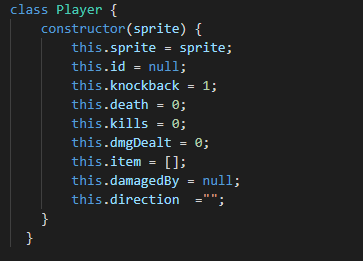
\includegraphics[scale=1]{pics/playerClass.PNG}
    \caption{Player-Klasse}
\end{figure}

Zum Erstellen der Player-Klasse wird zwar ein Sprite benötigt, damit der Player am Bildschirm angezeigt wird, aber es werden noch einige Attribute ergänzt:
\begin{compactitem}
    \item id: Zur eindeutigen Identifizierung
    \item knockback: Wert, der erhöht wird, desto öfter der Spieler getroffen wird; desto höher der Wert, desto weiter wird der Spieler von Projektilen weggestoßen
    \item death: Anzahl, wie oft der Spieler gestorben ist
    \item kills: Anzahl an Kills, die der Spieler gemacht hat (Abschüsse, die dazu geführt haben, dass der Gegner hinuntergefallen ist)
    \item dmgDealt: Anzahl, wie oft der Spieler jemanden getroffen hat
    \item item: Array von Items, die der Spieler gerade besitzt
    \item direction: String, der die Richtung angibt, in die der Spieler gerade schaut (links oder rechts)
\end{compactitem}

Während des Spiels werden auf der Map Items gespawned. Welcher Algorithmus dahinter steckt, wird im Kapitel \ref{impl:xCoordinates} genauer beschrieben.
Es wird zwischen 5 unterschiedlichen Items entschieden. Eine Item-Klasse hat ähnlich wie die Player-Klasse als Hauptbestandteil einen Sprite, doch auch hier werden noch weitere Attribute benötigt.

\begin{figure}[H]
    \centering
    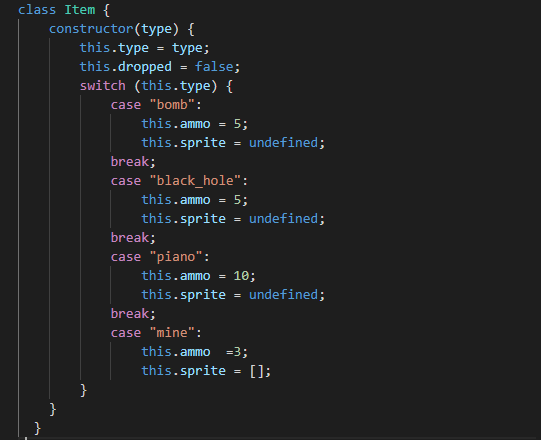
\includegraphics[scale=1]{pics/itemClass.PNG}
    \caption{Item-Klasse}
\end{figure}

\begin{compactitem}
    \item type: Gibt den Typ des Items an
    \item dropped: Gibt an, ob das Item irgendwo auf der Umgebung gelandet ist
    \item ammo: Anzahl, wie oft der Spieler das Item benutzen kann
\end{compactitem}

Je nachdem, welchen Typ das Item bekommen hat, wird auch die Anzahl wie oft
der Spieler es benutzen kann, verändert.
Wurde es zum Beispiel zum Type "bomb", kann der Spieler 5 Mal eine Bombe werfen.
\\
Bei dem Typ "mine", also einer Mine, kann der Spieler mehrere Minen gleichzeitig legen, deshalb ist das Sprite-Attribut auch ein Array.
Bei den anderen Items kann immer nur ein Sprite davon existieren.




\subsubsection{Die Items}  \label{impl:items}
Grundsätzlich gibt es 5 unterschiedliche Items in ScribbleFight. Je nachdem, welches Item der Spieler aufgesammelt hat, kann er oder sie verschiedene Fähigkeiten aktivieren.
Für jedes Item existiert eine Physik-Methode, die in der Draw-Funktion aufgerufen wird. Diese ist dafür verantwortlich, die physischen Eigenschaften der Items darzustellen. (zum Beispiel Gravitation)

\textbf{Keyboard-Access}
\\
Die Items werden alle durch Tasten auf der Tastatur ausgelöst. Durch p5.js kann sehr leicht auf die Tastatur zugriffen werden.
Mit der p5.js Methode <keyWentDown(Key)> wird überprüft, ob eine Taste gerade gedrückt wurde. (Als Parameter wird der ASCII-Code der gewünschten Taste übergeben)

\begin{lstlisting}[caption=Keyboard-Access,language=Java,label=lst:impl:keyboard-access]
    // E
    if (keyWentDown(69)) {
        bombAttack();
    }
    // Q
    if (keyWentDown(81)) {
        blackHoleAttack();
    }
    // R
    if (keyWentDown(82)) {
        pianoTime();
    }
    // C
    if (keyWentDown(67)) {
        placeMine();
    }
    // F
    if (keyWentDown(70)) {
        makeMeSmall();
    }
\end{lstlisting}

\textbf{Bomb}
\\
\textit{Das Bomben-Item wird mit der Taste <E> aktiviert.}
\\
Durch p5.play.js kann die vertikale Geschwindigkeit eines Sprites mit <sprite.velocity.y> verändert werden. Dadurch kann eine Gravitation simuliert werden.
Außerdem können mit der Methode <sprite.bounce(otherSprite)> Sprites an anderen Sprites oder Gruppen von Sprites 'abspringen'. Dies wird benutzt, damit die Bombe an der Umgebung abprallt.
Danach wird mit <sprite.overlap(myPlayer.sprite)> überprüft, ob eine Bombe mit meinem Spieler-Sprite kollidiert.
Falls ja, wird die Bombe mit <sprite.remove()> entfernt und mein Spieler wird weggestoßen.
Falls nein, wird noch überprüft, ob sich die Bombe außerhalb des Bildschirms befindet, und falls dies zutrifft, wird auch in diesem Fall die Bombe entfernt.
\\

\begin{lstlisting}[caption=Bomb Item Physics,language=Java,label=lst:impl:bombGravity]
    // verringern der vertikalen Geschwindigkeit 
    bomb.velocity.y -= GRAVITY;
    // bombe prallt an der Umgebung ab
    bomb.bounce(environment);

    // kollidert die Bombe mit meinem Player
    if(bomb.overlapSprite(myPlayer.sprite)) {
        // my Player gets knocked back
        myPlayer.sprite.getsThrownAway();
        // bomb gets deleted
        bomb.remove();
    } else if(bombIsOutsideMonitor()) {
        // bomb gets deleted
        bomb.remove();
    }

\end{lstlisting}

\textbf{Black Hole}
\\
\textit{Das Black-Hole-Item wird mit der Taste <Q> aktiviert}.
\\
Wie bei dem Bomben-Item wird auch bei dem Black-Hole-Item Gravitation simuliert. Jedoch nur für eine kurze Zeit, bis das Item in der Luft stehen bleibt und in einem Radius alle Spieler, die sich in diesem Radius befinden, anzieht, und diese auch alle Fähigkeiten nimmt.
Um zu überprüfen, wie lange das Item schon existiert, stellt p5.play.js das <life>-Attribut zur Verfügung. Dieser Wert ist ein Countdown, der sich bei jedem Draw-Zyklus um 1 verringert, bis sich das Item dann bei dem Wert 0 selbst löscht.
Damit das Item funktionieren kann, muss es andere Sprites anziehen können. Dazu wurde die attraction-Funktion von p5.play.js (mit leichten Veränderungen) benutzt:

\begin{lstlisting}[caption=Attraction,language=Java,label=lst:impl:attraction]
    // attraction
    if (myPlayer.sprite.overlap(b)) {
        noGravity = true;
        var angle = atan2(myPlayer.sprite.position.y - b.position.y, myPlayer.sprite.position.x - b.position.x);
        if (myPlayer.sprite.velocity.y >= -pixelWidth && myPlayer.sprite.velocity.y <= pixelWidth) {
          myPlayer.sprite.velocity.x -= cos(angle);
        }
        myPlayer.sprite.velocity.y -= sin(angle);
      }

\end{lstlisting}

Die Black-Hole-Physics Funktion sieht also (vereinfacht) so aus:
\\
\begin{lstlisting}[caption=Black Hole Item Physics,language=Java,label=lst:impl:bombGravity]
    // if the item has reached a certain life, make it static and attract players
    if (b.life <= 400) {
        attraction(b);
        b.velocity.y = 0;
        b.velocity.x = 0;
      }

      // if the item has not reached a certain life, let it bounce off the environment
      if (b.life > 400) {
        b.velocity.y -= GRAVITY;
        b.bounce(environment);
      }

      // if the item is outside of the monitor, delete it
      if (b.position.x > windowWidth || b.position.y > windowHeight || b.life == 0) {
        b.remove();
      }

\end{lstlisting}

\textbf{Piano}
\\
\textit{Das Piano-Item wird mit der Taste <R> aktiviert.}
\\
Das Piano-Item ist, wie der Namen schon vermuten lässt, ein Klavier, das am höchsten Punkt der Map erscheint und nach unten fällt.
Das bedeutet, die y-Koordinate ist 0 und die x-Koordinate ist die selbe wie die, die der Sprite des Spielers hat, der das Piano aktiviert hat.
Bei Kontakt zu einem Spieler oder der Umgebung wird das Klavier zerstört. Zum Überprüfen auf Kollisionen wird die p5.js Methode <sprite.collide(otherSprite)> verwendet.
Diese erhält den Wert \texttt{true}, falls eine Kollisionen zwischen zwei Sprites oder Sprite-Gruppen stattfindet.
\\
\begin{lstlisting}[caption=Piano-Item Physics,language=Java,label=lst:impl:pianoPhy]
    // check for collisions
    if (p.collide(environment)) {
        p.remove();
      } else if (p.overlap(myPlayer.sprite)) {
        myPlayer.sprite.getsThrownAway()
        p.remove();
      }
      p.velocity.y -= GRAVITY;
\end{lstlisting}

\textbf{Mine}
\\
\textit{Das Minen-Item wird mit der Taste <C> aktiviert.}
Das Minen-Item ist das einzige Item, bei dem der Spieler mehrere Instanzen auf einmal entsenden kann.
Es taucht hinter dem eigenen Player-Sprite auf und fliegt so lange nach unten, bis es auf der Umgebung landet. Erst wenn es wo gelandet ist, wird es 'aktiv'.
Wenn eine Mine aktiviert worden ist, und ein Spieler in Berührung mit dem Item kommt, wird dieser in die Luft gestoßen und die Mine wird gelöscht.
\\
\begin{lstlisting}[caption=Mine-Item Physics,language=Java,label=lst:impl:minePhy]
    // check if mine has landed somewhere (if true: activate mine)
    if (m.collide(environment) && m.touching.bottom) {
        m.set = true;
    }
    if (m.overlap(myPlayer.sprite) && m.set) {
        myPlayer.sprite.getsThrownAway();
        m.remove();
    }
    m.velocity.y -= GRAVITY;
\end{lstlisting}

\textbf{Size-Reduction}
\\
\textit{Das Size-Reduction-Item wird mit der Taste <F> aktiviert.}
\\
Dieses Item ist das einzige, das keinen eigenen Sprite hat. Das einzige was diese Item macht, ist, den Spieler-Sprite zu verkleinern. Dadurch wird dieser schwieriger zu treffen.
Wenn das Item aktiviert wird, wird der Sprite des Spielers verkleinert und ein Counter wird gestartet. Dieser wird alle 60 Frames um eins verringert. Ist der Counter 0, wird der Sprite wieder in seine Originalgröße gebracht.
Der Code, der dies umsetzt, sieht vereinfacht so aus:
\\
\begin{lstlisting}[caption=Size-Reduction,language=Java,label=lst:impl:sizeReduc]
// gets called on key press F
function makeMeSmall() {
  if (doIHaveTheItem()) {
    imSmall = true;
    smallTimer = 10;
  }
}

// gets called in draw function
function smallChecker() {
  if (imSmall) {
    // scale the sprite down at the start of countdown
    if (smallTimer == 10) {
      myPlayer.sprite.scale = 0.6;
    }
    // every second (60 frames), the countdown gets reduced
    if (frameCount % 60 == 0 && smallTimer > 0) {
      smallTimer--;
    }
    // if the countdown is over, rescale the sprite back to the original form
    if (smallTimer == 0) {
      myPlayer.sprite.scale = 1;
      smallTimer = 10;
      imSmall = false;
    }
  }

}
\end{lstlisting}

\textbf{Die Default-Attacke}
\\
\textit{Die Default-Attacke wird mit <Left-Click> aktiviert.}
\\
p5.js bietet sehr leicht die Möglichkeit, auf User-Input zu überprüfen. Das einzige, was nötig ist um zu erkennen, ob der User gerade die linke Maustaste geklickt hat, ist die Funktion <mouseClicked()>.
Mit dieser Funktion wird nun zu dem Punkt, auf dem der Spieler gerade die Maus hält und die Default-Attacke aktiviert, ein Projektil abgeschossen. Um die Information zu erhalten, auf welcher X- und Y-Position sich die Maus befindet,
werden die von p5.js vordefinierten Eigenschaft <camera.mouseX> und <camera.mouseY> verwendet.
\\
\begin{lstlisting}[caption=Default-Attacke,language=Java,label=lst:impl:defaultAttack]
    function mouseClicked() {
    // Maus-Position
    let x = camera.mouseX,
        y = camera.mouseY;
    // Sprite wird bei meiner Player-Sprite-Positon erstellt
    projectile = createSprite(myPlayer.sprite.position.x, myPlayer.sprite.position.y, pixelWidth, pixelWidth);
      
    // Geschwindigkeit wird auf die Position der Maus ausgerichtet
    projectile.velocity.x = (x - myPlayer.sprite.position.x);
    projectile.velocity.y = (y - myPlayer.sprite.position.y);
}

\end{lstlisting}

\subsubsection{Movements}
Es gibt 3 fundamentale Bewegungsmöglichkeiten in ScribbleFight. Springen, links/rechts laufen und 'klettern'. Diese Bewegungen werden im Folgenden genauer erläutert.

\textbf{Springen}
\\
In dem Web-Game kann der Spieler mittels Leertaste springen. Genau wie bei den Item-Aktivierungen, wird mithilfe von p5.js Methoden der User-Input ermittelt.
Bei dem Springbewegung wird einfach die vertikale Geschwindigkeit des Spieler-Sprites so verändert, dass dieser etwas nach oben springt.
\\
\begin{lstlisting}[caption=Jumping,language=Java,label=lst:impl:jumping]
    // check if user pressed spacebar
    if (keyWentDown(32)) {
        jump()
    }

    function jump() {
    // user is only allowed to jump 2 times (it resets when touching the ground)
    if (!(JUMP_COUNT >= MAX_JUMP)) {
        // make the user fly up a bit (JUMP is a global variable)
        myPlayer.sprite.velocity.y = -JUMP;
        JUMP_COUNT++;
    }
}
\end{lstlisting}

\textbf{Links/Rechts Laufen}
\\
Das Prinzip des Links oder Rechts Bewegens ist sehr simpel. Es wird einfach die horizontale Geschwindigkeit des Player-Sprites auf eine konstante Variable gesetzt.
Wenn sich der Spieler nach rechts bewegt, ist diese Konstante positiv, bei einer Linksbewegung negativ. Im Gegensatz zur Springbewegung wird diesmal aber die Methode <keyIsDown(key)> verwendet, und nicht <keyWentDown(key)>.
Der Grund dafür ist, dass die Bewegung so lange anhalten soll, wie der User die Taste drückt, und nicht nur einmal pro Tastendruck.

\begin{lstlisting}[caption=Links/Rechts-Movement,language=Java,label=lst:impl:moving]
    //A
    if (keyIsDown(65)) {
        moveLeft()
    }
    //D
    if (keyIsDown(68)) {
        moveRight()
    }

    // SPEED is a global variable
    function moveLeft() {
    myPlayer.sprite.velocity.x = -SPEED;
    }

    function moveRight() {
    myPlayer.sprite.velocity.x = SPEED;
    }
\end{lstlisting}

\textbf{Bewegung auf der Spielumgebung}
\\
Die Bewegung auf der Spielumgebung wird durch die Methode <collisions()> bestimmt. Diese wird in der draw-Methode aufgerufen und wird somit 60 mal die Sekunde ausgeführt.
Berührt der Sprite des Players nichts, fällt er er mit konstanter Geschwindigkeit nach unten.
Findet jedoch eine Kollision mit der Spielumgebung statt, dann wird überprüft, welche Art von Berührung gerade stattfindet:

\begin{compactitem}
    \item Falls Berührung seitlich stattfindet: Player-Sprite bekommt eine Klettergeschwindigkeit und behält diese so lange, wie die Berührung stattfindet
    \item Falls Berührung unten stattfindet: Die vertikale Geschwindigkeit des Player-Sprites wird auf 0 gesetzt und der Sprung-Counter zurückgesetzt
    \item Falls Berührung oben stattfindet: Mit einer Berührung die zwischen Spielumgebung und Sprite stattfindet, kann der Spieler oder die Spielerin weder 'klettern' noch wird der Sprung-Counter zurückgesetzt
\end{compactitem}

\begin{lstlisting}[caption=Bewegung auf der Spielumgebung,language=Java,label=lst:impl:collisions]
    // check for collisions
    if (myPlayer.sprite.collide(environment)) {
      // if the collision is on the side, the sprite will start "climbing" with a certain speed
      if (myPlayer.sprite.touching.left || myPlayer.sprite.touching.right) {
        myPlayer.sprite.velocity.y = CLIMBINGSPEED;
      }
      // standing on the environment
      if(myPlayer.sprite.touching.bottom) {
        myPlayer.sprite.velocity.y = 0; 
      }
      // jump count gets only reset when the collision is not on the top of the player-sprite
      if (!myPlayer.sprite.touching.top) {
        JUMP_COUNT = 0;
      }
    }
\end{lstlisting}

\textbf{Knockback-Bewegung} \\
Wenn der Spieler von einem Projektil getroffen wurde, wird der eigene Player-Sprite für kurze Zeit bewegungsunfähig und prallt von der Spielumgebung ab.
Wie lang dieses Knockback-Movement andauert, kommt auf die Art des Projektils und auf den Wert des Knockbacks des Players an.
Soll der Player-Sprite also nun diese Bewegung ausführen, wird das mit einer Funktion namens <sendHimFlying()> bewerkstelligt.
Bevor diese aufgerufen wird, muss noch der Countdown, wie lange der Sprite nun in dieser Bewegung bleiben soll, festgelegt werden. Bei jedem draw-Zyklus wird dieser Countdown um den Wert eins verringert.
Hinzu kommt, dass wenn der Spieler getroffen wurde, er kurz etwas verlangsamt wird. Es soll so wirken, als wäre er gerade etwas betäubt worden.
\begin{lstlisting}[caption=Knockback-Bewegung,language=Java,label=lst:impl:knockbackMov]
// before function gets called, make sure to set flying to true and set a flying-duration
function sendHimFlying() {
  if (flying) {
    timeFlying--;
    //slowdown but only at the first half of flying-duration
    if (timeFlying <= flyingDuration / 2 && timeFlying > 0) {
      if (myPlayer.sprite.velocity.x > 0) { myPlayer.sprite.velocity.x -= 0.3; }
      if (myPlayer.sprite.velocity.x < 0) { myPlayer.sprite.velocity.x += 0.3; }
      if (myPlayer.sprite.velocity.y > 0) { myPlayer.sprite.velocity.y -= 0.3; }
      if (myPlayer.sprite.velocity.y < 0) { myPlayer.sprite.velocity.y += 0.3; }
    }
    // flying-duration is over
    if (timeFlying == 0) {
      flying = false;
    }
  }
}
\end{lstlisting}


\textbf{Richtungswechsel des Sprites} \label{directionChange}
\\
Ein weiterer wichtiger Aspekt bei der Bewegung des Player-Sprites ist, dass sich auch die Orientierung des Bildes ändern muss, wenn dieser die Richtung wechselt.
Auch für diese Problemstellung stellt p5.play.js eine Lösung zu Verfügung. Mit der Methode <mirrorX()> wird der Sprite entlang seiner vertikalen Achse gespiegelt.
Jedes mal, wenn der User nun also die Richtung seines Player-Sprites wechselt, wird auch der Sprites passend seiner Bewegung gespiegelt.

\begin{lstlisting}[caption=Sprite Richtungswechsel,language=Java,label=lst:impl:mirrorSprite]
    function mirrorSprite() {
        // A
        if (keyWentDown(65)) {
            mirrorSpriteLeft()
        }
        // D
        if (keyWentDown(68)) {
            mirrorSpriteRight()
        }
    }
    
    function mirrorSpriteLeft() {
        // if the mirrorX attribute is 1, then the sprite is looking to the right
        if (myPlayer.sprite.mirrorX() === 1) {
            myPlayer.sprite.mirrorX(myPlayer.sprite.mirrorX() * -1);
            myPlayer.direction = "left";
        }
    }
    
    function mirrorSpriteRight() {
        // if the mirrorX attribute is 1, then the sprite is looking to the left
        if (myPlayer.sprite.mirrorX() === -1) {
            myPlayer.sprite.mirrorX(myPlayer.sprite.mirrorX() * -1);
            myPlayer.direction = "right";
        }
    }
\end{lstlisting}

\subsubsection{Wie gewinne ich?} \label{impl:win}
Um in ScribbleFight zu gewinnen, muss der Spieler oder die Spielerin seinen Gegner/seine Gegner drei mal erfolgreich von der Spielumgebung schießen, so, dass der Sprite des Gegners ins 'Nichts' fällt.
Dies ist durch die Attacken, die in Kapitel \ref{impl:items} genau beschreiben werden, möglich.
Um zu überprüfen, ob der Sprite nun hinuntergefallen und somit 'gestorben' ist, wird in der draw-Methode die Funktion <deathCheck()> aufgerufen.
Diese hat einige Aufgaben:
\begin{compactitem}
    \item Überprüfen ob sich der Player-Sprite außerhalb des Bildschirms befindet
    \item Falls ja, überprüfen ob der Player noch mindestens ein Leben hat
    \item Falls der Player keine Leben mehr hat, wird sein Sprite zerstört
    \item Hat der Player noch weitere Leben, dann wird er nach drei Sekunden an einem zufälligen Punkt, an dem er nicht direkt wieder aus dem Bildschirm fällt, gespawned
    \item Wird der Player respawned, werden ihm alle seine Items, die er eventuell noch hatte, wieder genommen
    \item Wird der Player respawned, wird sein Knockback wieder zurückgesetzt
\end{compactitem}

Vereinfacht sieht die Methode also so aus:

\begin{lstlisting}[caption=Überprüfung nach Toden,language=Java,label=lst:impl:deathCheck]
function deathCheck() {
    // check if sprite has fallen outside of the monitor
    if (myPlayer.sprite.position.y - player_height > windowHeight) {
        youDied();
    }
}

function youDied() {
    myPlayer.removeItem();
    myPlayer.death++;
    myPlayer.knockback = 1;

    // after 3 seconds the player gets respawned on a location, if he still has at least one live left
    setTimeout(() => {
        if (myPlayer.death < 3) {
            myPlayer.sprite.position.x = xCoordinates[Math.floor(Math.random() * xCoordinates.length)];
            myPlayer.sprite.position.y = 0;
        }
    }, 3000);
}
\end{lstlisting}

Außerdem zählt es auch als Tod, wenn der Knockback des eigenen Players über einen gewissen Wert ansteigt. Dies wird mit der <fatalHit()>-Methode überprüft.
Diese Methode wird immer dann aufgerufen, wenn der eigene Player von irgendeinem Projekil getroffen wurde.
\begin{lstlisting}[caption=Fatal Hit,language=Java,label=lst:impl:fatalHit]
    function fatalHit() {
        if (myPlayer.knockback > MAX_KNOCKBACK) {
            youDied();
        }
    } 
\end{lstlisting}
Ein Indikator, ob der Spieler gut abgeschnitten hat, sind die Kills, die er erzielen konnte.
In ScribbleFight kann der Spieler Kills sammeln, indem er jemanden mit jeglicher Art von Projektil trifft, und dieser innerhalb von 3 Sekunden aus der Spielumgebung fliegt.
Dies funktioniert so, dass wenn jemand meinen player-Sprite trifft, in meinem Player-Objekt abgespeichert wird, welcher Spieler mich gerade getroffen hat.
Diese Information wird aber alle 3 Sekunden wieder gelöscht.

\begin{lstlisting}[,language=Java]
    function draw() {
        // every second, the countdown gets reduced by 1
        if (frameCount % 60 == 0 && damagedByTimer > 0 && myPlayer.damagedBy != null) {
            damagedByTimer--;
          }
      
        // if the countdown has reached 0, the information gets deleted and the countdown restarts
        if (damagedByTimer == 0) {
            damagedByTimer = 3;
            myPlayer.damagedBy = null;
        }
    }
   
\end{lstlisting}


Wenn ich nun sterbe, und die Information, dass mich jemand getroffen hat in meinem Player-Objekt gespeichert ist, bekommt dieser einen Kill.



\subsubsection{Erstellung der Spielumgebung} \label{impl:Spielumgebung}
Um sich auch auf dem Bild, das der User gezeichnet hat, bewegen zu können, müssen einiges Schritte durchgeführt werden. Mittels Objekterkennung kann das Bild abfotografiert,
und daraus ein Array mit Bildaten erstellt werden, aus dem dann die Spielumgebung kreiert wird. Wie genau dieser Array zustande kommt, wird in Kapitel \ref{maai:udbifdsbd:head} beschrieben.
\\
\begin{lstlisting}[caption=Vereinfachte Darstellung eines Bilddaten-Arrays,language=Java,label=lst:impl:bilddaten]
    [[0, 0, 0, 0], [0, 0, 0, 0], [0, 0, 0, 0],
    [0, 0, 0, 0], [0, 0, 0, 0], [0, 0, 0, 0],
    [0, 0, 0, 0], [0, 0, 0, 0], [0, 0, 0, 0],
    [255, 255, 255, 0], [252, 252, 252, 0], [251, 251, 251, 0],
    [248, 248, 248, 0], [249, 249, 249, 0], [247, 247, 247, 0],
    [255, 255, 255, 0], [240, 240, 240, 0], [250, 250, 250, 0],
    [174, 174, 174, 0], [255, 255, 255, 0], [173, 173, 173, 0],
    [226, 226, 226, 0], [255, 255, 255, 0], [253, 253, 253, 0],
    [163, 163, 163, 0], [254, 254, 254, 0], [255, 255, 255, 0],
    [0, 0, 0, 0], [0, 0, 0, 0], [[0, 0, 0, 0],
\end{lstlisting}


Desto genauer dieser Array ist, desto genauer werden auch die Hitboxen der Spielumgebung, denn die gezeichneten Formen werden mit Rechteck-Hitboxen nachgestellt.
Eine Hitbox ist ein Bereich, der für die Berechnung für Kollision benutzt wird.
Hat ein Eintrag des Arrays an Stelle vier mehr als 0 als Wert, wird dort ein Pixel erstellt. Das liegt daran, dass an der vierten Stelle eines solchen Eintrags die Deckkraft der Bildstelle angegeben wird. Das bedeutet, der User hat dort etwas gezeichnet.
Natürlich muss der Sprite-Pixel noch einen richtigen X- und Y-Wert bekommen. Diese Koordinate muss auch mit dem Punkt des Bildes übereinstimmen, an den der Sprite als Hitbox agieren soll.
Aus Perfomance-Gründen (Es wird durchgehend auf Kollidierung zwischen Player und Spielumgebung geprüft) werden die Sprite-Pixel entlang der X-Achse noch zusammengefasst.
Wurden nun alle Sprite-Pixel ausfindig gemacht, mit richtigen Koordinaten versehen und entlang der horizontalen Achse zusammengefasst, werden alle einer p5-Group-Variable hinzugefügt.
Das macht das Überprüfen auf Kollision sehr leicht. \\
Die nächsten drei Bilder sollen den Ablauf bildlich darstellen.

Zuerst das originale, vom User gezeichnete Bild.
\begin{figure}[H]
    \centering
    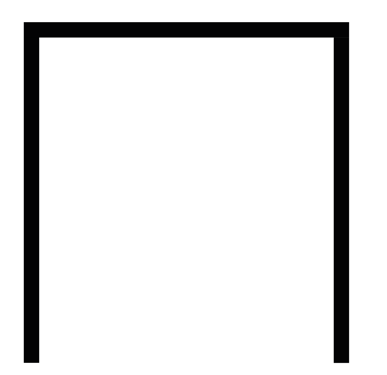
\includegraphics[scale=0.5]{pics/simpleDrawing.PNG}
    \caption{Originale Zeichnung}
\end{figure}

Aus diesem Bild kann ein Array aus Bilddaten erstellt werden. Wenn aber einfach mit diesem Array
die Pixel für die Spielumgebung erstellt, sind diese noch viel zu klein und an der falschen Position.
\\
\begin{figure}[H]
    \centering
    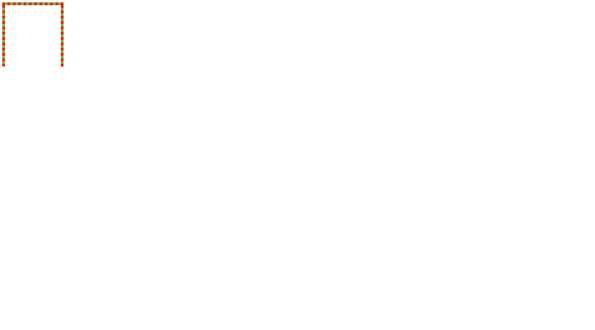
\includegraphics[scale=0.5]{pics/simpleDrawing2.PNG}
    \caption{Bilddaten-Array bildich dargestellt}
\end{figure}

Um die richtigen Koordinaten für die Sprite-Pixel zu bestimmen, werden noch einige andere Faktoren miteinbezogen und daraus dann die richtige Position der Pixel am Bildschirm ermittelt.
Außerdem werden sie noch entlang der X-Achse kombiniert.

\begin{figure}[H]
    \centering
    
\includegraphics[scale=0.75]{pics/simpleDrawing3.PNG}
    \caption{Spielumgebung}
\end{figure}

Natürlich werden dann diese Sprites versteckt. Es soll ja so wirken, also würde sich der User auf dem, was er gerade gezeichnet hat, bewegen können.
Im Folgenden wird der Algorithmus zum Aufbereiten der Spielumgebung vereinfacht dargestellt.
\begin{lstlisting}[,language=Java,label=lst:impl:createEnv]
    environment = new Group();
    // looping through image data array
    for (let i = 0; i < pixel_clumps.length; i++) {
      sprite_pixels[i] = [];
      for (let j = 0; j < pixel_clumps[0].length; j++) {
        if the value is greater than 0, then something has been drawn there
        if (pixel_clumps[i][j][3] > 0) {
          //if the last value in the array is not undefined, we can merge the sprite-pixels
          if (sprite_pixels[i][j - 1] !== undefined) {
            same_x_counter++;
            sprite_pixels[i][j] = createSprite(pixelWidth * faktorX, pielWidth * faktorY, pixelWidth * same_x_counter, pixelWidth);
            // add sprite to environment group
            environment.add(sprite_pixels[i][j]);
            // remove the last value, because it has been replaced by a new sprite, with a greater width
            sprite_pixels[i][j - 1].remove();
            sprite_pixels[i][j - 1] = undefined;
          } else {
            same_x_counter = 1;
            sprite_pixels[i][j] = createSprite(pixelWidth * faktorX, pielWidth * faktorY, pixelWidth, pixelWidth); 
            // add sprite to environment group
            environment.add(sprite_pixels[i][j]);
          }
        }
      }
    }
\end{lstlisting}

\subsubsection{Item-Spawns} \label{impl:itemSpawnF}
Alle 10 Sekunden wird ein Item erstellt.
Es wird an oberster Stelle des Bildschirms kreiert (y-Koordiante = 0); die x-Position dieses Items wird dann zufällig ausgewählt.
Wichtig dabei ist jedoch, dass das Items auf keiner Position spawnen darf, bei der es einfach oben auftaucht und dann aus dem Bildschirm fällt.
Wie diese x-Koordiaten berechnet werden, wird in Kapitel \ref{impl:xCoordinates} genau beschrieben.
Damit die Items voneinander unterschieden werden können, wird jede Art von Item farblich gekennzeichnet:

\begin{compactitem}
    \item Rot: Bomb
    \item Blau: Black-Hole
    \item Gelb: Piano
    \item Orange: Mine
    \item Grün: Size-Reduction
\end{compactitem}

Den Input, wann ein Item genau erstellt wird, (muss bei jedem User der gerade spielt gleich sein) liefert der Server. Genauere Details wie der Server von des Web-Games funktioniert, wird in Kapitel \ref{impl:itemSpawnB} beschrieben.
\\

\begin{lstlisting}[caption=Erstellen eines Items,language=Java,label=lst:impl:createItem]
funciton createItem(data) {
    // number between 1-5 from the server to create a random item
    let num = data.num;
    // random x-Coordinate from the server
    let x = data.x
    // this equation gets you the highest point of the map
    let y = (windowHeight - ImageHeight) / 2;
    // if x = -1, something on the server-side went wrong
    if (x != -1) {
        // itemSize is a global variable
        switch (num) {
            case 1:
                i = createSprite(x, y, itemSize, itemSize);
                i.type = "bomb";
                break;
            case 2:
                i = createSprite(x, y, itemSize, itemSize);
                i.type = "black_hole";
                break;
            case 3:
                i = createSprite(x, y, itemSize, itemSize);
                i.type = "piano";
                break;
            case 4:
                i = createSprite(x, y, itemSize, itemSize);
                i.type = "mine";
                break;
            case 5:
                i = createSprite(x, y, itemSize, itemSize);
                i.type = "small";
                break;
        }
        i.dropped = false;
        items.push(i);
    }
\end{lstlisting}

Nachdem nun das Item erstellt wurde, braucht dieses natürlich auch so wie zum Beispiel die Projektile oder der Player eine eigene Physik-Methode. Diese wird, so wie die anderen Physik-Methoden auch, in der Draw-Methode aufgerufen.
Die Methode funktioniert so, dass das Item so lange fällt, bis es irgenwo auf der Spielumgebung landet. Jeder Player kann jeder Zeit das Item berühren und somit eine neue Fähigkeit bekommen.

\begin{lstlisting}[caption=Item-Physik,language=Java,label=lst:impl:itemPhy]
    function itemPickUp() {
        if (items.length > 0) {
            items.forEach(item => {
                // if the item collides with the environment, the dropped-attribute becomes true
                if(item.collide(environment)) {
                    item.dropped = true;
                }
                // if the item has not landed anywhere, let it fall 
                if(!item.dropped) {
                    item.velocity.y -= GRAVITY;
                }
    
                // if I collide with the item, I get a new ability depending on the type of the item and the item gets deleted
                if (item.overlap(myPlayer.sprite)) {
                    myPlayer.item[item.type] = new Item(item.type);
                    deleteItem(item);
                }
        }
    }
    \end{lstlisting}

\textbf{Bestimmung von gültigen X-Koordinaten} \label{impl:xCoordinates}
\\
Mit gültiger X-Koordinaten sind jene X-Koordinaten gemeint, bei denen ein Sprite erstellt werden kann, und dieser dann irgendwo auf der Spielumgebung landet und nicht sofort aus dem Bildschirm fliegt.
Bei dem Algorithmus wird zuerst überprüft, auf welchen Stellen Sprite-Pixel (Pixel aus denen die Spielumgebung besteht) vorhanden sind. Von diesen kann schon der Mittelpunkt als gültige X-Koordiaten genommen werden, solange dieser Pixel eine gewisse Breite aufweist.
Doch damit bei einem sehr breiten Pixel nicht nur eine einzige X-Koordinate ausgewählt wird, wird schrittweise überprüft, ob noch Stellen vor oder hinter dem Mittelpunkt des Sprites in Frage kommen.
Dazu wird dieser Sprite-Pixel nach vorne und nach hinten abgetastet, ob noch genügend Platz da ist, ein Item dort landen zu lassen.
Es können höchstens halb so viele X-Koordiaten pro Sprite-Pixel ausgewählt werden, wie der Pixel (in Pixel-Width gemessen) breit ist.
Die Funktion wird im Setup von ScribbleFight aufgerufen.

\begin{lstlisting}[caption=Bestimmung gültiger X-Koordinaten,language=Java,label=lst:impl:xCoords]
    function getXCoordinates() {
        let sprite;
        // looping through the sprite_pixel array
        for (let i = 0; i < sprite_pixels.length; i++) {
            for (let j = 0; j < sprite_pixels[i].length; j++) {
                sprite = sprite_pixels[i][j];
                // if the sprite variable is not undefined, it means a sprite exists there
                // the sprite hast to be a width of at least 4 times the normal pixel width
                if (sprite !== undefined && sprite.width >= pixelWidth * 4) {
                    // sprites gets checked if there are more Coordinates to let an item spawn there (to the right of the center)
                    for (let index = 0; index < sprite.width / 2; index += pixelWidth * 2) {
                        if (sprite.position.x + index < sprite.position.x + sprite.width / 2) {
                            let x = sprite.position.x + index;
                            xCoordinates.push(x);
                        }
                    }
                    // sprites gets checked if there are more Coordinates to let an item spawn there (to the left of the center)
                    for (let index = sprite.width; index > sprite.width / 2; index -= pixelWidth * 2) {
                        if (sprite.position.x + index > sprite.position.x + sprite.width / 2) {
                            let x = sprite.position.x + index - sprite.width;
                            xCoordinates.push(x);
                        }
                    }
                    // doing this eliminates duplicates
                    xCoordinates = Array.from(new Set(xCoordinates));
                }
            }
            return xCoordinates;
        }
    }
\end{lstlisting}

\textbf{Progressbar} \label{impl:progressbar} \\
Um dem Spieler Feedback zu geben, wie oft er getroffen wurde, wird eine Progressbar am oberen Rand des Bildschirms eingefügt. Je öfter man getroffen wurde, desto mehr füllt sich diese.
Wenn die Progressbar komplett aufgefüllt ist, wird der nächste Treffer eines Projektils den Spieler umbringen.
Umgesetzt wurde dieses Feature, indem man den derzeitigen Knockback des Spieler auf den Bereich zwischen 0 bis zur Hintergrundsbild-Breite mapped. Dazu wurde die von p5.js vordefinierte Funktion \texttt{map} verwendet.
Als Parameter nimmt diese Funktion:
\begin{compactitem}
    \item Der umzuwandelnde Wert
    \item Start-Wert des ersten Bereichs
    \item End-Wert des ersten Bereichs
    \item Start-Wert des zweiten Bereichs
    \item End-Wert des zweiten Bereichs
\end{compactitem}
\begin{lstlisting}[language=Java, caption=Progressbar,label=lst:impl:progressbar]
//gets called in setup function
function createUI() {
    // position the progressbar at the top of the background-image
    // at the start, the width is of the progessbar is 0
    progressBar = createSprite(windowWidth/2 ,(windowHeight-ImageHeight) / 2,0, width);
    progressBar.position.x += progressBar.width / 2;
    progressBar.position.y += progressBar.height / 2;
    progressBar.shapeColor = color(255,0,0);
}
// gets called whenever my player is hit
function updateUI() {
  let progress;
  progress = map(myPlayer.knockback,1,MAX_KNOCKBACK,0,newImageWidth);
  progressBar.width = progress;
}
\end{lstlisting}

\subsection{Server [R]}
Der Server von des Spiels ist ein einfacher Web-Server, der mit Node.js und express.js umgesetzt wurde.
Dieser hostet statische Files, auf denen sich der Code für das Frontend befindet (HTML Files, p5.js library, etc).
Viele Teile dieses Codes werden im vorherigen Kapitel detailliert erklärt.
Durch SocketIO können multiple Clients eine Verbindung mit dem Server aufbauen.
So wird es ermöglicht, dass unterschiedliche Clients gemeinsam spielen können.

\subsubsection{Erstellen des Servers}
Ein Node.js Server ist einfach zu erstellen. Zwei Voraussetzungen müssen vorhanden sein:

\begin{compactitem}
    \item Eine funktionierende Node.js-Version
    \item JavaScript Grundlagen
\end{compactitem}

Ist dies gegeben, kann ein neuen Ordner erstellt, und in diesem dann der Befehl \texttt{npm init} ausgeführt werden.
Dort wird dann ein package.json File für das Node-Projekt erstellt. Nähere Infos zu diesem File kann in Kapitel \ref{NPM} nachgelesen werden.
Danach kann entweder durch eine Entwicklungsumgebung ein neues JavaScript File erstellt, oder im Terminal der Befehl \texttt{touch server.js} eingegeben werden.
In dem Backend von ScribbleFight werden express.js und SocketIO benutzt, deshalb müssen die Befehle \texttt{npm install express --save} für express.js, und
\texttt{npm install socket.io} für SocketIO im Terminal ausgeführt werden. Dies installiert die Module und fügt die Dependencies zu dem package.json-File hinzu.

Wurde all das berücksichtigt, wird jetzt die Logik des server.js-Files umgesetzt. Zuerst wird eine Instanz von express.js erstellt.
Danach wird ein HTTP-Server-Objekt und eine SocketIO Instanz angelegt, die das HTTP-Server-Objekt als Paramter nimmt. Zusätzlich wird noch Cross-Origin Resource Sharing freigegeben.
Der Code sieht also so aus:

\begin{lstlisting}[caption=,language=Java,label=lst:impl:socketIO]
    var express = require("express");
    var app = express();
    var http = require("http").createServer(app);
    var io = require("socket.io")(http, {
        cors: {
            origin: '*',
        }
    });
\end{lstlisting}

Das war aber nur ein Teil, um einen funktionierenden SocketIO-Webserver zu erstellen. Bei unserem Web-Game müssen, wie vorher schon erwähnt, das Frontend als statische Files gehostet werden.
Für dieses Problem wurde das Paths-Module von Node.js verwendet. Dieses stellt Funktionen für das Arbeiten mit File-und Directory-Pfaden zur Verfügung. Darauf zugegriffen werden wird mit:

\begin{lstlisting}[caption=,language=Java,label=lst:impl:socketIO]
    const path = require('path');
\end{lstlisting}

Nun können die Files einfach mit \\

\begin{lstlisting}[caption=,language=Java,label=lst:impl:socketIO]
    // path.join is used to get the right path 
    app.use(express.static(path.join(__dirname, '/../p5_frontend/src')));
\end{lstlisting}

gehostet werden. (Diese befinden sich in dem Folder <src>);

Als letzten Schritt wird noch der Port bei dem HTTP-Server-Objekt angegeben, im Fall von unserem Server ist dieser 3000.
\begin{lstlisting}[caption=,language=Java,label=lst:impl:socketIO]
    // Server is listening on port 3000
    http.listen(3000);
\end{lstlisting}

Ist das alles abgeschlossen, wird nun die SocketIO Logik umgesetzt.

\subsubsection{SocketIO Logik}
Der nun funktionierende Web-Server soll nun SocketIO-Verbindungen, die vom Browser kommen, annehmen können.
Mit der SocketIO Instanz, die im letzten Abschnitt erstellt worden ist, kann dieses Problem sehr leicht gelöst werden:

\begin{lstlisting}[caption=,language=Java,label=lst:impl:socketIO]
    io.sockets.on('connection', newConnection);

    function newConnection(socket) {
        // LOGIC COMES HERE
    }
\end{lstlisting}

Findet nun eine Verbindung zu dem Server von einem Client statt, wird die Methode <newConnection(socket)> aufgerufen.
Der Parameter der Methode ist eine Socket-Instanz, die sehr viele Informationen und Funktionalitäten der gerade bestehenden Verbindung enthält.
Wie der Client eine Verbindung zu diesem Server aufbauen kann, ist von Programmiersprache zu Programmiersprache unterschiedlich. Im Frontend von ScribbleFight wird JavaScritp benutzt.

\textbf{SocketIO im Frontend}

Um im Frontend eine SocketIO-Verbindung aufzubauen, wird zuerst in dem index.html File die SocketIO Library verlinkt:
\begin{lstlisting}[,language=Java,label=lst:impl:socketIO]
    // link SocketIO in index.html
    <script src="https://cdn.socket.io/4.1.2/socket.io.min.js"></script>
\end{lstlisting}

Jetzt kann einfach eine neue Socket-Instanz erstellt werden mit der der Client Events empfangen, aber auch aussenden kann.
Da der Server von ScribbleFight nicht mehr lokal läuft, sondern auf einem Kubernetes-Cluster, wird hierbei noch ein Pfad definiert, um eine korrekte Instanz zu erstellen.

\begin{lstlisting}[,language=Java,label=lst:impl:socketIO]
    var socket = io({
        path: "/t.rafetseder/scribble-fight/socket.io"
      }); 
\end{lstlisting}

Einfach nur der Befehl \texttt{io()} würde die Pfad-Parameter (/t.rafetseder/scribble-fight/socket.io) der derzeiten Domaine einfach ignorieren und die Verbindung könnte nicht hergestellt werden.
\\
Nun können mit dem Befehl
\texttt{socket.on('event',funciton)} Events empfangen, und mit \texttt{socket.emit('event')} Events ausgelöst werden.

\textbf{SocketIO Events} \\
Nachdem nun eine aufrechte Verbindunge hergestellt werden konnte, gibt es 10 Events, die passieren können.
\begin{compactitem}
    \item Ein neuer Spieler soll erstellt werden
    \item Abruf von schon bestehenden Spielern
    \item Die Position von meinem Sprite soll aktualisiert werden
    \item Die Richtung, in die mein Sprite schaut, soll aktualisiert werden
    \item Ein Item wurde aufgehoben, also soll es bei jedem entfernt werden
    \item Jemand hat eine Attacke ausgeführt, also soll bei jedem ein Projektil erstellt werden
    \item Jemand hat einen Kill erzielt
    \item Ein Spieler wurde von einem Projektil getroffen, das heißt das Projektil, das getroffen hat, muss bei jedem entfernt werden
    \item Jemand ist gestorben
    \item Es soll ein neues Item erstellt werden (Passiert alle 10 Sekunden)
\end{compactitem}

Diese Events werden im Folgenden genau erklärt.

\textbf{Erstellen eines neuen Spielers und Abrufen von vorhandenen Spieler} \\
Führt der Spieler das Frontend aus, stellt dieses sofort eine Verbindung mit dem Sever her. Um nun schon vorhandene Spieler, die gerade auch verbunden sind zu erhalten, wird ein Event <getPlayers> emittiert.
Danach muss dem Server noch mitgeteilt werden, dass der Spieler nun selbst auch eine spielbare Figur erhlaten möchte. Dies wird mit dem <newPlayer>-Event bewerkstelligt.
Wird nun das Event <newPlayer> vom Server ausgelöst, wird ein neues Player-Objekt dem Player-Array des Frontends hinzugefügt. Der Konstruktur von diesem Player-Objekt benötigt nur einen Sprite, der auch neu erstellt wird.
\begin{lstlisting}[,language=Java,label=lst:impl:socketIO]
    // listen to an event from the server
    socket.on('newPlayer',createNewPlayer);
    // get existing players
    socket.emit('getPlayers');
    // create my own player
    socket.emit('newPlayer');

    function createNewPlayer(data) {
        // new player gets added an new sprite is created in the middle of the map
        players[data.id] = new Player(createSprite(ImageWidth / 2,ImageHeight / 2, player_width, player_height));
    }
\end{lstlisting}

Im Server sieht das Ganze etwas komplizierter aus. Grundsätzlich speichert der Server alle Player-Objekte in einem Map-Objekt ab.
Die ID für jedes dieser Player-Objekte dient einfach die ID der Socket-Verbindung. Will ein Client nun alle schon vorhandenen Spieler, wird die Map (falls Spieler vorhanden) durchlaufen, und die ID von jedem der Spieler an den anfragenden Client geschickt.
Dieser erstellt dann einen neuen Player / mehrere neue Player mit der dazugehörigen ID.

\begin{lstlisting}[,language=Java,label=lst:impl:socketIO]
    socket.on('getPlayers',sendPlayers);

    // the object players is the map that has the player-objects saved
    function sendPlayers() {
        if (players.size > 0) {
            players.forEach((values, keys) => {
                let data = {
                    id: values.id,
                }
                socket.emit('newPlayer', data);
            })
        }
    }
\end{lstlisting}

Nachdem nun der Server alle schon vorhanden Spieler dem Client mitgeteilt hat, muss noch ein neuer Spieler für diesen Client erstellt werden.

\begin{lstlisting}[,language=Java,label=lst:impl:socketIO]
    socket.on('newPlayer',createPlayer);  

    function createPlayer() {
        players.set(socket.id, new Player(socket.id));
        let data = {
            id: socket.id,
        }
        // im using io.emit() so it sends to everyone, including the client that triggered the event
        io.emit('newPlayer', data);
    }
\end{lstlisting}

Der Client erstellt nun genau gleich wie bei dem <getPlayers>-Event den Spieler.

\textbf{Update Position and Update Direction}

Die Postion des Sprites von jedem Spieler soll in jedem Draw-Zyklus geupdatet werden. Die Orientierung des Sprites soll nur dann aktualisiert werden, wenn der Spieler die Richtung seines Sprites wechselt. (Beschrieben in Kapitel \ref{directionChange})
Leider ergibt sich beim Aktualisieren von Positionen von Sprites ein Problem. Die Koordinaten in p5.js weden in Pixel angeben. Das bedeuet, haben unterschiedliche Client unterschiedlich große Endgeräte, befinden sich Sprites mit gleichen Koordinaten an unterschiedlichen Stellen.

\begin{figure}[H]
    \centering
    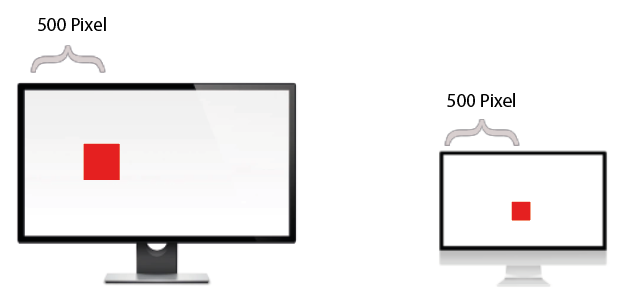
\includegraphics[scale=1]{pics/pixelDiff.PNG}
    \caption{Pixel-Unterschied}
\end{figure}

Aus diesem Grund können nicht einfach nur die rohen Koordinaten an alle Clients geschickt werden, sie müssen in Relation zu dem Bildschirm des Endgeräts und der Größe der Map, also dem Bild auf dem gerade gespielt wird, gesetzt werden.
(Dies ist nicht nur bei den Spieler-Koordintaten, sondern auch bei z.B. Items der Fall)
Der Code am Ende von jedem Draw-Zyklus sieht also so aus:

\begin{lstlisting}[,language=Java,label=lst:impl:socketIO]
    let transferX = (myPlayer.sprite.position.x - (windowWidth - ImageWidth) / 2) * originalBildBreite / neueBildBreite;
    let transferY = (myPlayer.sprite.position.y - (windowHeight - ImageHeight) / 2) * originalBildHoehe / neueBildHoehe;
    relPosData = {
      x: transferX,
      y: transferY
    }
    socket.emit('update', relPosData);
\end{lstlisting}

Im Server werden diese Koordinaten einfach zusammen mit der passenden ID des Players an alle Spieler verteilt:

\begin{lstlisting}[,language=Java,label=lst:impl:socketIO]

socket.on('update',updatePosition)

    function updatePosition(data) {
        let posData = {
            x: data.x,
            y: data.y,
            id: socket.id
        }
        // with socket.broadcast, everyone except the one who triggered the event gets the data
        socket.broadcast.emit('updatePosition', posData);
    }
\end{lstlisting}

Empfängt ein Client die Koordinaten, muss er diese dann wieder für sein Endgerät richtig umwandeln:


\begin{lstlisting}[,language=Java,label=lst:impl:socketIO]

socket.on('updatePosition',updatePosition);

    function updatePosition(data) {
        players[data.id].sprite.position.x = 
        data.x * neueBildBreite / originalBildBreite + (windowWidth - neueBildBreite) / 2;

        players[data.id].sprite.position.y = 
        data.y * neueBildHoehe / originalBildHoehe + (windowHeight - neueBildHoehe) / 2;
    }
\end{lstlisting}

Das Aktualisieren der Richtung des Sprites ist hingegen leichter. Dort spielt es keine Rolle, wie groß das Endgerät ist.
Beim Drücken von A oder D auf der Tastatur, wird einfach ein Event ausgelöst, dass die Richtung des Sprites bei jedem verbundenen Spieler ändert.


\begin{lstlisting}[,language=Java,label=lst:impl:socketIO]
    // A
    if (keyWentDown(65)) {
        socket.emit('updateDirection', 'left');
    }
    // D
    if (keyWentDown(68)) {
        socket.emit('updateDirection', 'right');
    }
\end{lstlisting}

Im Server wird die Information nun einfach an alle Clients verteilt:

\begin{lstlisting}[,language=Java,label=lst:impl:socketIO]
   socket.on('updateDirection',updateDirection);

   function updateDirection(data) {
    let dataWithId = {
        id: socket.id,
        direction: ""
    }
        if (data == "left") {
            dataWithId.direction = "left";
            socket.broadcast.emit('updateDirection', dataWithId);
        } else if (data == "right") {
            dataWithId.direction = "right";
            socket.broadcast.emit('updateDirection', dataWithId);
        }
}
\end{lstlisting}

Wird vom Client nun das <updateDirection>-Event empfangen, wird einfach die Orientierung des Sprites geändert.

\textbf{Synchronisieren von Projektilen oder Items} \\
Wenn ein Item aufgesammelt wird, soll dieses natürlich für die anderen Spieler nicht mehr verfügbar sein. Genauso soll, wenn eine Attacke ausgeführt wird, diese bei allen anderen Spielern auch ausgeführt werden.
Die Logik dazu ist relativ simpel. Jedes Item bekommt beim Erstellen eine eigene unique ID. Sammelt nun irgendein Spieler dieses Item auf, wird an den Server eine Benachrichtigung gesendet, dass jemand dieses Item aufgesammelt hat.
Dieser verteilt diese Information einfach an alle Spieler, und das Item mit der richtigen ID wird bei jedem gelöscht.
Bei den Projektilen ist es ähnlich. Wenn ein Spieler eine Attacke ausführt, wird auch das dem Server mitgeteilt. Der verteilt nun wieder die Information an alle Spieler, und bei jedem wird ein neues Projekil mit der gleichen ID erstellt.
Wenn irgendeiner der Spieler eine Kollision zwischen Player-Sprite und einem Projekil feststellt, wird das dem Server mitgeilt und dieser teilt wieder allen anderen Spielern mit, dass das Projektil bei jedem gelöscht werden muss.
Der Server hat einen Array mit Item-Objekten gespeichert. Vereinfacht sieht die Logik so auf der Server-Seite aus:

\begin{lstlisting}[,language=Java,label=lst:impl:socketIO]

    socket.on('deleteItem', deleteItem);
    socket.on('attack', syncAttacks);
    socket.on('deleteAttack', deleteAttack);

    function deleteItem(data) {
        items.forEach(i => {
            if (i == data.id) {
                // remove item from item array
                items.splice(items.indexOf(i), 1);
                socket.broadcast.emit('deleteItem', data);
            }
        });
    }

    // data consist of type of attack and attack ID
    function syncAttacks(data) {
        socket.broadcast.emit('attack', data);
    }

    // data consist of type of attack and attack ID
    function deleteAttack(data) {
        socket.broadcast.emit("deleteAttack", data);
    }

 \end{lstlisting}

Im Frontend werden einfach die bestimmten Events am richtigen Ort ausgelöst.
Zum Beispiel, wenn eine Bombe erstellt wird:

\begin{lstlisting}[,language=Java,label=lst:impl:socketIO]
    funciton addBomb() {
        // bomb gets created here
        let data = {
            playerId: socket.id,
            type: "bomb",
            x: bomb.position.x,
            y: bomb.position.y,
        }   
        socket.emit("attack",data);
    }
 \end{lstlisting}


Natürlich befindet sich auch die Logik, um die vom Server ausgelösten Events zu empfangen und darauf zu reagieren, am Client.

\begin{lstlisting}[,language=Java,label=lst:impl:socketIO]
    socket.on('deleteItem', syncItems);
    socket.on('attack', addAttack);
    socket.on('deleteAttack', deleteAttack);

    // remove item from the item array
    function syncItems(data) {
        items[data.index].remove();
        items.splice(items.indexOf(items[data.index]), 1);
    }

    // add a projectile, depending on the type of attack
    function addAttack(data) {
    switch (data.type) {
        case "default": addDefaultAttack(data);
            break;
        case "bomb": addBomb(data);
            break;
        case "blackHole": addBlackHole(data);
            break;
        case "piano": addPiano(data);
            break;
        case "mine": addMine(data);
            break;
        case "small": addSmall(data);
            break;
        }  
    }

    // delete the right projectile, depending on the type and the ID of the projectile
    function deleteAttack(data) {
        
        switch (data.type) {
            case "default":
                projectiles.forEach(p => {
                    if (p.id === data.id) {
                        p.remove();
                    }
                });
                break;
            case "bomb":
                bombs.forEach(b => {
                    if (b.id === data.id) {
                        b.remove();
                    }
                });
                break;
        // ... and so on
        }
    }

 \end{lstlisting}

Somit ist schon die meiste Logik des Servers gegeben. Was aber noch wichtiges fehlt, ist, dass wenn jemand aus der Spielumgebung fällt, immer auf Gewinner überprüft und Kills abgespeichert werden müssen.

\textbf{Tode und Kills} \\
Wie der Spieler in ScribbleFight gewinnt, wann er 'stirbt' und wie er Kills sammelt wird alles auf der Client-Seite in Kapitel \ref{impl:win} beschrieben.
Doch natürlich muss der Client auch mit dem Server kommunizieren, damit dieser alle diese Events auch an alle anderen Spieler mitteilen kann.
Stirbt ein Spieler, teilt er dies dem Server mit. Dieser speichert die Information ab und überprüft, ob der Spieler noch weiter mitspielen darf.
Ist er jedoch schon zum dritten Mal gestorben, ist dies nicht mehr der Fall und der Spieler wird aus der Spieler-Map vom Server gelöscht.
Ist ab dem Zeitpunkt nur mehr ein einziger Spieler in dem Map-Objekt gespeichert, hat dieser gewonnen.

\begin{lstlisting}[,language=Java,label=lst:impl:socketIO]
    function death(data) {
        players.get(data.deadPlayer).death++;
        if (players.get(data.deadPlayer).death >= 3) {
            // delete the player from player-map
            players.delete(data.deadPlayer);
            let transferData = {
                id: data.deadPlayer
            }
            // send the information that someone died to everyone
            io.emit('death', transferData);
            // disconnect the socket connection
            socket.disconnect();
        }
        // if player-map only has one player left, he has won 
        if (players.size <= 1) {
            socket.broadcast.emit("win");
        }
    }
 \end{lstlisting}

Der Client muss natürlich jetzt auf beide Events, also falls er gerade vom Spiel ausgeschieden wurde, oder gerade gewonnen hat, reagieren können.
Bekommt er die Benachrichtigung, dass gerade jemand ausgeschieden wurde, wird überprüft, ob es sich um ihn selbst handelt.
Falls ja, wird die draw-Methode gestoppt, ihm wird mitgeilt, dass er verloren hat und eine kurze Übersicht von seinen Spiel-Statistiken wird angezeigt.
Die Übersicht beinhaltet:
\begin{compactitem}
    \item Den Schaden, den er an alle anderen Spieler ausgeteilt hat
    \item Anzahl an Kills, die erzielt worden sind
    \item Der eigene Knockback, also ein Indikator wie oft der Spieler getroffen worden ist
\end{compactitem}
Falls es sich nicht um ihn handelt, passiert nichts.

\begin{lstlisting}[,language=Java,label=lst:impl:socketIO]
    socket.on('death',someoneDied);

    // data consits of id of dead player
    function someoneDied(data) {
    players[data.id].sprite.remove();
    if (data.id == myPlayer.id) {
        alert("You died!\n
        Your kills: " + myPlayer.kills + "\n" 
        + "Your damage: " + myPlayer.dmgDealt + "\n" 
        + "Your knockback: " + myPlayer.knockback);

        // stop the draw-function
        noLoop();
    }
}
 \end{lstlisting}

Bekommt der Spieler nun aber die Benachrichtigung, dass er gewonnen hat, wird diese Nachrichte ausgegeben und auch hier wird wieder eine kurze Übersicht der Spiel-Statistiken gezeigt.
Diesmal aber inklusive den Toden, da sie dieses Mal nicht mit Sicherheit drei sind.

\begin{lstlisting}[,language=Java,label=lst:impl:socketIO]
    socket.on('win',win);
     
    function win() {
        alert("You won!\n
        Your kills: " + myPlayer.kills + "\n" 
        + "Your damage: " + myPlayer.dmgDealt 
        + "\n" + "Your knockback: " + myPlayer.knockback 
        + "\n" + "Your deaths: " + myPlayer.death);
    }
 \end{lstlisting}

Wird im Client bestimmt, dass gerade ein Kill erzielt worden ist, speichert der Sever diese Information ab, damit sie immer abrufbar ist.
\begin{lstlisting}[,language=Java,label=lst:impl:socketIO]
    socket.on('kill',kill);
    
    // data consists of the id of the player who should get the kill
    function kill(data) {
        // player could leave before getting the kill
        if (players.get(data.damagedBy) != undefined) {
            players.get(data.damagedBy).kill += 1;
    }

 \end{lstlisting}

Nun hat der Server schon fast die ganze Funktionalität, die er benötigt, damit das Web-Game funktionert.
Das Einzige, was fehlt, ist dass der Server allen Spielern immer mitteilen muss, wann ein neues Item erscheinen soll.

\textbf{Item-Spawn-Event} \label{impl:itemSpawnB} \\
Items werden in ScribbleFight alle 10 Sekunden gespawned, falls ein Spieler mit dem Server verbunden ist.
Auf der Server-Seite ist das leicht umzusetzen. Mit der Methode \texttt{setIntervall()} kann einfach ein Intervall definiert werden, in dem eine Funktion ausgeführt werden soll.
Das Intervall wird auf 10 Sekunden gesetzt. Nun wird, solange ein Spieler vorhanden ist, alle 10 Sekunde ein Event ausgelöst, dass allen verbundenen Spielern mitteilt, wo, welche Art von Item erstellt werden soll.
Wie die x-Koodinaten berechnet werden, die für die Item-Spawns in Frage kommen, wird in Kapitel \ref{impl:xCoordinates} beschrieben.
Auf der Server-Seite sieht der Code also so aus:
\begin{lstlisting}[,language=Java,label=lst:impl:socketIO]
    setInterval(() => {
        // if players are connected with the server
        if (players.size > 0) {
            // get one of the available spawn points for items
            let x = getItemSpawnPoint();
            let data = {
                id: randomId(),
                x: x,
                num: getRandomInt(5)
            }
            // too many items on the field
            if (x != -1) {
                items.push(data.id);
            }
            // sending the event to every connected player
            io.emit('spawnItem', data);
        }
    }, 10000);

 \end{lstlisting}

Der Client muss jetzt nur mehr beim Empfangen dieses Events ein Item am richtigen Ort erstellen.
Wie Items am Client erstellt werden, findet kann in Kapitel \ref{impl:itemSpawnF} nachgelesen werden.\\
Vereinfacht sieht der Code am Client also so aus:


\begin{lstlisting}[,language=Java,label=lst:impl:socketIO]
    socket.on('spawnItem',createItem);

    // data consits of item-ID, type of item and position of item
    funciton createItem(data) {
        // item gets created here
    }
 \end{lstlisting}

Das waren allen Funktionalitäten des ScribbleFight-Web-Servers. Dieser läuft allerdings nicht mehr lokal, sondern auf einem Kubernetes-Cluster: Der Leocloud.
Wie der Server deployed werden konnte, wird in dem nächsten Kapitel beschrieben.


\section{Deployment [R]} \label{impl:Deployment}
\setauthor{Rafetseder Tobias}
Die Grundlage, um etwas auf einen Kubernetes-Cluster deployen zu können, ist ein Docker-Image. Näheres zu der Docker-Technologie wird in Kapitel \ref{tech:docker} beschrieben.
\subsection{Docker-Image [R]}
Da es sich bei dem Server, der für das Web-Spiel notwendig ist, nur um einen Web-Server, der statische Files hostet, handelt, und keine Datenbank nötig ist, ist das Docker-File relativ simpel.
\begin{figure}[H]
    \centering
    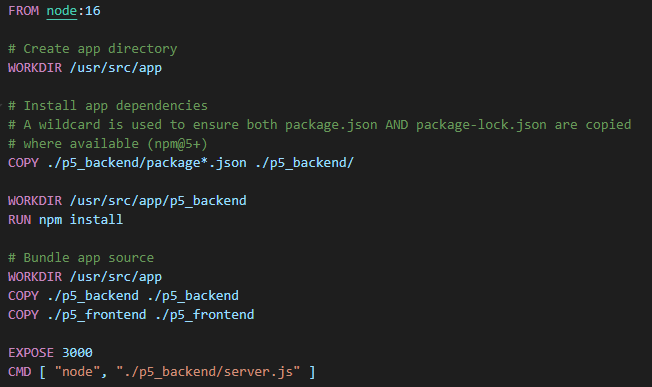
\includegraphics[scale=0.85]{pics/dockerfile_scribble.PNG}
    \caption{ScribbleFight Dockerfile}
\end{figure}
Die Zeilen Code werden im Folgenden genauer erläutert. \\
\begin{lstlisting}
    FROM node:16
\end{lstlisting}
Da Docker-Images von anderen Docker-Images erben können, wird nicht ein eigenes Base-Images verwendet, sondern das offizielle Node.js Image, das schon die Tools und Packages hat, die benötigt werden, um eine Node.js-Applikation auszuführen.
\\
\begin{lstlisting}
    WORKDIR /usr/src/app
\end{lstlisting}
Es wird ein neues Verzeichnis erstellt, von wo aus gearbeitet wird.
In diesem Verzeichnis werden alle folgenden Befehle ausgeführt. Der Vorteil davon ist, dass keine absoluten File-Paths benutzt werden müssen, sondern relativ zu diesem Verzeichnis relativ-Paths benutzt werden können. \\


\begin{lstlisting}
    COPY ./p5_backend/package*.json ./p5_backend/
\end{lstlisting}
Bevor \texttt{npm install} ausgeführt werden kann, muss das package.json File und package-lock.json File auf das Image kopiert werden.
Um das machen zu können, wird \texttt{COPY} benutzt. Dieser Befehl nimmt zwei Parameter: Source und Destination. Es werden package.json und package-lock.json in einen neuen Ordner des vorherig erstellen Arbeits-Verzeichnis kopiert. \\

\begin{lstlisting}
    WORKDIR /usr/src/app/p5_backend
    RUN npm install
\end{lstlisting}
Es wird nun das Verzeichnis, in das das package.json-und package-lock.json File kopiert worden sind, als Arbeits-Verzeichnis definiert.
Da dort diese Files vorhanden sind, kann \texttt{npm install} ausgeführt werden und alle nötigen Dependencies werden heruntegeladen. \\

\begin{lstlisting}
    WORKDIR /usr/src/app
    COPY ./p5_backend ./p5_backend
    COPY ./p5_frontend ./p5_frontend
\end{lstlisting}

Nun wird wieder das ursprüngliche Verzeichnis als Arbeits-Verzeichnis definiert. Dorthin werden die Files, die der Server zum Funktionieren braucht und auch die Files für das Frontend, die der Server hostet, kopiert. \\

\begin{lstlisting}
    EXPOSE 3000
    CMD [ "node", "./p5_backend/server.js" ]
\end{lstlisting}

Zuletzt wird nur mehr der Port, den der ScribbleFight-Server akzeptiert, nach aussen freigegeben, und mit dem Befehl \texttt{CMD} der Server gestartet. \cite{build_image}

\subsection{Leo-Cloud [R]}
Die Leo-Cloud ist eine Cloud-Computing-Umgebung der HTL Leonding.
Da nun ein funktionierendes Image des Web-Servers vorhanden ist, kann an dem Deployment an die Leo-Cloud gearbeitet werden.

Zuerst muss das Image, das für das Deployment verwendet werden soll, in das Docker-Registry der HTL Leonding geladen werden.
Dazu kann der Befehl \texttt{docker login registry.cloud.htl-leonding.ac.at} benutzt werden, um sich mit den eigenen Anmeldedaten dort einzuloggen.
Danach wird das Image einfach mit dem Befehl \texttt{docker push registry.cloud.htl-leonding.ac.at/t.rafetseder/<image-name>/<image-version>} hochgeladen.

Um das Deployment umzusetzten, werden drei YAML-Files benötigt.
YAML ist eine Daten-Serialisierungs-Sprache, die gerne benutzt wird, um Konfigurations-Files zu schreiben.

Diese drei Files sind:
\begin{compactitem}
    \item Deployment-File
    \item Service-File
    \item Ingress-File
\end{compactitem}

In dem Deployment-File kann die Konfigurationen zum eigentlichen Deployment festgelegt werden, zum Beispiel welches Image verwendet werden soll,
welche Anzahl an Pods (Linux-Containern) verwendet werden sollen, oder welcher Port benutzt werden soll.

\begin{figure}[H]
    \centering
    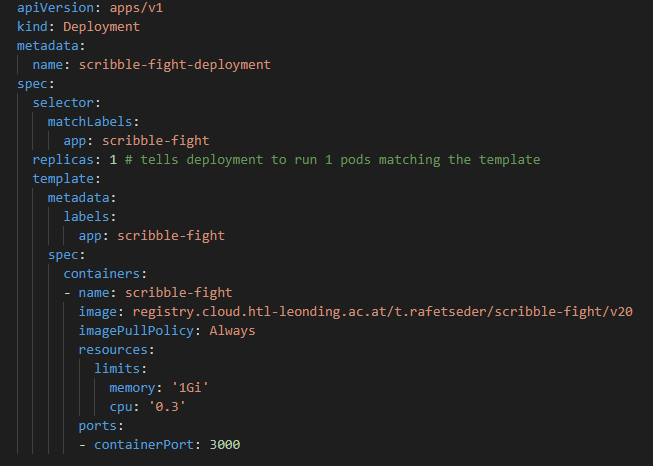
\includegraphics[scale=0.85]{pics/deployment.PNG}
    \caption{ScribbleFight Deployment.yaml}
\end{figure}

Auf einem Kubernetes-Cluster laufen viele Pods. Diese müssen in einer Weise verbindet werden. Das ist der Job von Service-Files.
Service abstrahiert die IP-Adresse eines Pods zu einem statischen Service-Name, sodass externe Requests zu multiplen Pods geleitet werden können.
\\
Das Weiterleiten von Requests zu dem erwünschten Pod basiert auf der \texttt{selector}-spec am Service, der mit dem Metadaten-Label des Pods zusammenpassen muss.

\begin{figure}[H]
    \centering
    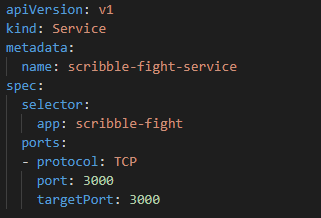
\includegraphics[scale=1]{pics/service.PNG}
    \caption{ScribbleFight Service.yaml}
\end{figure}

Zusätzlich muss noch konfiguriert werden, wie Services in einem Cluster via IP-Adresse oder URL erreicht werden können.
Dazu werden Ingress-Files verwendet. Ein Ingress ist eine Ansammlung von Regeln, die einkommende Verbindungen erlauben, Cluster-Servives zu erreichen.
Das Ingress-Spec-Field stellt einen Service-Namen und Service-Port bereit, der gemeinsam mit der URL-Route von dem Service exposed wird.

\begin{figure}[H]
    \centering
    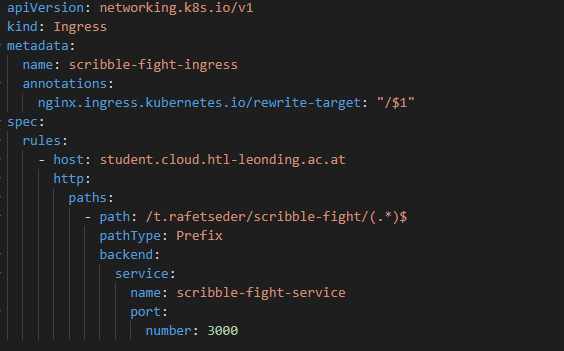
\includegraphics[scale=0.85]{pics/ingress.PNG}
    \caption{ScribbleFight Ingress.yaml}
\end{figure}



% Ben dein teil kommt hier herein


\newpage
\section{Map-Erkennung [H]}\label{maai:maperkennung:head}
Nachdem der Spieler der Lobby beigetreten ist, wird es Zeit für ihn die Spielumgebung zu zeichnen und diese für die
Abstimmung freizugeben. Das passiert, indem er oder sie einen QR-Code (``Quick Response''), welcher sich in der
Mitte der Lobby befindet, mit einem mobilen Endgerät, das über eine Kamera verfügt, abscannt. Somit wird
er auf eine Webseite geleitet, welche wieder auf die Kamera zugreift. Auf dieser ist bereits eine Objekterkennung
vorprogrammiert. Auf die Funktionsweise und auf die technische Umsetzung wird im folgenden eingegangen. Wenn der Spieler
merkt, dass die Objekterkennung das Blatt erkannt hat, kann dieser ein Bild aufnehmen. Im nächsten Schritt ist es nochmals möglich,
die erkannten Kanten zu verschieben. Wenn sich der User für das Foto als Map entscheidet, so kann er den ausgewählten Teil in eine
top-down-2d-Perspektive
umwandeln. Es werden also dabei die vier ausgewählten Ecken, welche über die Kanten des Blatt Papiers liegen,
für eine Perspektiven-Transformation
mit OpenCV2 herangezogen. Wenn der Spieler dann so weit ist, kann er dieses Bild beziehungsweise die Map bestätigen und
sendet sie somit zurück an die Lobby. Dann kann die Abstimmung beginnen.

\begin{figure}[H]
  \centering
  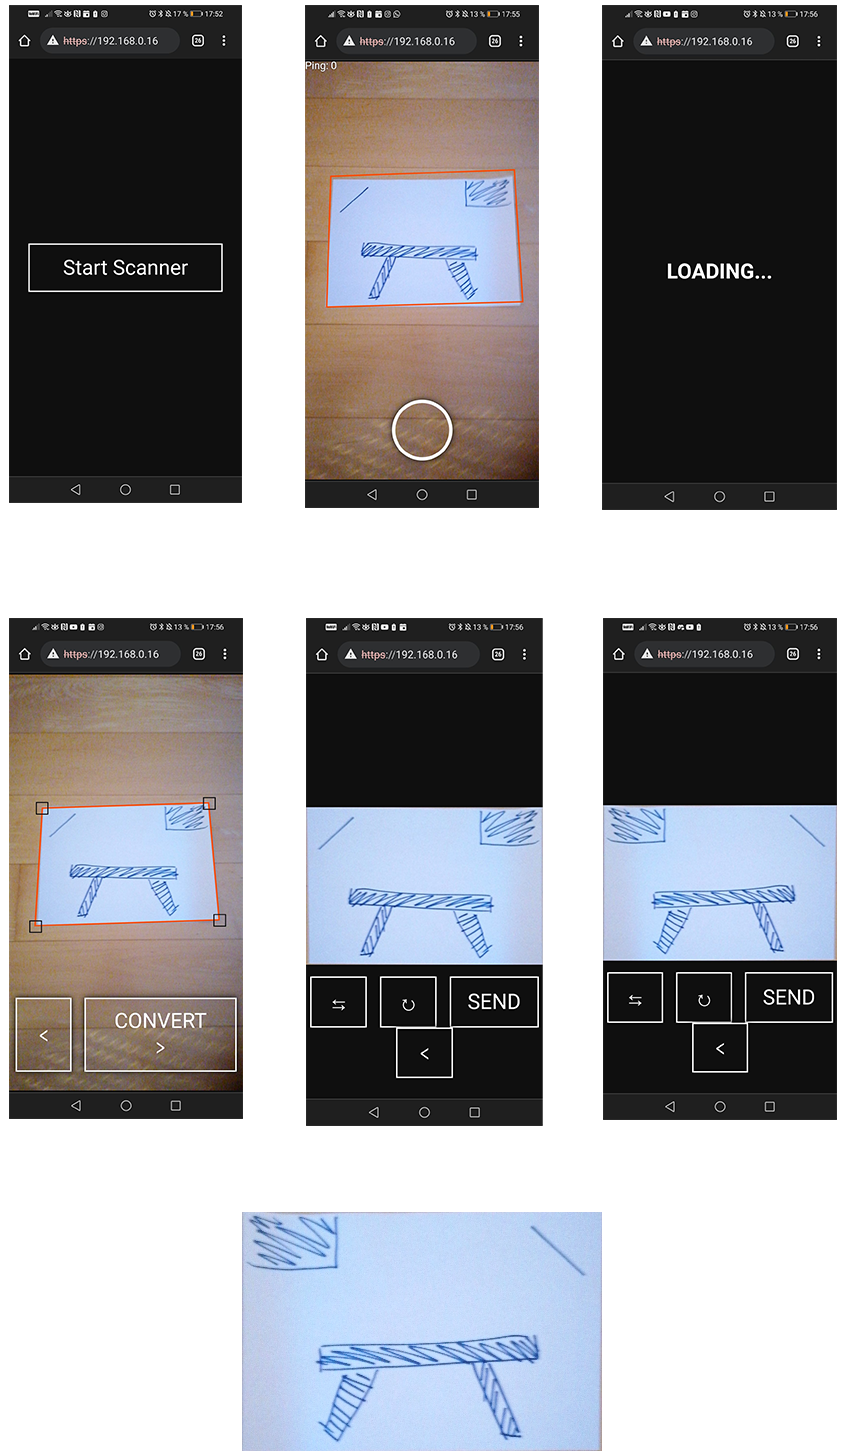
\includegraphics[scale=0.4]{pics/demo_maperkennung/sammlung_1.png}
  \caption{Screenshots der Maperkennungsanwenung}
  \label{fig:map:maperkennungsprozess}
\end{figure}

\setauthor{Himmetsberger Jonas}
\subsection{Objekterkennung [H]}
Das Thema ``Objekterkennung'' ist ein schnell wachsendes und sich verbesserndes Feld in der Welt der Bildverarbeitung beziehungsweise
Bildanalyse. \\
Die Objekterkennung ist ein großer Teil unserer Arbeit. Hier wird aus dem live Footage der Kamera das Blatt Papier und anschließend
in einer Aufnahme die Map erkannt.
\\
\\
Die Objekterkennung wird zum Beispiel bei komplexen und großen Paketdiensten eingesetzt. Sollen Pakete nach Farbe gruppiert werden, so
reicht bereits ein Farbsensor. Das ist in den meisten Fällen jedoch nicht genügend.
Vielmals werden Pakete auf Strichcodes oder Adressen überprüft.
Wenn also unterschieden werden muss, wo welches Paket landen soll, so ist eine Kamera nötig. Diese muss
ein genügend gut auflösendes Bild aufnehmen, dass daraus Informationen gewonnen werden können. Die Daten müssen zur Auswertung
mathematisch beschrieben werden. Zur Übersetzung werden Verfahren, wie Kantenerkennung, Transformationen oder Größen- und Farberkennung,
aber auch Künstliche Intelligenzen
eingesetzt. In dieser Arbeit wurden Kanten zur Objekterkennung herangezogen.
Die Korrektheit des Ergebnisses ist abhängig von der Korrektheit der bereitgestellten Daten und wie genau das Objekt mathematisch
beschrieben werden kann. \cite{objekterkennung}
\\
Ein weiteres Beispiel, wo Objekterkennung eingesetzt wird, sind in
Fahrerassistenzsysteme oder autonomes Fahren. Bereits in der ersten Stufe des autonomen Fahrens (dem assistierten Fahren),
werden zur Hilfe Kameras außerhalb des Fahrzeugs angebracht. In einem Auto, welches als Stufe eins autonomes Assistenzsystem
eingestuft wird, werden diese Kameras für einen automatischen Spurhalteassistenten eingesetzt. Via Bildanalyse und Objekterkennung
werden die Linien auf der Straße erkannt. \\
In höheren Stufen ist die Objekterkennung nicht mehr wegzudenken. Es müssen Verkehrsschilder und Personen auf der Straße erkannt
werden, um daraufhin entsprechend zu agieren. \cite{selfdriving}

Andere Beispiele:
\begin{compactitem}
  \item Gesichtserkennung, um das Smartphone zu entsperren.
  \item Qualitätskontrolle, zur Erkennung und automatischen Entfernung von kaputten oder beschädigten Teilen.
  \item Personenerkennung, um Menschenmassen zu analysieren.
\end{compactitem}

\subsubsection{Beschreibung der Funktionalität [H]}\label{maai:beschrFunktionalitaet}

Wie schon erwähnt können aus Bildern Daten erkannt werden. Viele Pixel bilden insgesamt ein Bild, welches visuell aufgenommen wird und in welchem alles Mögliche erkannt werden kann. Jeder einzelne dieser Pixel in einem digitalen Bild enthält Informationen über die Helligkeit und über die Farbe. Der Bildpunkt setzt sich zusammen aus den Farben Rot, Grün und Blau. Aus diesen drei können alle möglichen Farben abgebildet werden.
\\
Bevor darauf eingegangen wird wieso die Konturenerkennung als Art der Bilderkennung verwendet wurde, ist es noch entscheidend zu wissen, wie der Mensch Objekte erkennt.
\\
In dem menschlichen Auge passiert die Farberkennung via den Zapfen. Auch hier wird die Wellenlänge des Lichts in ein Gemisch aus Rot, Grün und Blau aufgeteilt. Allerdings wird das reine Farbsehen nicht benötigt, um Objekte zu erkennen. Es reicht schon, wenn nur Informationen über die Helligkeit empfunden werden. Somit künnen zum Beispiel auch in Schwarz-Weiß-Bildern, oder in der Dunkelheit bei wenig Licht, Objekte erkannt werden. Ein Mensch erkennt einen Unterschied zwischen Objekten, welche sich in einem dreidimensionalen Raum befinden leicht, indem das eine Objekt sich in der Helligkeit von dem anderen Objekt unterscheidet. Das heißt, dass wenn z.B. ein Würfel auf einem Boden liegt, ist dieser erkennbar, weil er anders viel Licht reflektiert als der Boden. An der Stelle, wo der Würfel aufhört, kann eine Kontur erkannt werden. Hier ist der Unterschied zwischen Boden und Würfel erkennbar. \cite{sehen}
\\
Und genau so passiert auch die Objekterkennung in dem Spiel ScribbleFight. Hier wird zuerst aus der Live-View, welche vom Client zur Verfügung gestellt wird, das Farbbild in Graustufen konvertiert. Das passiert, indem für jeden Pixel ein ``Durchschnitts-Wert'' der Helligkeit von allen drei Farbwerte (Rot, Grün, Blau), welche in einem 8-Bit System von 0 bis 255 geht, gebildet wird. Wie dies jedoch genauer funktioniert, wird im Kapitel Bildverarbeitungsalgorithmen
\ref{maai:alogs}
genauer erklärt.

\begin{lstlisting}[caption=Alle unnötigen Bilddaten entfernen,language=Python,label=lst:impl:filters]
    def check(img):
        
        ...

        imgGray = cv2.cvtColor(img, cv2.COLOR_BGR2GRAY) # CONVERT IMAGE TO GRAY SCALE
        imgBlur = cv2.GaussianBlur(imgGray, (5, 5), 1)  # ADD GAUSSIAN BLUR
        upperThres = 40
        lowerThres = 40
        imgThreshold = cv2.Canny(
            imgBlur, upperThres, lowerThres)  # APPLY CANNY BLUR
        
        ...
\end{lstlisting}


Nachdem das Bild in ein Schwarz-Weiß-Bild umgewandelt wurde, muss vor der Konturenerkennung noch ein Schwellwert-Bild eines unscharfen Bildes erzeugt werden.
Das dritte Bild von links, oben in der Abbildung \ref{fig:map:documentscanner}. Das Schwellwert-Bild dient dazu, maximal viel Information aus dem Bild zu entfernen. Somit bleiben nur die relevanten Informationen übrig, welche OpenCV2 braucht um Konturen bilden zu können.\\
\\
\begin{lstlisting}[caption=Erhalten von Konturen,language=Python,label=lst:impl:getContours]
        ...

        contours, hierarchy = cv2.findContours(
            imgThreshold, cv2.RETR_LIST, cv2.CHAIN_APPROX_SIMPLE)  # FIND ALL CONTOURS

        # FIND THE BIGGEST COUNTOUR
        accuracy = 25/1000
        area = 1000
        biggest, maxArea = biggestContour(
            contours, accuracy, area)  # FIND THE BIGGEST CONTOUR

        ...

        edges = getEdges(oldBiggest, biggest, contours, img, biggestChanged)

    return edges
\end{lstlisting}

In diesem Code-Block ist ersichtlich, wie OpenCV2 die Konturen aus einem Schwellwert-Bild extrahiert,
und danach die größte herausfindet.
Wie die Funktion ``biggestContour(\dots)'' funktioniert ist in diesem Codeblock \ref{lst:impl:findBiggestContour} beschrieben. Danach wird in ``getEdges(\dots)'' ein Numpy-Array von den Eckpunkten erzeugt, in eine anderer Reihenfolge, welche für den Perspektiven Transform relevant ist, umgewandelt und dann als Return-Wert zurückgegeben.

\begin{figure}[H]
  \centering
  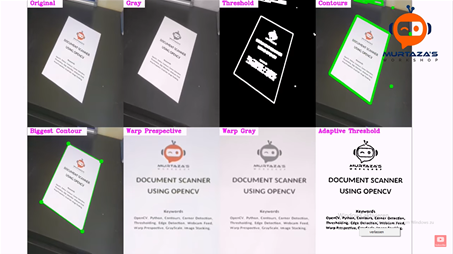
\includegraphics[scale=1]{pics/maperkennung/documentscanner.png}
  \caption{Documenten Scanner \cite{maai:documentscannerYoutube:cite}}
  \label{fig:map:documentscanner}
\end{figure}

Aus diesen Konturen, welche OpenCV2 erkennt, wird die größte, geschlossene Umrandung herausgesucht. Es wird davon ausgegangen, dass sich hier das fokussierte Objekt, also das Blatt Papier, befindet. Um nun die vier Eckpunkte lokalisieren zu können, wird eine vorgefertigte Funktion namens ``approxPolyDP'' angewendet. Diese legt, mit den übergebenen Parametern, ein Viereck über die Konturen. Danach werden aus diesem Viereck die 4 Eckpunkte extrahiert und als Array wieder an den Client zurückgesendet.


\begin{lstlisting}[caption=approxPolyDP,language=Python,label=lst:impl:findBiggestContour]
    def biggestContour(contours, accuracy, areaVal):  # FIND THE BIGGEST CONTOUR
        biggest = np.array([])
        max_area = 0

        for i in contours:
            area = cv2.contourArea(i)
            if area > areaVal:
                peri = cv2.arcLength(i, True)
                # findet die vier Eckpunkte heraus und gibt diese zurueck
                approx = cv2.approxPolyDP(i, accuracy * peri, True)
                if area > max_area and len(approx) == 4:  # IF == 4 THEN SQUARE
                    biggest = approx
                    max_area = area
        return biggest, max_area
\end{lstlisting}

In der folgenden Funktion namens ``getWrappedImg(\dots)'', wird das Bild, welches aufgenommen wurde, in eine zwei-dimensionale top-down Ansicht umgewandelt. Allerdings geschieht dies nur da, wo zuerst die Eckpunkte beziehungsweise das Blatt Papier (also die Spielumgebung) gefunden wurden. Wie dies funktioniert ist im folgenden Codeblock
\ref{lst:impl:convertPoints} ersichtlich.


Zuerst wird aus dem übergebenen ``snipset''-Parameter, welcher als Array vorliegt, die Daten ausgelesen und auf die Variablen ``pt\_A'' bis ``pt\_D'' geschrieben. Diese vier Buchstaben geben die Eckpunkte an. Aus diesen Eckpunkten wird im Folgenden dann ein Vektor erzeugt. Für weitere Berechnungen wird dann noch die Länge zwischen den wahrscheinlich parallel zueinanderliegenden Vektoren AD und BC berechnet. Dies ist wichtig, um im späteren Code herauszufinden, in welcher Orientierung das Blatt Papier zu der Kamera liegt.

\begin{lstlisting}[caption=Bild in Vogelperspektive umwandeln,language=Python,label=lst:impl:convertPoints]
def getWrappedImg(img, snipset):
    snipset = squarify(snipset)

    pt_A = snipset[0]
    pt_B = snipset[1]
    pt_C = snipset[2]
    pt_D = snipset[3]

    lineAB = np.array([pt_A, pt_B])
    lineBC = np.array([pt_B, pt_C])
    lineCD = np.array([pt_C, pt_D])
    lineDA = np.array([pt_D, pt_A])

    width_AD = np.sqrt(((pt_A[0] - pt_D[0]) ** 2) + ((pt_A[1] - pt_D[1]) ** 2))
    width_BC = np.sqrt(((pt_B[0] - pt_C[0]) ** 2) + ((pt_B[1] - pt_C[1]) ** 2))
\end{lstlisting}
Im folgenden Code-Block wird zuerst im Grunde genommen genau dasselbe ausgeführt, wie im zuvor erklärtem Code-Block \ref{lst:impl:convertPoints}. Hier wird die größere Länge der beiden Vektoren AB und CD, welche wahrscheinlich in der Realität parallel zueinander liegen, errechnet. Dabei wird angenommen, dass diese beiden Längen die Höhe des Blatt Papiers sind.
\begin{lstlisting}[language=Python,label=lst:impl:findBiggestLine,firstnumber=16]
    maxHeight = max(int(width_AD), int(width_BC))
    if maxHeight == width_AD:
        lineA = lineDA
    else:
        lineA = lineBC

    height_AB = np.sqrt(((pt_A[0] - pt_B[0]) ** 2) +
                        ((pt_A[1] - pt_B[1]) ** 2))
    height_CD = np.sqrt(((pt_C[0] - pt_D[0]) ** 2) +
                        ((pt_C[1] - pt_D[1]) ** 2))
    maxWidth = max(int(height_AB), int(height_CD))
    if maxWidth == height_AB:
        lineB = lineAB
    else:
        lineB = lineCD
\end{lstlisting}

Die errechnete maximale Höhe wird noch mit einem realistischen Faktor multipliziert, um ein akkurateres Ergebnis der Perspektiventransformation erzielen zu können. Dieser ``realistische Faktor'' wird errechnet, indem der Winkel zwischen den beiden größten orthogonal zueinander liegenden Linien in folgende Formel miteinbezogen wird:
\[ factor
  = \dfrac{90}{(180-angle)}
\]
Dieser errechnete Faktor staucht die Höhe eines Bildes, welches von der unteren Blattkante aufgenommen wurde und streckt die Höhe von jene, welche von oben Blattkante aufgenommen wurden.


\begin{lstlisting}[language=Python,label=lst:impl:angle,firstnumber=31]
    angle = ang(lineA, lineB)
    if angle == 90:
        factor = 1
    if angle > 90:
        factor = 90 / (180-angle)
    if angle < 90:
        factor = 90 / angle

    maxHeight *= factor
\end{lstlisting}

Im letzten Teil der Funktion wird das Bild in die richtige Perspektive transformiert. Dies wird erzielt, indem die beiden vorgefertigten Funktionen ``cv2.getPerspectiveTransform(\dots)'' und ``cv2.warpPerspective(\dots)'' verwendet werden. Als Return-Wert liefert die genannte Funktion ein Bild mit dem Datentypen OpenCV2, welches dann im späteren Verlauf noch umcodiert werden muss.

\begin{lstlisting}[language=Python,label=lst:impl:wrapPerspective,firstnumber=40]
    m = np.array([pt_A, pt_B, pt_C, pt_D])
    m = rotateCW(m)
    input_pts = np.float32(m)
    output_pts = np.float32([[0, 0],
                            [0, maxHeight - 1],
                            [maxWidth - 1, maxHeight - 1],
                            [maxWidth - 1, 0]])

    M = cv2.getPerspectiveTransform(input_pts, output_pts)

    dst = cv2.warpPerspective(
        img, M, (int(maxWidth), int(maxHeight)), flags=cv2.INTER_LINEAR)

    return dst
\end{lstlisting}

Das Wissen, welches dazu benötigt wurde, diesen Programmcode zu schreiben entspringt aus einer Video-Erklärung auf der Plattfrom ``YouTube'' namens ``Document Scanner OPENCV PYTHON | Beginner Project.'' des Kanals ``Murtaza's Workshop - Robotics and AI''. \cite{maai:documentscannerYoutube:cite}

\subsection{Open-CV2 [H]}
\subsubsection{Bildverarbeitungsalgorithmen} \label{maai:alogs}

Bildverarbeitungsalgorithmen sind Grundbausteine für die Bild- beziehungsweise Map-Erkennung. Ohne diesen können keine, oder nur wenige Daten aus Bildern ausgelesen werden. Somit würde jedes Bild nur Informationen über die Helligkeit und die Farbe/Farbhelligkeit jedes Bildpunktes beinhalten. Deshalb ist es wichtig Bildverarbeitungsalgorithmen zu verwenden um mehr Informationen aus den Bildern, welche dem Python-Server zur Verfügung gestellt werden, zu erkennen und zu erhalten. In dieser Arbeit wurden folgende Methoden von OpenCV2 verwendet, welche das Erkennen des Blatt Papiers ermöglichten. Im Folgenden wird näher auf die Funktionsweise der einzelnen Algorithmen eingegangen. Diese sind:

\begin{compactitem}
  \item cv2.cvtColor(image, cv2.COLOR\_BGR2GRAY) (``Grayscaling''): Diese Funktion bewirkt eine Graustufenkonvertierung eines gegebenen Bildes.
  \item cv2.GaussianBlur(\dots) (``Blurring''): Mit dieser Funktion wird ein gegebenes Bild unscharf gezeichnet und somit unnötig genaue Informationen entfernt.
  \item cv2.adaptiveThreshold(\dots) (``Adaptive Thresholding''): Hier wird die Schwellwertbildung adaptiv festgelegt. Es wird das gegebene Bild in Raster unterteilt und für jeden dieser Raster ein Schwellwert gebildet. Somit werden Farbübergänge eliminiert und es kommt ein reines Schwarz-Weiß-Bild mit harten Kanten heraus.
  \item cv2.canny(\dots) (``Canny'' Kantenerkennung): Die Kantenerkennung liefert automatisch erkannte Kanten aus einem gegebenen Bild.
  \item cv2.approxPolyDP(\dots) (``ApproxPolyDP''): Diese Funktion vergröbert die erkannten Konturen um einen angegebenen Grad. Die erkannten Konturen werden auf wenige Punkte minimiert. Somit kann zum Beispiel über eine Kontur ein Vieleck gelegt werden.
  \item cv2.warpPerspective(\dots) (Perspektiven-Korrektur): Mit ``wrapPerspective'' kann ein Bild, welches in der dritten Dimension aufgenommen wurde und somit einer Perspektive unterlag Perspektiven-korrigiert werden.
\end{compactitem}

Nur einige der verwendeten Bildbearbeitungsalgorithmen sind basierend auf Pixelmanipulation. Andere Algorithmen, wie zum Beispiel ``ApproxPolyDP'', sind reines Auslesen von Bildwerten beziehungsweise -daten, welche durch Vorarbeit extrahiert wurden. \cite{opencvdocs}


\subsubsection{Grayscale}\label{maai:grayscale}
Die Quelle zu folgendem Unterabschnitt ist eine Erklärung der Graustufenbildung von ``Wikipedia.org'' \cite{grascale:cite}

Beim ``grayscaling'' werden Informationen über die Lichtintensität aus den einzelnen Pixeln extrahiert und über eine Gewichtung der drei Farben Rot, Grün und Blau gleichmäßig gewertet. Somit entsteht ein Bild, welches rein Informationen über die Helligkeit/Lichtintensität enthält.

Die Lichtintensität ist die Menge an Licht(stärke) pro Pixel. Diese Lichtstärke kann in einem 8-Bit System von den Farben Rot, Grün und Blau von 0-255 reichen. Der Kontrast geht somit von ganz schwarz, was einer Lichtintensität von 0 entspricht (es wird aus diesem Pixel kein Licht emittiert), bis ganz weiß, was in einem 8-Bit System 255 entspricht.

Für eine Umwandlung eines Bilds in dessen Graustufen wird für jeden Pixel also die Lichtintensität der drei Farben (Rot, Grün und Blau) beziehungsweise der Farbkombination dieser drei Farben gemessen und über eine Gewichtung der drei Werte ein ``Mittelwert'' errechnet. Diese Gewichtung kann über verschiedene Faktoren erfolgen. Daher ist es nicht gegeben, dass auch OpenCV2 die folgende Formel zur Umrechnung eines Bildes, welches aus einem RGB(A)-Farbraum (Rot (R); Grün (G); Blau (B); Opazität (A)) in Graustufen konvertiert werden soll, verwendet. Die Formel dient deswegen nur als Exempel, um alle drei Werte auf eine lineare Gleichgültigkeit für das menschliche Auge zu setzen, um somit ein Graustufenbild zu erzeugen:

\[
  Y_{ linear } = 0,2126 * R_{ linear } + 0.7152 * G_{ linear } + 0.0722 * B_{ linear }
\]

Aus dieser Formel ist erkennbar, dass die Farbe Grün mehr gewichtet wird als Rot und Blau. Dies resultiert daraus, dass das Auge die meiste Lichtinformation aus der Farbe Grün extrahieren kann. Somit wirkt auch diese Farbe am hellsten für das menschliche Auge. Deshalb wird sie am höchsten gewichtet, damit ein scheinbar ausgeglichener Wert der Lichtintensität der Farbkombination der drei Farben herauskommt. Dieser gewichtete Wert (Y), welcher auch als Luminanz bezeichnet wird, ist die Basis für die Graustufenkonvertierung.

Im folgendem Code-Beispiel \ref{maai:grayscaling} wird die Umsetzung einer Graustufenkonvertierung mittels OpenCV2 in der Programmiersprache Python gezeigt.
% Quelle: https://en.wikipedia.org/wiki/Grayscale

\begin{lstlisting}[caption=Graustufenkonvertierung,language=Python,label=maai:grayscaling]
    # OpenCV2 used as pixel manipulation library
    import cv2
  
    # read Image from Folder
    image = cv2.imread('Path/to/your/image.jpg')
    # Convert RGB image to (2) gray
    gray = cv2.cvtColor(image, cv2.COLOR_BGR2GRAY)
    
    # display the original image (input) on the screen
    cv2.imshow('Original image',image)
    # display the grayscaled image (output of cv2 funktion cvtColor) on the screen
    cv2.imshow('Gray image', gray)
      
    cv2.waitKey(0) # waits until a key is pressed
    cv2.destroyAllWindows() # destroys the window showing image
\end{lstlisting}
%Quelle: Zitat: https://docs.opencv.org/3.4/d8/d01/group__imgproc__color__conversions.html

Dieses Stück Programmcode führt zu folgendem Ergebnis:

\begin{figure}[htb]
  \centering
  \begin{minipage}[t]{0.45\linewidth}
    \centering
    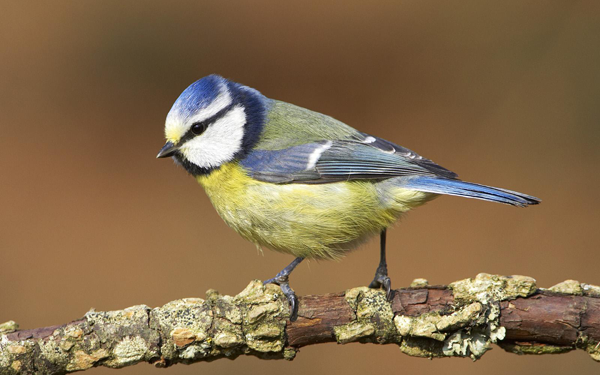
\includegraphics[width=\linewidth]{pics/bildverarbeitungsalgos/input.png}
    \caption{Input \cite{maai:input:cite}}
    \label{maai:grayscaling:input}
  \end{minipage}
  \hfill
  \begin{minipage}[t]{0.45\linewidth}
    \centering
    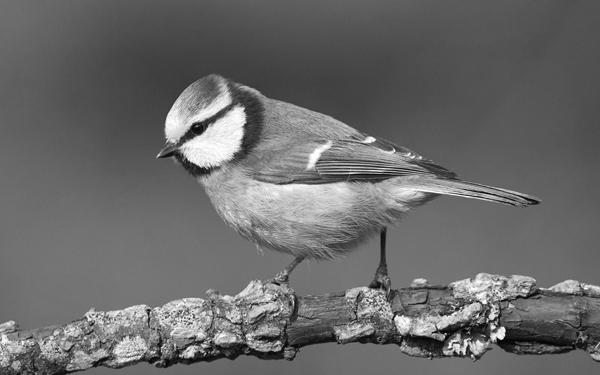
\includegraphics[width=\linewidth]{pics/bildverarbeitungsalgos/grayscaling_output.png}
    \caption{Output}
    \label{maai:grayscaling:output}
  \end{minipage}
\end{figure}
%Quelle: https://s3.envato.com/files/16109405/index.html

\subsubsection{Blurring}\label{maai:blurring}
Die Quelle zu folgendem Unterabschnitt ist eine Erklärung wie man Bilder weichzeichnet von``Akeyla Pradia Naufal'' \cite{blurring:cite}

Soll ein Bild ``geblurred'' (engl. für verwischen/verschwommen) werden, so ist das Ziel eine Unschärfe. Ähnlich, wie das ``Grayscaling'' ist auch das unscharf Zeichnen eines Bildes reine Pixelmanipulation. Hier wird jedoch nicht ein einzelner Pixel zur Berechnung der Unschärfe herangezogen, sondern eine zweidimensionale Matrix an umliegenden Bildpunkten. Somit wird jeder Pixel basierend auf dessen benachbarten Bildzellen manipuliert.

Um eine Unschärfe zu erzielen, muss eine mathematische Operation der Faltung einer spezialisierten Matrix, genannt Kernel, auf die Matrix des Bildes angewandt werden. Dabei wird diese Faltungsoperation auch ``Konvolution'' genannt.

Mathematisch gesehen ist Konvolution, also die Faltung zweier Matrizen, A mit der Größe a \(\times\) b und B mit der Größe c \(\times\) d, eine \((a + c -1) \times (b + d - 1)\) Matrix C mit folgenden Einträgen:
\[
  C_{ rs } = \sum_{i+k=r+1, j+l=s+1}^{r=a+c-1,s = b + d - 1} A_{ ij }B_{ kl }
\]
Aus dieser Formel ist ersichtlich, dass das Falten beziehungsweise die Konvolution zweier Matrizen A und B eine neue Matrix C erzeugt. In dieser werden die Einträge durch die Summe des Produkts der Einträge der Matrix A mit den am gleich liegenden zweidimensionalen Index entsprechenden Einträgen der anderen Matrix B gebildet. Alle diese Produkte werden im Zweidimensionalen, also entlang den Zeilen und Spalten, berechnet.

Der zuvor genannte (Begriff) Kernel kann als Matrix beschrieben werden. Diese dient dazu ein Bild in dessen Aussehen zu verändern. Somit ist der Begriff nicht nur auf das Weichzeichnen von Bildern begrenzt. Ein Kernel kann zum Beispiel auch dazu verwendet werden, um Kanten in Bildern zu schärfen.

Da der Kernel eine Matrix mit einem Mittelpunkt ist, muss die Kernel Größe einer ungeraden Zahl, zum Beispiel \([5*5]\), entsprechen.

In dieser Diplomarbeit wurde häufig der ``Gauß'sche'' Weichzeichnungsfilter verwendet. Dieser Filter gibt jedem Bildpunkt, welche um einen betrachteten Pixel liegen, eine Gewichtung.

Diese Gewichtung nimmt mit der Distanz zu dem betrachteten Pixel ab. Somit hat theoretisch jeder Pixel in der Bild-Matrix eine eigene Gewichtung. Da diese jedoch mit der Distanz so stark abnehmen werden diese nicht mehr berücksichtigt. Die theoretische Formel zur Berechnung der Gewichte der Pixelwerte rund um einen fokussierten Bildpunkt sieht wie folgt aus:
\[
  G(x,y)=\frac{ 1 }{ 2*\pi*\sigma^2 }*e^{ - \frac{ x^2 + y^2 }{ 2*\sigma^2 } }
\]
Wobei x und y der horizontale und vertikale Abstand zum untersuchten Bildpunkt ist. Sigma ist die Standardabweichung (je höher der Wert von Sigma, desto stärker ist auch der Weichzeichnungseffekt).

In der Realität werden jedoch die Werte dieser ``Gaus'schen'' Funktion mittels der Werte im Kernel genähert. Dabei macht es wenig Sinn, dass die Kernel-Matrix groß gewählt wird, da der Wert eines Eintrags im Kernel mit der Distanz zum Mittelpunkt abnimmt. Dabei wird oft das \(\sigma\) der Funktion in der Programmierung ignoriert und vom Programm auf Basis der angegebenen Größe des Kernels selbst entschieden. Somit sieht eine Näherung an die ``Gaus'sche'' Formel durch eine Kernel Matrix wie folgt aus:
\[
  \frac{ 1 }{ 16 } * \left[\begin{array}{rrr}
      1 & 2 & 1 \\
      2 & 4 & 2 \\
      1 & 2 & 1 \\
    \end{array}\right]
\]
OpenCV2 stellt jedoch bereits Funktionen zur Verfügung, welche das Kalkulieren des Kernels abnimmt. Im folgendem Codeblock (\ref{maai:gaussianblur}) wird gezeigt, wie diese Funktion in dieser Arbeit verwendet wurde.

% Quelle: https://medium.com/swlh/how-image-blurring-works-652051aee2d1

\begin{lstlisting}[caption=Gaussian Blur,language=Python,label=maai:gaussianblur]
    import cv2
    import numpy
    
    # read image
    src = cv2.imread('/path/to/image.png', cv2.IMREAD_UNCHANGED)
    
    # apply guassian blur on src image
    # (10,10) is the Kernel size
    dst = cv2.GaussianBlur(src,(10,10),cv2.BORDER_DEFAULT)
    
    # display input and output image
    cv2.imshow("Gaussian Smoothing",numpy.hstack((src, dst)))
    cv2.waitKey(0) # waits until a key is pressed
    cv2.destroyAllWindows() # destroys the window showing image
\end{lstlisting}

%Quelle: https://www.tutorialkart.com/opencv/python/opencv-python-gaussian-image-smoothing/

Wird der Programmcode ausgeführt, so erzeugt dieser folgenden Effekt:

\begin{figure}[htb]
  \centering
  \begin{minipage}[t]{0.45\linewidth}
    \centering
    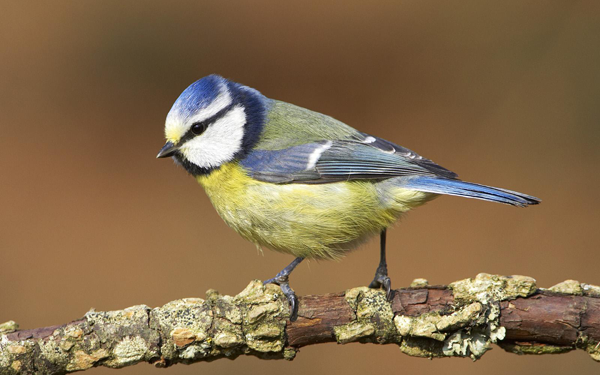
\includegraphics[width=\linewidth]{pics/bildverarbeitungsalgos/input.png}
    \caption{Input \cite{maai:input:cite}}
    \label{maai:gaussianblur:input}
  \end{minipage}
  \hfill
  \begin{minipage}[t]{0.45\linewidth}
    \centering
    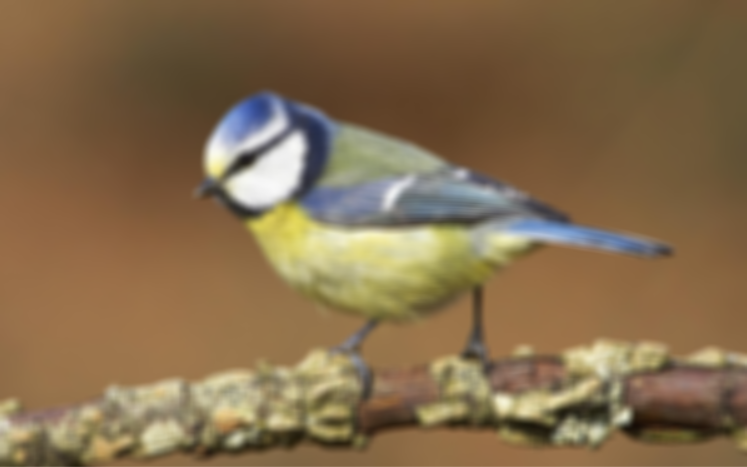
\includegraphics[width=\linewidth]{pics/bildverarbeitungsalgos/gaussianblur_output.png}
    \caption{Output}
    \label{maai:gaussianblur:output}
  \end{minipage}
\end{figure}

% Quelle: https://www.tutorialkart.com/opencv/python/opencv-python-gaussian-image-smoothing/

\subsubsection{Thresholding}
Die Quelle zu folgendem Unterabschnitt ist eine Erklärung wie man ein Schwellwert-Bild erzeugt von dem ``YouTube-Kanal'' ``Apeer\_micro'' \cite{thresholding:cite}

Das ``Image-Thresholding'' also die Schwellwertbildung eines Bilds ist basierend auf die ``Image-Segmentation''. Diese erzeugt eine Unterteilung eines Bildes in mehrere Segmente.

Das ``Image-Thresholding'' ist eine einfache Form der Segmentierung. Das ``Thresholding'' basiert auf gesetzte Schwellwerte, welches unterschiedlich ``intensive'' Pixel trennen soll. Dadurch ist das Produkt ein binäres Bild, welches aus Nullen und Einsen besteht (= entweder hell oder dunkel).

``Thresholding'' ist, wie auch die Graustufenkonvertierung (Kapitel ``Grayscaling'' \ref{maai:grayscale}), das Weichzeichnen von Bildern (Kapitel ``Blurring'' \ref{maai:blurring}) und viele andere Methoden der Bildverarbeitung, eine Art der Pixelmanipulation. Die Pixel sollen beim ``Image-Thresholding'' beziehungsweise bei der Schwellwertbildung so angepasst werden, dass Bilder und deren Pixel einfacher zu analysieren sind. In dieser Arbeit legte das Schwellwert-Bild den Grundbaustein zur Konturen-/Kantenerkennung.

Ziel ist es, aus einem Farb- beziehungsweise Graustufenbild eine Segmentierung zu erzeugen. Durch dieses Verfahren wird, wie zuvor erwähnt, ein binäres Bild erzeugt, welches nur noch Schwarz- und Weißwerte beinhaltet. Dies wird zum Beispiel dafür verwendet, dass ein Hintergrund vom Vordergrund getrennt wird. Somit werden sogenannte ``Regions Of Interest'' erkannt. ``Region Of Interest'' bedeutet ``Bereich von Interesse''. Hierzu werden spezielle Bereiche aus einem Histogramm, also einer Messkurve, ausgewertet beziehungsweise ausgewählt und nach dem zuvor definierten Schwellwert in Gruppen unterteilt. Somit gibt die ``Region Of Interest'' die fokussierten/für die Auswertung Interessanten Bereiche eines Bildes wieder. Dem Hintergrund wird in einem binären Bild der Wert 0 (null) zugewiesen und dem Vordergrund der Wert 1. Diese Werte werden in einem Bild als 0 (null) - schwarz und als 1 – Weiß dargestellt.

Durch das ``Thresholding'' gibt es die Möglichkeit ein Histogramm zu erstellen, um die Helligkeitswerte eines Bildes zu analysieren. Ein aus dem Graustufenbild (\ref{maai:thresholding:input}) erzeugtes Histogramm (\ref{maai:thresholding:histogramm}) sieht wie folgt aus:

\begin{figure}[htb]
  \centering
  \begin{minipage}[t]{0.45\linewidth}
    \centering
    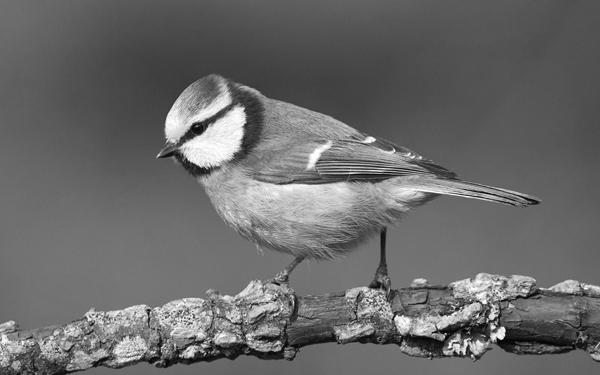
\includegraphics[width=\linewidth]{pics/bildverarbeitungsalgos/grayscaling_output.png}
    \caption{Input}
    \label{maai:thresholding:input}
  \end{minipage}
  \hfill
  \begin{minipage}[t]{0.45\linewidth}
    \centering
    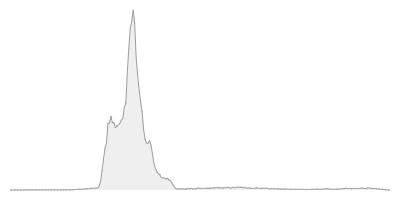
\includegraphics[width=\linewidth]{pics/bildverarbeitungsalgos/thresholding_histogram.png}
    \caption{Helligkeitsverteilung}
    \label{maai:thresholding:histogramm}
  \end{minipage}
\end{figure}

Das Histogramm veranschaulicht die Helligkeitsverteilung aller Pixel von den Werten 0 (null) (schwarz), welcher der Wert ganz links auf der X-Achse im Histogramm ist, bis 255 (weiß), welches dem äußersten X-Wert entspricht. Auf der Y-Achse befindet sich die Häufigkeit der vorkommenden Pixel mit der entsprechenden Helligkeit.
Es kann also erkannt und analysiert werden, dass überwiegend Hintergrund (dunkle Helligkeitswerte) in diesem Bild existiert. Damit aus dem Histogramm auch ein Schwellwert-Bild (das binäre Bild) erzeugt werden kann, wird ein zuvor definierter Schwellwert zur Verarbeitung der Pixel herangezogen. Somit werden global (!) nur alle Pixel über einem gewissen Helligkeitswert in den Wert 1 (Vordergrund) umgewandelt. Alle anderen bleiben Schwarz. In folgendem Bild (\ref{maai:thresholding:output}) an, kann durch die Schwellwertbildung erkannt werden, dass sich das interessante Objekt in der Bildmitte befindet:


\begin{figure}[htb]
  \centering
  \begin{minipage}[t]{0.45\linewidth}
    \centering
    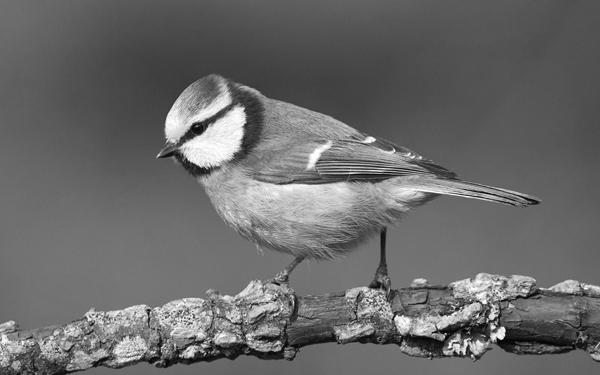
\includegraphics[width=\linewidth]{pics/bildverarbeitungsalgos/grayscaling_output.png}
    \caption{Input}
    \label{maai:thresholding:input:second}
  \end{minipage}
  \hfill
  \begin{minipage}[t]{0.45\linewidth}
    \centering
    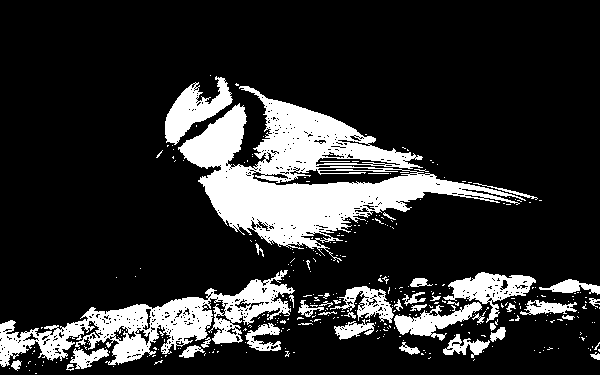
\includegraphics[width=\linewidth]{pics/bildverarbeitungsalgos/thresholding_output.png}
    \caption{Output}
    \label{maai:thresholding:output}
  \end{minipage}
\end{figure}
%Quelle: https://www.youtube.com/watch?v=8TkligJJCAQ&ab_channel=Apeer_micro
%Quelle: https://datacarpentry.org/image-processing/07-thresholding/


Für dieses Bild wurde ein globaler Schwellwert verwendet. Dies ist jedoch keine gute Entscheidung, wenn der Helligkeitseinfall im Bild unterschiedlich stark ist. Deshlab kann ein adaptiver Schwellwert zum Einsatz kommen. Dieser wird somit durch einen Algorithmus für einen Pixel basierend auf einem kleinen Bereich um ihn herum gebildet. Dadurch werden unterschiedliche Schwellwerte in unterschiedlichen Regionen des Bildes gebildet, um eine ungleichmäßige Beleuchtung zu korrigieren.

%Quelle: https://docs.opencv.org/4.x/d7/d4d/tutorial_py_thresholding.html
Programmiertechnisch wurde dies wie folgt umgesetzt:


\begin{lstlisting}[caption=Adaptive Gaussian Thresholding,language=Python,label=maai:gaussianthresholding]
    # Python program to illustrate
    # adaptive thresholding type on an image
    
    # organizing imports
    import cv2
    import numpy as np
    
    # path to input image is specified and
    # image is loaded with imread command
    image1 = cv2.imread(
        'path/to/img.png')
    
    # cv2.cvtColor is applied over the
    # image input with applied parameters
    # to convert the image in grayscale
    img = cv2.cvtColor(image1, cv2.COLOR_BGR2GRAY)
    
    # applying gaussian thresholding
    # technique on the input image
    thresh = cv2.adaptiveThreshold(
        img, 255, cv2.ADAPTIVE_THRESH_GAUSSIAN_C, cv2.THRESH_BINARY_INV, 5, 4)
    
    cv2.imshow('Adaptive Gaussian', thresh)
    
    
    # De-allocate any associated memory usage
    if cv2.waitKey(0) & 0xff == 27:
        cv2.destroyAllWindows()
\end{lstlisting}
%Quelle: https://www.geeksforgeeks.org/python-thresholding-techniques-using-opencv-set-2-adaptive-thresholding/

Dieser Code erzeugt aus einem Input-Bild (\ref{maai:thresholding:input:thrid}) folgendes Schwellwert-Bild (\ref{maai:gaussianthresholding:output}), in welchem sehr genau erkennbar ist, was den Vordergrund bildet.


\begin{figure}[htb]
  \centering
  \begin{minipage}[t]{0.45\linewidth}
    \centering
    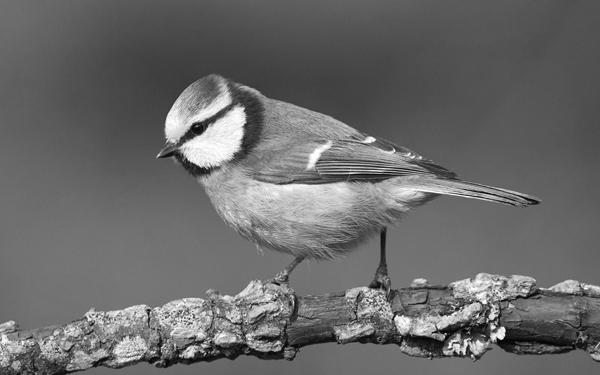
\includegraphics[width=\linewidth]{pics/bildverarbeitungsalgos/grayscaling_output.png}
    \caption{Input}
    \label{maai:thresholding:input:thrid}
  \end{minipage}
  \hfill
  \begin{minipage}[t]{0.45\linewidth}
    \centering
    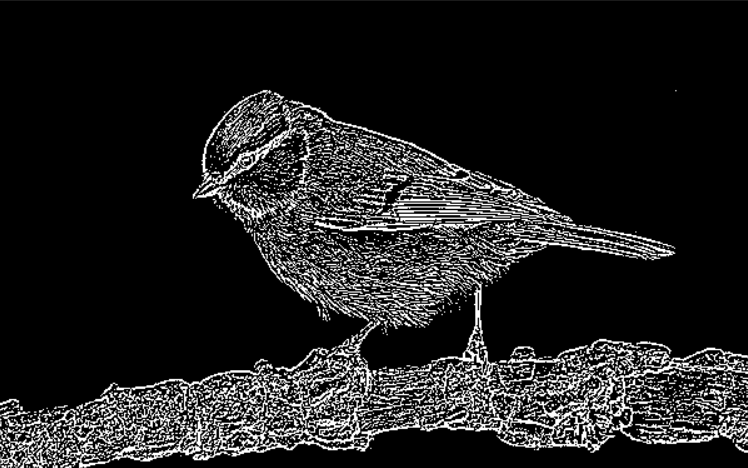
\includegraphics[width=\linewidth]{pics/bildverarbeitungsalgos/gaussian_thresholding.png}
    \caption{Output}
    \label{maai:gaussianthresholding:output}
  \end{minipage}
\end{figure}

\subsubsection{Detecting Contours}
Kantenerkennung ist wie die Graustufenkonvertierung (\ref{maai:grayscale}) oder das Weichzeichnen (\ref{maai:blurring}) ein Bildverarbeitungsalgorithmus, welcher dazu verwendet wird, um Diskontinuitäten zu identifizieren. Hierzu werden scharfe Änderungen der Bildfarbe/der Bildintensität herausgefiltert. Punkte, wo dieser Wert stark variiert, werden als Kante markiert.

Die Kantenerkennung schafft eine Basis für die Bildverarbeitung und Form Erkennung der Bild- und Objekterkennung. Für die Konturenerkennung sind jedoch nur geschlossene Kanten von Bedeutung.

Die Kantenerkennung funktioniert wie folgt. Für die ``Edge-Detection'' (Kantenerkennung) ist wie beim Weichzeichnungsalgorithmus (\ref{maai:blurring}) eine Konvolution nötig; vor allem, um hochauflösende Bilder zu verarbeiten. Oft wird dazu der sogenannte ``Sobel''-Operator herangezogen. Dieser erzeugt für die Kantenerkennung zwei Kernel, welche in x- und y-Richtung unterteilt sind. Der Kernel in x-Richtung sieht wie folgt aus:

\[
  \left[\begin{array}{rrr}
      -1 & 0 & 1 \\
      -2 & 0 & 2 \\
      -1 & 0 & 1 \\
    \end{array}\right]
\]


Hier sind negative Nummern links und positive Nummern rechts. Wegen der 0 (null) in der Mitte des Kernels wird nur geprüft, ob eine vertikale Linie/Kontur nach unten existiert. Daher wird mit diesem Kernel nur in x-Richtung auf eine Kante überprüft. Die mittigen Pixel auf der y-Achse des Kernels werden durch den ``Sobel''-Operator höher gewichtet als die Randpixel.

Das Ziel ist dabei einen Unterschied zwischen der Farb-/Lichtintensität des linksseitigen Bereichs des Bilds (der Pixel auf der linken Seite) und der Intensität des rechtsseitigen Bereichs des Bilds (der Pixel auf der rechten Seite) herauszufinden.

Anhand eines Beispiels wird diese Operation klarer:

\[
  \left[\begin{array}{rrrr}
      0 & 0 & 255 & 255 \\
      0 & 0 & 255 & 255 \\
      0 & 0 & 255 & 255 \\
      0 & 0 & 255 & 255 \\
    \end{array}\right]
\]

Hier existiert eine für einen Menschen klar erkennbare Kante; jedoch tut sich bei dem Erkennen die Maschine schwerer. Dazu muss der zuvor genannte Kernel über die Pixel gelegt werden. Das Ergebnis ist die Summe der Multiplikationen der einzelnen Werte des Kernels mit den entsprechenden Werten der Matrix des Bildes. Diese ergibt in diesem Beispiel 1025. Ist dieser Wert über einen zuvor definierten Schwellwert, so existiert an dieser Position eine Kante.

Für die Konturenerkennung wird ein Bereich von geschlossenen Kanten herangezogen. Diese geschlossenen Kanten werden erkannt, indem eine Kante in einem zuvor definierten Kernel rund um eine weitere Kante existiert. Führt dieser Pfad wieder zurück zur Ausgangskante, so kann mit Sicherheit gesagt werden, dass es sich um eine geschlossene Kontur handelt.

%Quelle:https://www.geeksforgeeks.org/find-and-draw-contours-using-opencv-python/


\begin{lstlisting}[caption=Adaptive Gaussian Thresholding,language=Python,label=maai:gaussianthresholding]
    
import cv2
import numpy as np

# Let's load a simple image with 3 black squares
image = cv2.imread(
    'path/to/image.png')
cv2.waitKey(0)

# Grayscale
gray = cv2.cvtColor(image, cv2.COLOR_BGR2GRAY)

# Find Canny edges
edged = cv2.Canny(gray, 30, 200)
cv2.waitKey(0)

# Finding Contours
# Use a copy of the image e.g. edged.copy()
# since findContours alters the image
contours, hierarchy = cv2.cv2.findContours(
    edged, cv2.RETR_LIST, cv2.CHAIN_APPROX_SIMPLE)

cv2.imshow('Canny Edges After Contouring', edged)
cv2.waitKey(0)

print("Number of Contours found = " + str(len(contours)))

# Draw all contours
# -1 signifies drawing all contours
cv2.drawContours(image, contours, -1, (255, 255, 0), 1)

cv2.imshow('Contours', image)
cv2.waitKey(0)
cv2.destroyAllWindows()

\end{lstlisting}

Dieser Programmcode erzeugt folgendes Bild:


\begin{figure}[htb]
  \centering
  \begin{minipage}[t]{0.45\linewidth}
    \centering
    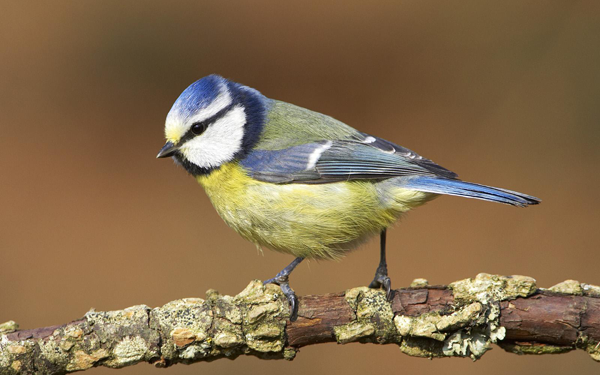
\includegraphics[width=\linewidth]{pics/bildverarbeitungsalgos/input.png}
    \caption{Input \cite{maai:input:cite}}
    \label{maai:getcounturs:input}
  \end{minipage}
  \hfill
  \begin{minipage}[t]{0.45\linewidth}
    \centering
    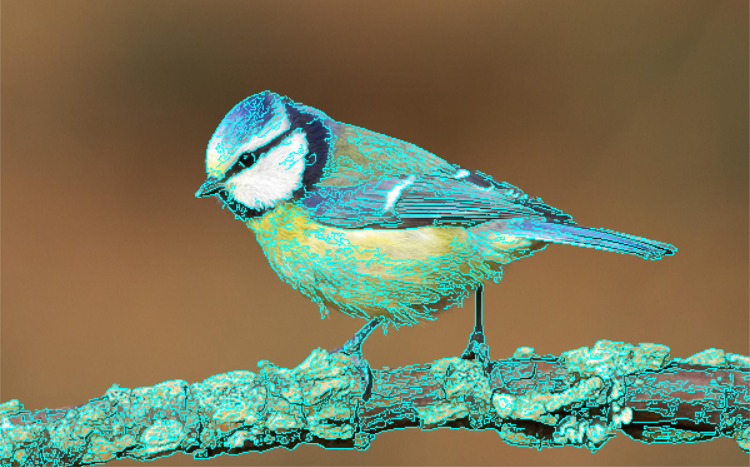
\includegraphics[width=\linewidth]{pics/bildverarbeitungsalgos/getcounturs_output.png}
    \caption{Output}
    \label{maai:getcounturs:output}
  \end{minipage}
\end{figure}

Die Quelle zu diesem Unterkapitel ist ein ``YouTube''-Video mit dem Titel ``Canny Edge Detector - Computerphile'' von dem Kanal ``Computerphile''. \cite{cannyedge:cite}

\subsubsection{ApproxPolyDP}\label{maai:approxpolydp:header}

Das Wissen zum folgenden Unterkapitel entspringt aus dem Blogpost von ``Devjyoti Chakraborty'' mit dem Namen ``OpenCV Contour Approximation''. \cite{approx:cite}
%Quelle: https://pyimagesearch.com/2021/10/06/opencv-contour-approximation/

Um nun aus den gewonnenen Konturen ein Blatt Papier zu erkennen, müssen die vier Eckpunkte des Blattes herausgefunden werden für eine Perspektiventransformation. Diese vier Punkte werden über die Open-Computer-Vision-Funktion ``approxPolyDp(\dots)'' (``approxymation of Polygon Points'' englisch für Annäherung von Polygonen) gewonnen. Die Funktion gibt aus einem übergebenen Konturen-Array (Array = Ansammlung an Daten; in diesem Fall eine Sammlung an Positionsdaten der Kontur-Eckpunkte), eine Annäherung der Eckpunkte zurück. In dem Feld werden die Punkte der Konturen als Vektoren angegeben. Die Annäherung an diese Punkte erfolgt mit einer übergebenen Genauigkeit, welche als Parameter der Funktion spezifiziert wird.

Diese Kontur Näherung, welche den ``Ramer–Douglas–Peucker'' Algorithmus (abgekürzt RDP.; Abbildung \ref{fig:map:rdpalgo}) verwendet, hat das Ziel eine Kontur, also eine Polygon-Line, zu vereinfachen. Dies passiert, indem der Algorithmus die Scheitelpunkte der Kontur bei einem gegebenen Schwellwert reduziert.


\begin{figure}[H]
  \centering
  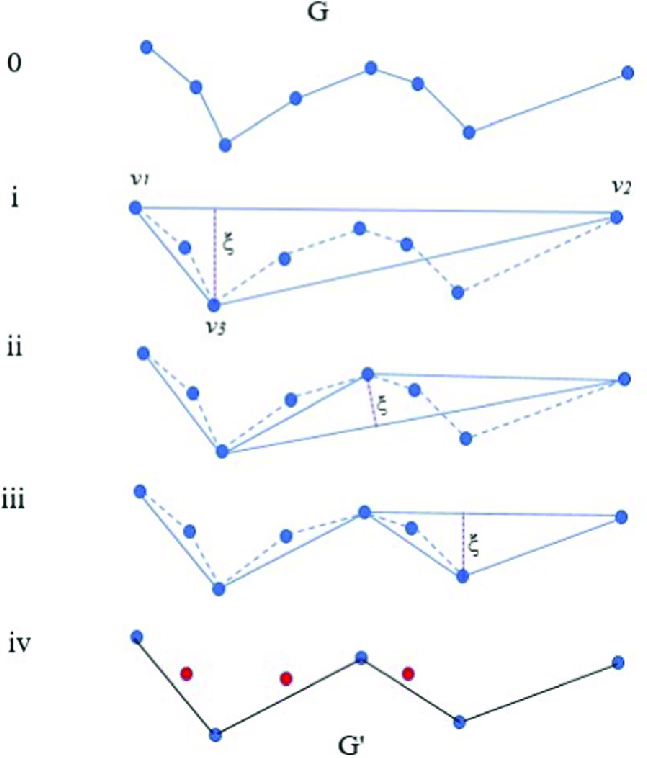
\includegraphics[scale=0.3]{pics/bildverarbeitungsalgos/The-Ramer-Douglas-Peucker-algorithm.png}
  \caption{Der Ramer–Douglas–Peucker Algorithmus \cite{maai:rdpa:cite}}
  \label{fig:map:rdpalgo}
\end{figure}
% Quelle: https://www.researchgate.net/figure/The-Ramer-Douglas-Peucker-algorithm_fig6_332499235

Wenn die Start- und Endpunkte einer Kurve gegeben sind, findet der Algorithmus zuerst den am weitest entfernten Punkt (Endpunkt). Dieser nimmt dann mit einem gegebenen Schwellwert \(x\) einen Bruchteil, welcher zu der Anzahl \(x\) an Polygonpunkten führt, der originalen Kontur her. Der gefragte Punkt, welcher sich an der Stelle des Bruchteils befindet, wird als neuer Konturpunkt herangezogen. Wenn andere Kontur-Punkte dazwischen liegen, so werden diese für den neuen, vereinfachten Konturen-Array ignoriert beziehungsweise eliminiert. Somit werden bestimmte Vertices (Eckpunkte) systematisch eliminiert.

Über bleibt eine Annäherung an eine Ausgangskurve. Somit bleibt am Ende genügend Information über, um zum Beispiel ein Blatt Papier erkennen zu können, was das Hauptziel von diesem Teil der Arbeit (Maperkennung) war. Dabei werden so viel Daten wie möglich aus den Konturen entfernt und die Verarbeitung kann schneller erfolgen.

Dieses Verfahren wird auch als Kurvenglättung bezeichnet.

Außerdem werden maximal vier Punkte für eine Perspektiventransformation herangezogen.

Das heißt, dass die Scheitelpunkte einer Kurve reduziert werden und dabei trotzdem eine große Menge beziehungsweise Genauigkeit an Information erhalten bleibt. Somit bleibt ein Großteil der Form beibehalten.

Somit werden die vier Eckpunkte des Blatt Papiers in dieser Arbeit herausgefunden. Diese vier Eckpunkte sind eine sehr genaue Annäherung an die Eckpunkte, so wie diese in der Realität vorzufinden sind.

Wie dies mit Python und OpenCV2 umgesetzt wurde, wird im folgenden Codebeispiel ersichtlich:


\begin{lstlisting}[language=Python,caption=ApproxPolyDP Beispiel,label=maai:approxpolydp:code]
    #importing the module cv2
    import cv2

    #reading the image whose shape is to be detected using imread() function
    imageread = cv2.imread('Path/to/image.png')

    #converting the input image to grayscale image using cvtColor() function
    imagegray = cv2.cvtColor(imageread, cv2.COLOR_BGR2GRAY)

    #using threshold() function to convert the grayscale image to binary image
    _, imagethreshold = cv2.threshold(imagegray, 245, 255, cv2.THRESH_BINARY_INV)

    #finding the contours in the given image using findContours() function
    imagecontours, _ = cv2.findContours(imagethreshold, cv2.RETR_TREE, cv2.CHAIN_APPROX_SIMPLE)

    #for each of the contours detected, the shape of the contours is approximated using approxPolyDP() function and the contours are drawn in the image using drawContours() function
    for count in imagecontours:
    epsilon = 0.01 * cv2.arcLength(count, True)
    approximations = cv2.approxPolyDP(count, epsilon, True)
    cv2.drawContours(imageread, [approximations], 0, (0), 3)
    
    #displaying the resulting image as the output on the screen
    cv2.imshow("Resulting_image", imageread)
    cv2.waitKey(0)
\end{lstlisting}
%Quelle: Zitat: https://www.educba.com/opencv-approxpolydp/

Dieser Programmcode führt zu folgendem Ergebnis:


\begin{figure}[htb]
  \centering
  \begin{minipage}[t]{0.45\linewidth}
    \centering
    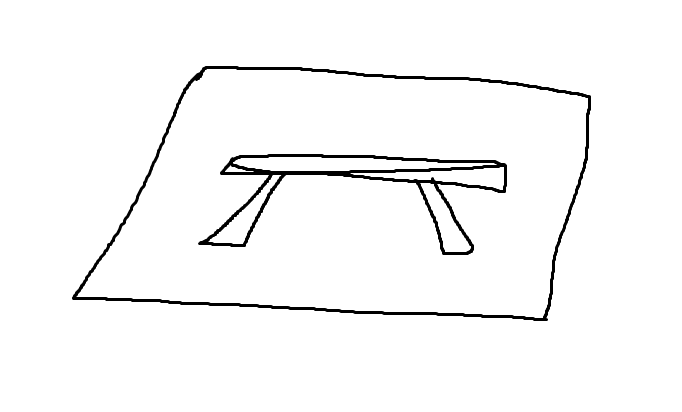
\includegraphics[width=\linewidth]{pics/bildverarbeitungsalgos/ApproxPolyDP_input.png}
    \caption{Input}
    \label{maai:approxpolydp:input}
  \end{minipage}
  \hfill
  \begin{minipage}[t]{0.45\linewidth}
    \centering
    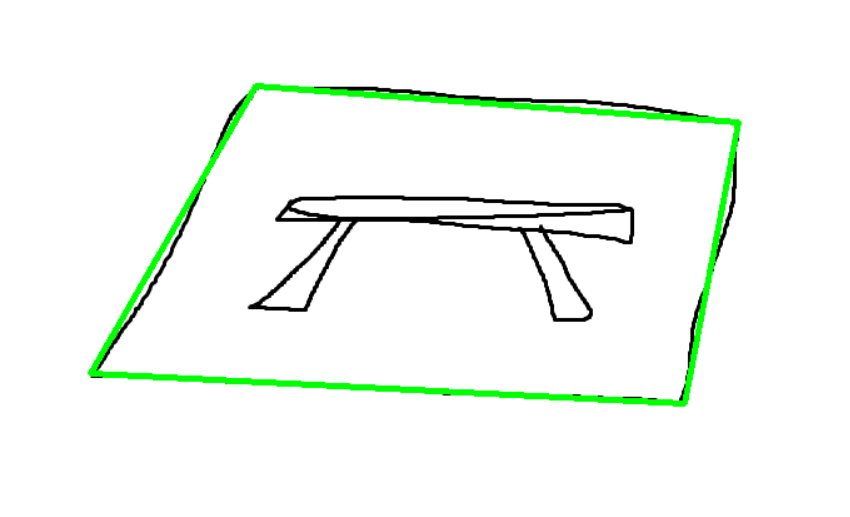
\includegraphics[width=\linewidth]{pics/bildverarbeitungsalgos/ApproxPolyDP_output.png}
    \caption{Erster Output des Programmcodes}
    \label{maai:approxpolydp:output}
  \end{minipage}
\end{figure}


\subsubsection{Warp Perspective}\label{maai:wrapPerspective}

``Warp Perspective'' ist Englisch und bedeutet ``Perspektiventransformation''. Der Bildverarbeitungsalgorithmus wird zur Perspektivenveränderung herangezogen. Dieser Algorithmus ist der letzte Schritt der Bildverarbeitung, welcher nötig ist, um das Blatt Papier, auf welchem eine Map gezeichnet ist, aus einem Bild zu erkennen.

Durch die Perspektiventransformation werden Winkel, Parallelität und Längen verändert, wodurch es zu einer Stauchung beziehungsweise Streckung eines Bildes kommt.

Der Algorithmus zur Transformation der Perspektive kann wie folgt beschrieben werden:
\[
  \left[\begin{array}{r}
      ti\_x' \\
      ti\_y' \\
      ti     \\
    \end{array}\right]
  = \left[\begin{array}{rrr}
      a_{ 1 } & a_{ 2 } & b_{ 1 } \\
      a_{ 3 } & a_{ 4 } & b_{ 2 } \\
      c_{ 1 } & c_{ 2 } & 1       \\
    \end{array}\right]
  * \left[\begin{array}{r}
      x \\
      y \\
      1 \\
    \end{array}\right]
\]
Auf der rechten Seite der Gleichung befindet sich die Transformationsmatrix als erster Faktor und der Input \(x\) und \(y\) als Vektor und 1 als zweiter Faktor.

Das Produkt daraus, also die linke Seite der Gleichung, gibt den Skalierungsfaktor an. Das heißt der Perspektiven-transformierte Punkte mit den Koordinaten \(x\) und \(y\) wird zu einem neuen Punkt \(P'\) mit den Koordinaten \(x'\) und \(y'\).

Die Transformationsmatrix ist eine Kombination aus folgenden Werten:
\[
  \left[\begin{array}{rr}
      a_{ 1 } & a_{ 2 } \\
      a_{ 3 } & a_{ 4 } \\
    \end{array}
    \right]
  \to
  \text{ Transformation hinsichtlich Rotation, Skalierung, etc. }
\]
\[
  \left[\begin{array}{r}
      b_{ 1 } \\
      b_{ 2 } \\
    \end{array}
    \right]
  \to
  \text{ Verschiebungsvektor }
\]
\[
  \left[\begin{array}{rr}
      c_{ 1 } & c_{ 2 } \\
    \end{array}
    \right]
  \to
  \text{ Projektionsvektor }
\]

Die acht Unbekannten in der Transformationsmatrix geben die Freiheitsgrade im Raum an.

Um die Matrix kalkulieren zu können müssen zuerst die vier Punkte der Eckpunktnäherung durch ``approxPolyDp'' herangezogen werden. Diese Funktion wurde im Kapitel \ref{maai:approxpolydp:header} erklärt. Die vier Eckpunkte, welche in die Vogelperspektive transformiert wurden, sollen ein neues Rechteck darstellen. Das heißt, dass die vier Punkte, welche zuvor im dreidimensionalen Raum die vier Ecken des Blatt Papiers darstellten, werden nun in ein Rechteck perspektiventransformiert. Dadurch wird das Bild in eine Perspektive, welche einen Blick von ``oben'' ermöglicht, umgewandelt, und richtig skaliert.

Somit werden acht Unbekannte und acht Gleichungen erzeugt, wodurch die Gleichungen in der Matrix-Form gelöst werden können. In OpenCV2 passiert diese Matrixkalkulation via der Funktion ``cv2. getPerspectiveTransform(points, points')''. Der erste Parameter stellt die Koordinaten im Ausgangsbild dar und der zweite stellt die Koordinaten im Ausgabebild dar.

Danach wird ``cv2.wrapPerspective(\dots)'' angewendet, um die Perspektive anhand der gegebenen Matrix zu verändern. Dafür wird aus dem Ausgangsbild ein Teil weggeschnitten und über bleibt der für das ``use-case'' (Anwendungsfall) interessante Teil. Es wird nur jenes Stück aus dem Bild verwendet, welches in den vier gewählten Eckpunkten liegt. Dieses wird in die Vogelperspektive umgewandelt.

Folgender Programmcode zeigt die Matrixrechnung anhand der Bibliothek OpenCV2 und der dazugehörigen Funktionen:



\begin{lstlisting}[language=Python,caption=Perspektiventransformation Beispiel,label=maai:approxpolydp:code]
    #importing the module cv2 and numpy
    import cv2
    import numpy as np

    #reading the image whose perspective is to be changed
    imageread = cv2.imread('C:/Users/admin/Desktop/plane.jpg')
    
    #specifying the points in the source image which is to be transformed to the corresponding points in the destination image
    points1 = np.float32([[0, 100], [700, 260], [0, 700], [700, 400]])
    points2 = np.float32([[0, 200], [600, 0], [0, 700], [1000, 700]])
    
    #applying getPerspectiveTransform() function to transform the perspective of the given source image to the corresponding points in the destination image
    resultimage = cv2.getPerspectiveTransform(points1, points2)
    
    #applying warpPerspective() function to fit the size of the resulting image from getPerspectiveTransform() function to the size of source image
    finalimage = cv2.warpPerspective(imageread, resultimage, (500, 600))
    
    #displaying the original image and the transformed image as the output on the screen
    cv2.imshow('Source_image', imageread)
    cv2.imshow('Destination_image', finalimage)
    cv2.waitKey(0)
    cv2.destroyAllWindows()
\end{lstlisting}
%Quelle: Zitat: https://www.educba.com/opencv-warpperspective/

Dieser Programmcode führt zu folgendem Ergebnis:


\begin{figure}[H]
  \centering
  \begin{minipage}[t]{0.45\linewidth}
    \centering
    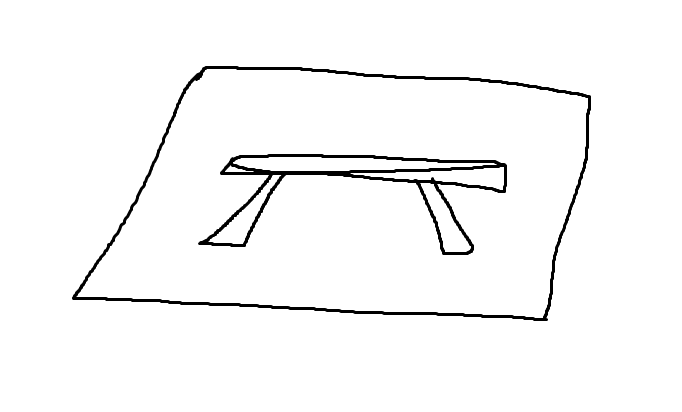
\includegraphics[width=\linewidth]{pics/bildverarbeitungsalgos/ApproxPolyDP_input.png}
    \caption{Input}
    \label{maai:wrapperspective:input}
  \end{minipage}
  \hfill
  \begin{minipage}[t]{0.45\linewidth}
    \centering
    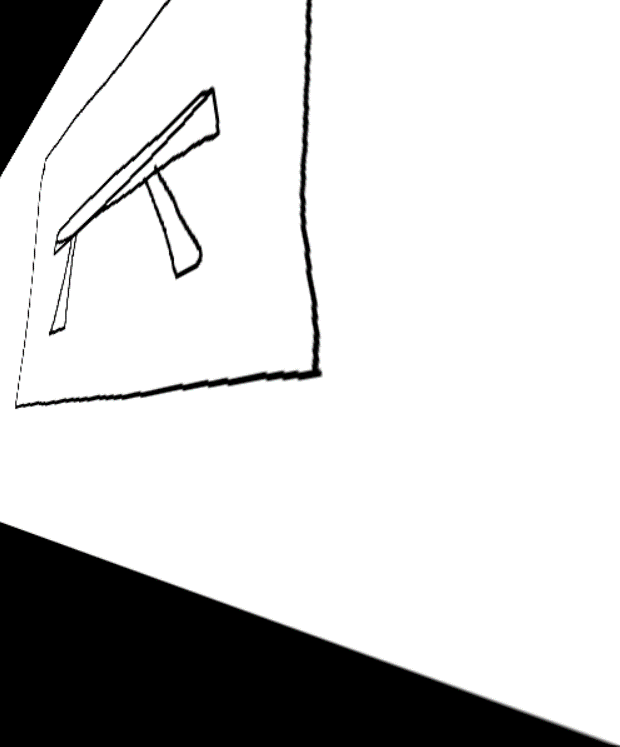
\includegraphics[width=\linewidth]{pics/bildverarbeitungsalgos/wrapperspective.png}
    \caption{perspektiventransformiert}
    \label{maai:wrapperspective:output}
  \end{minipage}
\end{figure}

Wissen zu diesem Unterkapitel wurde sich durch Erklärungen der Website ``educba.com'' angeeignet. \cite{educba}

\subsubsection{Umwandlung der Bilder in für das Spiel geeignete Daten [H]}\label{maai:udbifdsbd:head}
Ist die Perspektive des Bilds transformiert, so kann dieses mit dem ``Send-Button'' (Wie in Abbildung \ref{fig:map:maperkennungsprozess} ersichtlich) bestätigt werden.
Somit wird das Bild an den Python-Server ein letztes Mal zurückgesendet und es wird eine spielbare Map daraus generiert.
Wie dies Funktioniert wird in den folgenden Codeblöcken ersichtlich.

Zuerst wird sich darum gekümmert, dass die Daten so stark minimiert werden, dass sie trotzdem noch brauchbar sind, aber so viel wie möglich Informationen beinhalten. Das heißt: so wenig wie möglich Bildmaterial soll so viel wie möglich Information enthalten. Doch davor wird das übergebene Bild in den RGBA-Farbraum umgewandelt und in ein OpenCV2-Bild konvertiert. Im RGBA Farbraum ist es zusätzlich noch möglich neben den Farbwerten auch Informationen über die Transparenz des Bildes abzuspeichern. Dann startet wieder dasselbe Prozedere, wie bei der Perspektiven Transformation.

Zuerst wird das Bild in Graustufen konvertiert. Wie dies funktioniert ist bereits im Unterpunkt \ref{maai:grayscale} erklärt. Dann wird es unscharf gezeichnet und danach ein adaptiver Threshold (ein Schwellwert-Bild) daraus generiert.

Im nächsten Schritt wird die vorgefertigte Funktion ``Bitwise\_not'' angewendet. Hier wird das Bild in nur schwarze und weiße Pixel umgewandelt. Sie wandelt also alle Pixel entweder in schwarze oder weiße Bildpunkte um und generiert daraus wieder ein neues OpenCV2 Bild. Auch dieses Bild wird wieder unscharf gezeichnet.

Was dann noch für das Spiel wichtig ist, ist, dass das Bild in einen Quader umgewandelt wird. Das heißt, dass das Schwellwert-Bild so umgewandelt wird, dass alle Seiten (Höhe und Breite) gleich lang sind. Die leeren Flächen, die daraus entstehen werden mit transparenten Pixeln gefüllt.

Die Zeile zwanzig dient dazu das Bild testweise in einem Ordner abzuspeichern.

\begin{lstlisting}[language=Python,caption=Bild in Spielbare Map umwandeln,label=lst:umsetzung:getplayablearray]
    def getPlayableArray(img):
        np.set_printoptions(threshold=sys.maxsize)

        alpha_img = cv2.cvtColor(img, cv2.COLOR_BGR2BGRA)  # rgba
        imgWarpGray = cv2.cvtColor(alpha_img, cv2.COLOR_BGR2GRAY)
        blurred = cv2.GaussianBlur(imgWarpGray, (7, 7), 0)
        imgAdaptiveThre = cv2.adaptiveThreshold(
            blurred, 255, cv2.ADAPTIVE_THRESH_GAUSSIAN_C, cv2.THRESH_BINARY_INV, 7, 2)
        imgAdaptiveThre = cv2.bitwise_not(imgAdaptiveThre)
        imgAdaptiveThre = cv2.medianBlur(imgAdaptiveThre, 3)

        # make image square
        imgAdaptiveThre = np.array(makeSquare(
            cv2.cvtColor(imgAdaptiveThre, cv2.COLOR_BGR2BGRA)))

        img = cv2.cvtColor(imgAdaptiveThre, cv2.COLOR_BGR2BGRA)

        # pippoRGBA2 = Image.fromarray(np.array(img).astype('uint8'), mode='RGBA')
        # pippoRGBA2.show()
        cv2.imwrite('./source/prototypes/streamFusion/output/imgAdaptiveThre.png', imgAdaptiveThre)
\end{lstlisting}

Im nächsten Schritt wird der Array berechnet, welcher als Grundlage für die spielbare Map dient und aus dem aufgenommenen Bild extrahiert wird. Der Array beinhaltet nach der Verarbeitung schwarze und transparente Bildpunkte. Die schwarzen Pixel symbolisieren jene Plätze, auf welchen sich der Spieler schlussendlich bewegen kann. Die transparenten Pixel sind jene, welche als Hintergrund erkannt wurden und somit nicht für den Spieler begehbar sein sollten. Wie sich jedoch der Spieler auf diesen Punkten bewegen kann und wie der Array in die Spiellogik implementiert wird, wird im Kapitel ``Erstellung der Spielumgebung \ref{impl:Spielumgebung}'' von Rafetseder Tobias näher erklärt.

Jedoch wird zuerst das transformierte Bild in den Array umgewandelt. Dafür wird aus diesem adaptiven Threshold-Bild (Schwellwert-Bild) ein Faktor ausgerechnet, mit welchem die Bildpunkte zusammengefasst werden müssen, um insgesamt nicht mehr als \(\approx\)3025 Pixel zu überschreiten. Die dabei verwendete Formel wird im Folgenden an einem einfachen Beispiel erklärt. Diese lautet:

\[
  n \approx math.ceil(\sqrt{ \frac{ rows * columns }{ meshes } })
\]

Wird nun eine Bildbreite und eine Bildhöhe in ``rows'' und ``columns'' eingesetzt, so ist das Ergebnis der ganzzahlige Faktor, mit welchem die angegebene Bildbreite und Höhe multipliziert werden muss, um maximal \(\approx\)3025 Pixel zu erreichen.
Angenommen also, das Bild ist 1920x1080 Pixel groß, so würde das eine Anzahl von 2.073.600 Pixel liefern. Werden diese Werte in die Formel eingesetzt, so ist der Faktor 27. Wenn die beiden Bildmaße mit diesem Wert dividiert werden, so ist das Ergebnis ein Bild, welches 72x40 groß ist und somit eine Anzahl von 2880 Pixel liefert und somit weit unter den geforderten 3025 Pixeln liegt.

Der Grund, warum der Array eine maximale Größe von 3025 Einträgen hat, ist, weil p5.js, die Bibliothek, welche verwendet wurde, um die Spielumgebung aufzubauen nur ein Maximum von 1000 ``Meshes'' generieren kann, bevor das Spiel zu ``ruckeln'' beginnt. Es wird davon ausgegangen, dass nie mehr als ein Drittel seines Blattes vollgezeichnet wird.

Dann wird in einer zweidimensionalen Schleife das Bild durchgegangen und jeweils alle n Pixel ein Mittelwert errechnen über die Farbwerte des Bildes errechnet und somit der Hintergrund vom Vordergrund getrennt. Alle n Pixel werden zusammengefasst. Wenn in diesem Code also mehr als 95\% der Pixel Hintergrund darstellen, so wird der Pixel auch als Hintergrund gewertet (es wird also in den Map-Array ein transparenter Pixel an der Stelle x/n und y/n gepusht). Ansonsten wird ein schwarzer Pixel (als Map erkannt) dem Map-Array hinzugefügt. An dem Punkt mit den Koordinaten x/n und y/n befindet sich also der neue Bildpunkt, da das Bild komprimiert werden soll.

Dieser Map-Array wird in ein File abgespeichert. Dieses File dient rein dazu, um den Array debuggen zu können. Darunter wird ein Bild, welches aus diesem Map-Array generiert worden ist, im angegebenen Pfad gespeichert.

\begin{lstlisting}[language=Python,label=lst:umsetzung:getArray,firstnumber=21]
        iar = np.asarray(img).tolist()

        rows = len(iar)
        columns = len(iar[0])

        meshes = 3025
        # percent = perc(rows * columns)
        percent = 95
        n = math.ceil(np.sqrt(rows * columns / meshes))
        x = 0
        y = 0

        newImg = []

        while y < rows:
            newImg.append([])
            while x < columns:

                i = 0
                j = 0
                bg = 0
                while i < n:
                    while j < n:
                        if (y + j) < rows and (x + i) < columns:
                            if np.all(iar[y + j][x + i][:3] == [255, 255, 255], 0):
                                bg += 1
                        else:
                            bg += 1
                        j += 1
                    j = 0
                    i += 1

                bgPercent = bg / (n**2)
                if (bgPercent < (percent / 100)):
                    newImg[int(y / n)].append([0, 0, 0, 255])
                else:
                    newImg[int(y / n)].append([255, 255, 255, 0])

                x += n
            x = 0
            y += n

        iar = np.asarray(newImg).tolist()
        with open('./source/prototypes/streamFusion/output/mapArray.txt', 'w') as f:
            f.writelines(repr(iar))

        # pippoRGBA2 = Image.fromarray(np.array(newImg).astype('uint8'), mode='RGBA')
        # pippoRGBA2.show()
        cv2.imwrite(
            './source/prototypes/streamFusion/output/newImg.png', np.array(newImg))

        return newImg

\end{lstlisting}

\subsection{Kommunikation mit der Lobby via Flask und Flask SocketIO [W]} \label{PythonSocket}
\setauthor{Weinzierl Ben}

Sobald die User auf den QR-Code klicken, bzw. diesen scannen, werden sie zu der Map Erkennung weitergeleitet.
Dabei werden 2 Parameter mitgeschickt; Die Game-ID und die Client-ID. Damit der Python-Server diese Parameter entgegennehmen kann wird eine neue Route definiert. Danach werden die Pfadparameter abgespeichert,
und die HTML-Seite wird geladen (\ref*{PythonParam}). Daraufhin werden die Parameter im Localstorage gespeichert (\ref*{localstorage_map}). Dafür wird der Pfad der URL ausgelesen. Dieser wird aufgesplitet und dann im Localstorage abgespeichert.
\begin{figure}[H]
  \centering
  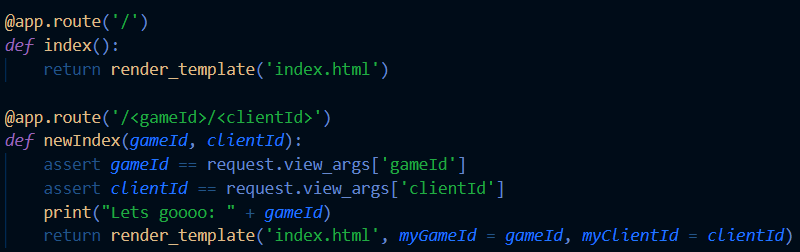
\includegraphics[scale=0.85]{pics/python_Params.png}
  \caption{Python Path Parameter}
  \label{PythonParam}
\end{figure}



\begin{figure}[H]
  \centering
  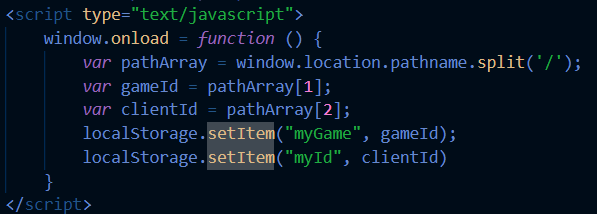
\includegraphics[scale=0.85]{pics/localStorage.png}
  \caption{Localstorage}
  \label{localstorage_map}
\end{figure}

Um nun die Multiuserfähigkeit zu gewährleisten wird nach jedem ``socket.on'' geprüft,
von welcher Game-ID und welchem Client der Request kommt. Dafür werden die gameId und clientId der msg mit der des Localstorages verglichen.

\begin{lstlisting}[language=Python,caption= Socket.on Beispielüberprüfung]
    socket.on('perspective transformed', function (msg) {
        let gameId = msg.gameId;
        let clientId = msg.clientId;
        let localGameId = localStorage.getItem("myGame");
        let localClientId = localStorage.getItem("myId")
        if (gameId != localGameId && clientId != localClientId) {
            console.log("Falscher Client/Game");
        } else {
            ...
        }
\end{lstlisting}

Sobald eine spielbare Map erstellt worden ist, wird eine SocketVerbindung zur Lobby hergestellt und dieser wird das Hintergrundbild und der mapstring geschickt.

\begin{lstlisting}[language=Python,caption=Map wird an Lobby geschickt]
    const lobbySocket = io('http://localhost:3001')
        const payLoad = {
            "method": "picUploaded",
            "clientId": clientId,
            "gameId": gameId,
            "img": img,
            "map": map
        }

    lobbySocket.emit('picUploaded', payLoad)
\end{lstlisting}

Wie es danach in der Lobby weitergeht wurde in \ref{SocketLobby} erläutert.

\section{KI [H]}\label{maai:ai:title}
\setauthor{Himmetsberger Jonas}
Die Vorstellung von Künstlichen Intelligenzen gibt es schon seit Mitte des zwanzigsten Jahrhunderts. Bei einer Konferenz von Wissenschaftlern am Dartmouth College im US-Bundesstaat New Hampshire im Jahr 1956 wird das erste Mal bewiesen, dass es möglich ist mit Mathematik menschliche Intelligenz zu simulieren. \cite{kigeschichte}

%Quelle: https://www.bosch.com/de/stories/geschichte-der-kuenstlichen-intelligenz/
Der Gedanke, dass eine von Menschenhand erschaffene Intelligenz, welche keine biologische Abstammung hat und den Menschen bei der Arbeit unterstützen, oder diese ganz abnehmen kann, wird seit diesem Ereignis angestrebt. Dabei ist das Feld, in welchem ``Artificial Intelligence'' (AI) beziehungsweise Künstliche Intelligenz (KI) eingesetzt werden kann, scheinbar unbegrenzt.

Das Einzige, das gegeben sein muss, ist, dass in einem komplexen System, in welcher die Künstliche Intelligenz operiert, Daten extrahiert und gesammelt werden können. Weiters sind Ressourcen, wie Hardware oder Zeit, ein wichtiger Aspekt. Die intelligente Maschine kann mehrere Millionen Schritte pro Tag ausführen und mit mehreren ``Gehirnen'' (mehrere Instanzen des Lernumfelds) gleichzeitig lernen. Trotzdem ist dies limitiert, durch die Geschwindigkeit und der Rechenleistung, die zu diesem Zeitpunkt aufgebracht werden kann, mit welcher die Aktionen ausgeführt werden und somit zu einem ``Lernen'' führen.

Die zuvor genannte Lerntechnik ``Reinforcement Learning'' (Kapitel \ref{tech:reinfLearning:header}), funktioniert ähnlich wie die Lern-Art von biologischen Organismen. Die Idee ist, dass simple, Lebensformen, welche nicht mehr als Instinkte zum Futter sammeln, Prädatoren ausweichen und im Generellen zum Überleben haben, sollten von einer Maschine ``leicht'' simuliert werden können. Ein Beispiel hierfür wäre ein Fadenwurm. Das ZNS (Zentrale Nervensystem) baut sich aus dreihundertzwei Nervenzellen zusammen. Weitere chemische Verbindungsstellen und Kanäle erhöhen die Komplexität dieses Lebewesens nur wenig. Dies ist mit modernen Computern bereits simulierbar. \cite{worm}
%Quelle: https://www.sueddeutsche.de/wissen/gehirngroesse-von-0-bis-11-000-000-000-neuronen-1.1850384

Dazu müssen jedoch gewisse mathematische Modelle angewandt werden, um dieses Ergebnis zu erreichen und den Organismus zu simulieren.

Dass und wie es für eine Maschine möglich ist zu lernen wurde bereits im Kapitel \ref{tech:ki:head} näher erläutert.

Um diese mathematischen Modelle jedoch perfekt auf ein gewünschtes Ergebnis abstimmen zu können, wird Hpyerparamter-``Fine-Tuning'' angewendet. Dabei werden jene Parameter, welche zu einem Lernen beitragen, so angepasst, dass das Modell eine perfekte Lernkurve erzielt.

Im Zuge dieser Arbeit wurde klar, dass Künstliche Intelligenz kein Thema ist, welches leicht zu begreifen ist.

Diese zuvor erwähnten mathematischen Modelle wurden bereits in einer Python Bibliothek namens ``Stable\_baselines3'' implementiert. Dieses Framework wird im Folgenden (Kapitel: \ref{maai:usedLibraries}) genauer erklärt.

Die zur Verfügung gestellten Algorithmen sind jedoch nicht perfekt auf unseren Anwendungsfall abgestimmt. Trotzdem wurden Ergebnisse erzielt (auch, wenn diese nicht bemerkenswert sind).

Die Logik der Welt, in welcher sich der Agent (Reinforcement-Learning) bewegt, wurde mittels Open-AI-Gym umgesetzt. Dabei handelt es sich um eine Hilfestellung, welche es ermöglicht objektorientiert eine Künstliche Intelligenz mit Python umzusetzen. Die Syntax beziehungsweise Vorgehensweise, welche verwendet wird, um eine Künstliche Intelligenz, welche mit der Methode des verstärkten Lernens trainiert, mittels Python zu implementieren, wird in den folgenden Kapiteln genauer beschrieben. Dabei wird auch genauer auf die genannten Bibliotheken eingegangen.

\subsection{Verwendete Bibliotheken [H]}\label{maai:usedLibraries}


Die Aufgabe von ``OpenAI-Gym'' ist, Reinforcement-Learning Algorithmen auf einem Beginner Niveau beizubringen und diese hauptsächlich zum Ausprobieren und Vergleichen zur Verfügung zu stellen.

Dabei stellt ``OpenAI-Gym'' viele vorab entwickelte Videospiele zur Verfügung. Diese Spiele sind hauptsächlich Atari-Games, wie zum Beispiel Tetris, Pac-Man, oder Breakout. Atari ist eine Spielkonsole aus den 1980' Jahren.

Diese Bibliothek stellt jedoch nicht nur zweidimensionale Umwelten zu Verfügung. Auch einige dreidimensionale Umgebungen, wie ``Humanoid'', bei welchem einer Figur das Gehen beigebracht werden muss, sind zur Auswahl.

Somit ist es für jeden möglich sich spielerisch mit dem Thema der Künstlichen Intelligenz auseinanderzusetzen. Es ist bereits mit einigen, wenigen Code-Zeilen möglich die ``Library'' einzubinden und ein simples Programm umzusetzen. \cite{ooaigymdocs}
\begin{lstlisting}[language=Python,label=lst:maap:simpleGym,caption=Simples OpenAI-Gym Programm]
    # import dependencies
    import gym 

    # create CartPole environment
    env = gym.make('CartPole-v0') 

    # reset the environment
    env.reset() 

    # walk 1000 steps
    for _ in range(1000): 
        # display progress visually
        env.render() 
        # take a random action
        env.step(env.action_space.sample()) 
        
    # close the environment after it is done
    env.close()
\end{lstlisting}


In diesem Environment (Spielumgebung) wird versucht einen Stab mithilfe einer beweglichen Plattform zu balancieren. Die Plattform kann sich dabei nur in einer Dimension (auf der X-Achse) bewegen. Mit diesem Beispielcode (\ref{lst:maap:simpleGym}) wird jedoch noch keine Künstliche Intelligenz trainiert. Hier werden zunächst zufällige Aktionen in dem Spiel ausgeführt, was selbstverständlich noch nicht zu einem gewünschten Ergebnis führt. Die Schwierigkeit dabei ist, dass sich die Plattform nicht nach links bewegt, wenn der Stab nach links fällt, oder umgekehrt, sondern den Stab wirklich balanciert. Diesen Ablauf der Bewegung findet der Algorithmus binnen weniger Sekunden heraus.

Es ist jedoch möglich dieses Programm so zu erweitern, dass dieses auch dazulernt.

Außerdem kann mit ``OpenAI-Gym'' ein eigenes Spiel erstellt werden \cite{ooaigymdocs}. Dies funktioniert objektorientiert. Dabei müssen folgende Funktionen eingebunden werden:

%Quelle: https://gym.openai.com/docs/

\begin{compactenum}
  \item \_\_init\_\_(self): diese Funktion wird aufgerufen, wenn ein Objekt der Klasse erstellt wird. Diese Methode wird auch ``Konstruktor'' genannt. Hier werden alle Parameter des Objekts initialisiert.
  \item step(self): Step(\dots) ist das Herzstück der Klasse. Hier wird jeder Schritt der Künstlichen Intelligenz definiert. Dazu wird zunächst eine Aktion definiert, welche die Maschine ausführen soll. Danach wird observiert, was sich in der Umgebung verändert hat und daraus ein Schluss gezogen, ob die Aktion zu einem guten, schlechten oder gar keinem Ergebnis führte; es wird also die Belohnung errechnet. Der Rückgabewert besteht dann aus den Observationen, der Belohnung, dem Status der Episode, welche die Künstliche Intelligenz zurzeit erlernt und einer beliebigen Zusatzinformation.
  \item render(self): Render(\dots) kann optional implementiert werden. Diese Funktion dient dazu dem Anwender den Lernfortschritt visuell darzustellen.
  \item reset(): die vierte und letzte Funktion ist Reset(\dots). Diese wird dazu verwendet um nach einer Episode die Umgebung und alle dazugehörigen Variablen auf einen gewünschten Stand zurückzusetzen. Als return Wert wird der aktuelle Stand der Künstlichen Intelligenz (die ``Observation'') zurückgegeben.
\end{compactenum}

Für die Beschreibung einzelner Begriffe empfiehlt es sich folgendes Kapitel zu lesen: ``Künstliche Intelligenz allgemein'' (\ref {tech:ki:head})

Die ScribbleFight-KI wurde wie folgt in Python implementiert:

Zunächst werden die Dependencies importiert.
\begin{lstlisting}[language=Python,label=lst:maap:scribblefightki,caption=ScribbleFight-KI OpenAI-Gym Environment]
    # Import dependencies
    import gym
    from gym.spaces import MultiDiscrete, Box
    from KI_v01.env.game import Game
\end{lstlisting}

Die Klasse CustomEnv, welche von ``gym.Env'' erbt wird wie folgt implementiert:

\begin{lstlisting}[language=Python,firstnumber=5]
    class CustomEnv(gym.Env):

        '''
        This class is a custom open-ai gym environment
        It has helper functions which are implemented below
        '''

        #metadata = {'render.modes' : ['human']}
        def __init__(self):
            # in the init function a new ScribbleFight instance is created
            self.pygame = Game()
            
            # the actionspace is defined by a MultiDiscrete set of random numbers
            '''DISCRETE[0]: ANGLE+, ANGLE-, idle
            DISCRETE[1]: "SPACE", "E", "Q", "R", "C", "F", "LEFTCLICK", idle
            DISCRETE[2]: "A", "D", idle'''
            self.action_space = MultiDiscrete([3, 8, 3])

            # the observationspace has the size of the visual copy Array (165x165), 
            # which is the vision of the AI
            '''random output when observation_space is sampled:
            [[0,0,0,...],
            [0,1,0,...],
                .....,
            [0,1,3,...],
            [0,1,5,...]]'''
            self.observation_space = Box(0, 10, (165, 165), int)

        def reset(self):
            # the reset function resets the game
            self.pygame.reset()
            obs = self.pygame.observe()
            return obs

        def step(self, actions):
            # in the step function a step is made
            self.pygame.action(actions)
            obs = self.pygame.observe()
            # checks if observations are valid
            #   if true then there are no observations made
            ''' 
            comparison = obs == Box(0, 0, (165, 165), int).sample()
            equal_arrays = comparison.all()
            print(equal_arrays)
            '''
            reward = self.pygame.evaluate()
            done = self.pygame.is_done()

            # info = self.pygame.info()  # not really needed
            return obs, reward, done, {}

        def render(self, mode="human", close=False):
            # this function renders the game
            self.pygame.view()

\end{lstlisting}


Eine weitere Bibliothek basierend auf Python, welche beim Erstellen der Reinforcement-Learning KI verwendet wurde, ist ``Stable-baselines-3''. Diese bietet auf eine zuverlässige Art und Weise die Implementierung von mathematischen Reinforcement-Learning Modellen. Dabei werden viele Algorithmen, wie zum Beispiel ``A2C'', ``DQN'', oder ``PPO'', zur Verfügung gestellt. Während dieser Arbeit wurden die Algorithmen ``A2C'' und ``PPO'' verglichen. In dem Fall der ``ScribbleFight'' KI, welche ziemlich komplex ist, hat die Recherche ergeben, dass diese zwei Arten, Modelle zu trainieren, am besten geeignet sind.

Eingebunden wird die Bibliothek wie folgt:
\begin{lstlisting}[language=Python,label=lst:maap:pposampleone,caption=Stable-Baselines3 Beispiel]
import gym

from stable_baselines3 import PPO
from stable_baselines3.common.env_util import make_vec_env

\end{lstlisting}

OpenAI-Gym kann verwendet werden, um ein Spielumgebung zu erschaffen. In diesem Beispiel wird wieder (wie in \ref{lst:maap:simpleGym}) die ``CartPole''-Welt verwendet. Damit die Effizienz des Lernens erhöht wird, kann durch das Erstellen der Umgebung mittels ``vec\_env'' eine Anzahl an Umgebungen gleichzeitig kreiert werden. Diese Anzahl wird als Parameter übergeben. Im folgenden Fall werden vier Umwelten gleichzeitig erstellt. All diese lernen auf dasselbe Modell. Dies wird auch ``Competitive Self-Play'' genannt. Danach wird dieses Environment an den PPO-Algorithmus übergeben. PPO steht für ``Proximal Policy Optimization''. Danach lernt die Maschine für 25.000 Schritte. Die Anzahl der Schritte haben nichts mit der Episodendauer zu tun. Ein Schritt ist entweder eine Bewegung nach links oder rechts. \cite{ppo}

%Quelle: https://openai.com/blog/openai-baselines-ppo/

\begin{lstlisting}[language=Python,firstnumber=6]

# Parallel environments
env = make_vec_env("CartPole-v1", n_envs=4)

model = PPO("MlpPolicy", env, verbose=1)
model.learn(total_timesteps=25000)
\end{lstlisting}

Nach dem Trainieren kann das Modell gespeichert und wiederverwendet werden. Dies passiert mittels ``PPO.load(\dots)''. Somit wird aus dem Gelernten ein Modell erstellt, welches verwendet werden kann, um vorhersagen zu treffen, darüber, wie sich die Plattform bewegen muss, um die Stange aufrecht zu erhalten.

\begin{lstlisting}[language=Python,firstnumber=12]

model.save("ppo_cartpole")

del model # remove to demonstrate saving and loading

model = PPO.load("ppo_cartpole")

obs = env.reset()
while True:
    action, _states = model.predict(obs)
    obs, rewards, dones, info = env.step(action)
    env.render()
\end{lstlisting}

Auf die Frage, wie die ``Reinforcement-Learning-Algorithmen'' funktionieren wird in dieser Arbeit nicht eingegangen.

% \subsection{Künstliche Intelligenz Definition [H]}

\subsection{Die ScribbleFight-KI [H]}\label{maai:scribblefightki}

Im Laufe der Ausarbeitung der Diplomarbeit und der damit zusammenhängenden Forschung änderte sich oft die
Vorstellung darüber, wie das Endprodukt (KI) auszusehen hat, beziehungsweise, wie dieses aussehen kann.
Limitierungen, welche vor der Forschung noch nicht bekannt und bewusst waren, begrenzten die Lernfähigkeit der KI.
Auf Probleme, Lösungen und Ergebnisse wird jedoch in diesem Kapitel noch näher eingegangen.

Die KI wurde auf einem ``Apple IMac 2017'' trainiert.

Das Ziel bestand darin eine Künstliche Intelligenz zu erschaffen, welche auf einem, für einen durchschnittlich guten, menschlichen Spieler, herausfordernden Niveau spielt. Dabei sollte diese:
\begin{compactitem}
  \item Alle möglichen Attacken erlernen,
  \item erlernen, in welchem Winkel ein Schuss abgefeuert werden muss, um einen Gegner zu treffen,
  \item lernen, wann eine Attacke, oder ein Schuss abgefeuert werden muss, um einen Gegner zu treffen,
  \item erlernen, wie ein Agent auf der Plattform bleibt, beziehungsweise was und wo diese ist,
  \item gegnerische Kugeln beziehungsweise Attacken erkennen und ausweichen.
\end{compactitem}
Im Laufe der Ausarbeitung der Künstlichen Intelligenz wurde jedoch klar, dass dies Ziele sind, welche im Zuge einer Diplomarbeit, in diesem Ausmaß, nicht erreichbar waren. %Die Künstliche Intelligenz lernte jedoch am schnellsten Wege die Plattform zu verlassen.

Damit die Maschine lernen kann, stellt das ScribbleFight-Frontend, welches mit Webtechnologien, wie HTML und JavaScript umgesetzt wurde, Informationen über den Spieler beziehungsweise Agenten zur Verfügung. Diese werden in einem ``myPlayer''-Objekt gespeichert. Das Objekt sieht wie folgt aus:

\begin{figure}[H]
  \centering
  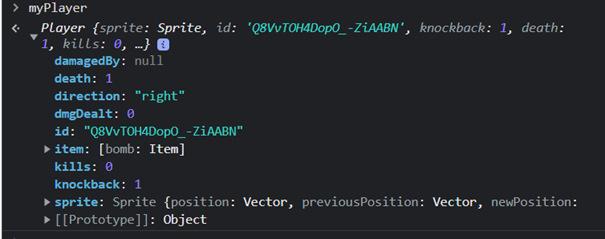
\includegraphics[scale=0.65]{pics/ai/myPlayer.png}
  \caption{``myPlayer''-Objekt}
  \label{fig:ai:myPlayerPic}
\end{figure}

Für die Künstliche Intelligenz sind Daten, wie ``death'' (Tode), ``dmgDealt'' (verteilten Schaden), ``kills'' (Anzahl an Spieler, welche von diesem Agenten von der Plattform gestoßen wurden) und ``knockback'' (Rückstoß, welcher der Spieler erleidet) von Bedeutung.
Damit die Werte des Objekts ausgelesen werden können wurde in Python folgende Funktion implementiert:

\begin{lstlisting}[language=Python,label=lst:maap:getstats,caption=Informationen über den Spieler]
def getStats(driver):
    dmgDealt, knockback, deaths, kills = 0, 0, 0, 0

    dmgDealt, knockback, deaths, kills = driver.execute_script(
        'return [myPlayer.dmgDealt, myPlayer.knockback, myPlayer.death, myPlayer.kills]')

    return dmgDealt, knockback, deaths, kills
\end{lstlisting}

Die Funktion extrahiert den für die KI relevanten Inhalt und gibt diese als return Wert wieder zurück. Dadurch wird die Maschine bei jedem Schritt über den Status des Spielers informiert.

% Ziele
% Umsetzung
% code (eher so vom rafi)
\subsubsection{Beschreibung der Funktionalität [H]}
Ein weiterer, zentraler Punkt der Ausarbeitung ist, wie die ``ScribbleFight''-KI zu sehen hat. Dies passiert mit einem zweidimensionalen Array, welcher ``visCopy'' im Frontend genannt wird. Die Einträge in diesem Feld sind die Zahlen von null bis zehn. Dieser wird erstellt, basierend auf den Inhalt des Spiels, welchen auch ein menschlicher Spieler sehen würde. Somit ist es für die KI nicht möglich, Daten zu manipulieren, auf welche ein Gegenspieler keinen Zugriff hätte. Dabei wird das Sichtfeld wie folgt codiert:
\begin{compactitem}\label{mappedPixels}
  \item 0: Hintergrund
  \item 1: Plattform
  \item 2: eigener Agent
  \item 3: Gegner
  \item 4: eigenes Projektil
  \item 5: gegnerisches Projektil
  \item 6: Bombe
  \item 7: Schwarzes Loch
  \item 8: Verkleinerung
  \item 9: Miene
  \item 10: Piano
\end{compactitem}

\begin{figure}[H]
  \centering
  \begin{minipage}[t]{0.45\linewidth}
    \centering
    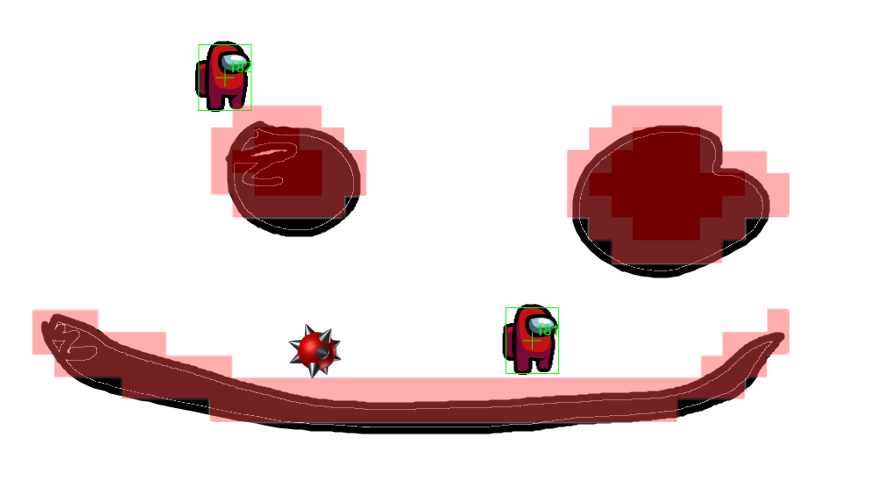
\includegraphics[width=\linewidth]{pics/ai/newView.png}
    \caption{Spieler Sicht}
    \label{maai:ai:newView}
  \end{minipage}
  \hfill
  \begin{minipage}[t]{0.45\linewidth}
    \centering
    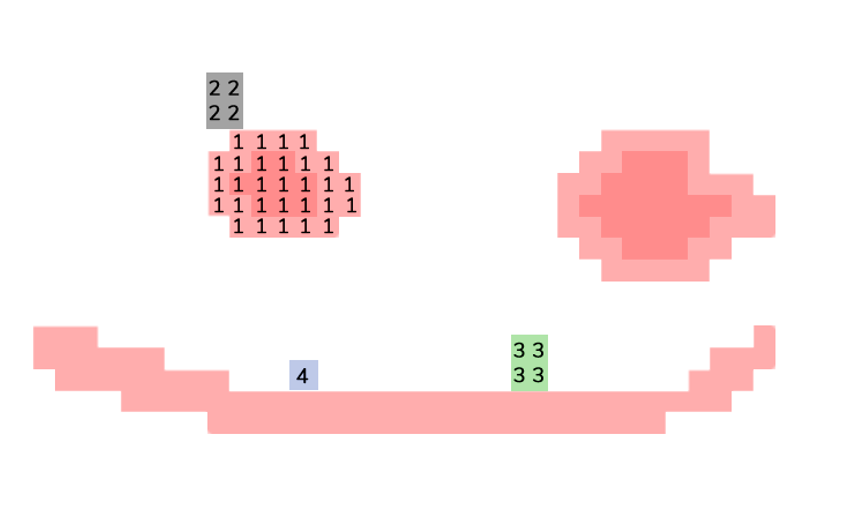
\includegraphics[width=\linewidth]{pics/ai/KIView.png}
    \caption{KI Sicht}
    \label{maai:ai:KIView}
  \end{minipage}
\end{figure}

Der ``Pixelclump'' ist ein zweidimensionaler Array von Pixelwerten (schwarz oder transparent, weiß) und wird von der Map-Erkennung (\ref{maai:maperkennung:head}) als Output zurückgeliefert. Dieses zweidimensionale Feld dient als Basis für den Untergrund, auf welchem sich die Spieler bewegen können. Um das Spiel in eine, für die Künstliche Intelligenz sichtbare Welt umzuwandeln, wird zunächst der ``Pixelclump'', um das Dreifache vergrößert. Gleichzeitig werden die Pixelwerte durch die oben angeführten Zahlen (von null bis zehn; Bedeutung: \ref{mappedPixels}) ausgetauscht. Durch die dreifache Skalierung der Spielumgebung von 55x55 auf 165x165 Werten, ist es möglich, dass die Künstliche Intelligenz dreimal genauer sieht, als ein Bildpunkt der Map aufgetragen wird. Somit kann genauer agiert werden und Spieler und Attacken besser erkannt werden (in der Theorie).

Die Aufskalierung und Umwandlung des Map-Arrays in den ``Visual''-Array passiert in der Funktion ``getVisualMap(\dots)'':
\begin{lstlisting}[language=Python,label=lst:maap:getVisualMap,caption=Umwandlung des Pixel-Clumps in eine für die KI sichtbare Darstellung]
/**
 * Converts standard map, which is 55x55 
 * into visual map which is 165x165 for better accuracy
 * 
 * @param {given arry which represents map} paramarr 
 * @returns new visual array
 */
function getVisualMap(paramarr) {
  let visual = []
  let factor = 3
  for (let i = 0; i < paramarr.length * factor; i++) {
    visual.push([])
    for (let j = 0; j < paramarr.length * factor; j++) {
      if (paramarr[int(i / factor)][int(j / factor)][3] > 0) {
        visual[i].push(1)
      } else {
        visual[i].push(0)
      }
    }
  }
  return visual
}
\end{lstlisting}
Mit jeder Bewegung und Aktualisierung von Status wird der ``visual''-Array in einen ``visCopy''-Array eingetragen. Dabei werden alle Entitäten neu hinzugefügt. Das Feld wird jedoch durch die Kopie nur an den Positionen verändert, wo auch eine Änderung passiert ist. Dadurch wird dieses nicht immer neu erstellt, und die Effizienz wird gesteigert. Außerdem, dadurch, dass Javascript zur kalkulation komplexer Berechnungen mehrere Threads zur Verfügung hat, kann das Verarbeiten dieses Arrays in einer Zeit passieren, welche die Bilder pro Sekunde des Spiels nicht verringert und somit für den Spieler nicht bemerkbar ist.
Der Codeblock \ref{lst:maap:addspritetovisual} beschreibt die Funktion mit welcher ein
Spielelement (``Sprite'') zu der KI-Sicht hinzugefügt wird.

\begin{lstlisting}[label=lst:maap:addspritetovisual,caption=Sprite in ``visCopy''-Array eintragen]
    function addSpriteToVisual(sprite, num) {
      if (visual != undefined && visCopy != undefined) {
        ...convert x and y coordinates of sprite in game into position in visCopy array
    
        for (let i = visualUnitX; i < maxXIterations; i++) {
          for (let j = visualUnitY; j < maxYIterations; j++) {
            // make sure to never overlay attacks with myPlayer or enemy
            // top priority has myPlayer
            if ((visCopy[j][i] != 2
              && visCopy[j][i] != 3)
              || num == 2)
              visCopy[j][i] = num;
          }
        }
      }
    }
\end{lstlisting}

Wird nun die bearbeitete Kopie des ``visual''-Arrays ausgeben, so ist der Output die Sicht der ``ScribbleFight'' Künstlichen Intelligenz. In der folgenden Abbildung wurden die Ziffern von null bis zehn in Farben umgewandelt. Das Bild \ref{maai:ai:visCopy:input} ist die Sicht des Spielers und das Bild \ref{maai:ai:visCopy:output} ist die Sicht der KI.

\begin{figure}[H]
  \centering
  \begin{minipage}[t]{0.45\linewidth}
    \centering
    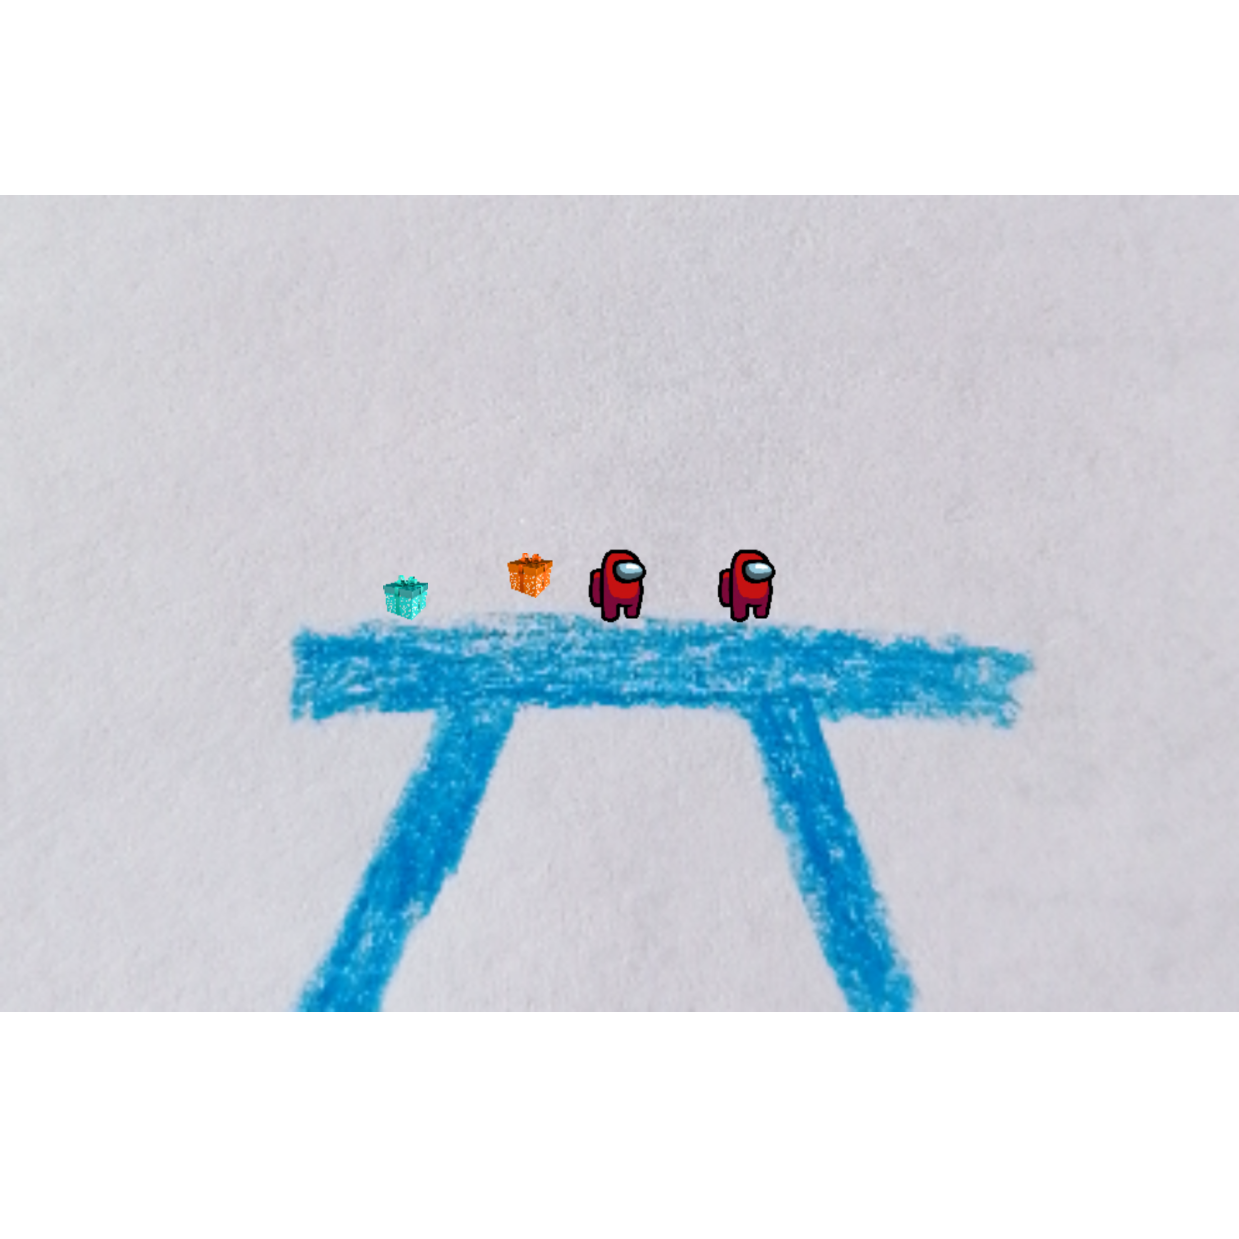
\includegraphics[width=\linewidth]{pics/ai/screenshots.png}
    \caption{Spieler Sicht}
    \label{maai:ai:visCopy:input}
  \end{minipage}
  \hfill
  \begin{minipage}[t]{0.45\linewidth}
    \centering
    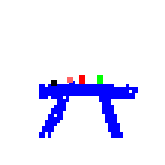
\includegraphics[width=\linewidth]{pics/ai/newImg.png}
    \caption{KI Sicht}
    \label{maai:ai:visCopy:output}
  \end{minipage}
\end{figure}

\subsection{ScribbleFight Reinforcement Learning Implementierung [H]}
Wie bereits in dem Kapitel ``Reinforcement Learning'' (\ref{tech:fig:reinfconcept}) erklärt, basiert diese Art des Lernens auf unpräparierte Daten. Das heißt, dass kein Trainingsset an Daten existiert, welches zum Lernen und Vergleichen verwendet wird, sondern ein Agent in eine ihm unbenannte Umwelt gesetzt wird und rein über ausprobieren lernt. Das einzige Ziel besteht darin, dass eine maximale Höhe an Belohnungen erreicht werden soll.

Im folgenden wird der Programmcode (\ref{lst:maai:game}), welcher diese Forderungen umsetzt, beschrieben.

Bevor die KI implementiert werden kann, muss eine Referenz auf das Browserspiel erzeugt werden. Dies passiert mit der Bibliothek namens ``Selenium''. Selenium ermöglicht es mit einem Python-Code ein Browser-Fenster zu öffnen, in welchem diverse Keyboard-Events und vieles mehr ausgeführt werden können. Dafür werdeh zunächst die Optionen, welche beim Öffnen ein Browserfenster berücksichtig werden, erstellt. Die Optionen besagen zum Beispiel, dass sich das Fenster an die Bildschirmgröße mit ``start-maximized'' anpasst. Die ``Url'' auf welche navigiert werden soll ist `` http://localhost:3000'', da hier das Spiel auf einem Node-Server, als lokale Instanz auf das Spiel, zur Verfügung gestellt wird.

\begin{lstlisting}[language=Python,label=lst:maai:game,caption=Implementation der Logik der Reinforcement Learning KI]
'''DEPENDENCIES'''
# selenium webdriver
from webdriver_manager.chrome import ChromeDriverManager
from selenium import webdriver

# options
from KI_v01.env.options.actions import *
from KI_v01.env.options.observations import *

# openai gym
from gym.spaces import Box


'''VARIABLES'''
FPS = 10

# selenium webdriver options
options = webdriver.ChromeOptions()
options.add_argument("start-maximized")
options.add_argument("disable-infobars")
port = 3000
url = 'http://localhost:%s' % (port)

\end{lstlisting}

Im folgenden Programmcode wird eine Klasse namens ``ScribbleFight'' erstellt.

In der \_\_init\_\_ Funktion, also dem Konstruktor der Klasse ``ScribbleFight'' werden alle Variablen und Konstanten initiiert und somit auf einen Startwert gesetzt. Dabei werden alle, für das Spiel relevanten Parameter auf einen ``Null-Wert'' gesetzt, da noch keine Daten gewonnen wurden. Auch Wahrheitsoperatoren, wie der ``readystate'', also ob das Browserfenster gestartet wurde oder nicht, werden hier gesetzt. Nach dem Erstellen wird das Fenster und somit das Spiel gestartet.

\begin{lstlisting}[language=Python,firstnumber=25]
class ScribbleFight:

    '''SCRIBBLE FIGHT GAME'''

    def __init__(self):
        self.driver = None
        self.playerId = 0
        self.obs = Box(0, 0, (165, 165), int).sample()
        self.dmgDealt = 0
        self.knockback = 0
        self.kills = 0
        self.deaths = 0
        self.just_died = False
        self.readystate = False
        self.startBrowser()
\end{lstlisting}

In der Funktion ``startBrowser'' wird ein neuer webdriver erstellt, über welchem später die Künstliche Intelligenz das Spiel steuert.
In einer Schleife wird überprüft, ob das Fenster bereits geöffnet wurde.

\begin{lstlisting}[language=Python,firstnumber=41]
    def startBrowser(self):
        self.driver = webdriver.Chrome(options=options,
                                       executable_path=ChromeDriverManager().install())
        self.driver.get(url)

        while not self.readystate:
            self.readystate = self.isReady()

    def isReady(self):
        try:
            self.playerId = self.driver.execute_script('return myPlayer.id;')
            return True
        except:
            return False
\end{lstlisting}

Die folgenden drei Funktionen sind ``update'', ``move'' und ``action''.

Update verwendet die zuvor erklärte ``getStats'' Methode (Code-Block \ref{lst:maap:getstats}) um den aktuellen Stand des Spielers wiederherzustellen, beziehungsweise die Informationen und den Status des Spielers zu aktualisieren.

Die Funktion ``action'' führt, basierend auf einem Übergabewert, eine Aktion aus. Diese Aktion kann eine Zahl zwischen null und sieben sein. Null stellt dabei zum Beispiel die Handlung ``jump'', also Springen, dar. Diese wird als ``Aktionsstring'' zurückübergeben.

In der Methode ``move'' wird ebenfalls ein Aktionsstring generiert. Jedoch wird hier eine links oder rechts Bewegung angestrebt, basierend auf Ziffern zwischen null und zwei. Die Aktion null steht für einen Schritt nach links, eins steht für einen Schritt nach rechts und zwei für ``keine Bewegung''.


\begin{lstlisting}[language=Python,firstnumber=56]
    def update(self):
        # get stats
        self.dmgDealt, self.knockback, self.deaths, self.kills = getStats(self.driver)

    def action(self, action, angle):
        # down ('s') action not implemented
        actionString = ''
        if action == 0:
            actionString = 'jump()'
        ...
        if action == 7:
            # idle state
            pass
        return actionString

    def move(self, action):
        actionString = ''
        if action == 0:
            actionString = 'moveLeft(); mirrorSpriteLeft();'
        if action == 2:
            # idle state
            pass
        return actionString
\end{lstlisting}


``observe'' ist dafür da, Observationen aus dem Spiel zu extrahieren.

In der Methode wird die Funktion ``readFromClient'' aufgerufen, welche den ``visCopy''-Array aus dem Frontend zurückgibt. Wie dieser Array funktioniert, was dieser ist und wie er erzeugt wird, wird im Kapitel ``Beschreibung der Funktionalität'' \ref{maai:beschrFunktionalitaet} erklärt.

Weiters wird überprüft, ob das Feld existiert. Sollte ``readFromClient'' ``false'' als Rückgabewert liefern, so wird ein neuer Array in derselben Dimension (zweidimensional) und Größenordnung (165x165) erstellt; jedoch mit lauter Nullen, welche für ein leeres Feld stehen. Liefert ``readFromClient'' ``visCopy'' als Rückgabewert zurück, so wird die Variable ``obs'' (Observation) mit diesem belegt.



\begin{lstlisting}[language=Python,firstnumber=78]
    def observe(self):
        visCopy = readFromClient(self.driver, 'return visCopy;')
        if visCopy:
            self.obs = visCopy
        if not visCopy:
            self.obs = Box(0, 0, (165, 165), int).sample()
    ...
\end{lstlisting}

Wie auch in der Klasse ``ScribbleFight'' (\ref{lst:maai:game}) beinhaltet ``Game'' zunächst eine ``\_\_init\_\_''-Funktion, welche als Konstruktor dient. Dieser setzt Startwerte der Parameter der Funktion. Beispielsweise wird als erstes eine Instanz auf ein Objekt der Klasse ``ScribbleFight'' erstellt. Variablen, welche ``previous\_'' als Präfix haben, dienen dazu den Unterschied zu einem vorherigen Schritt beziehungsweise Status herauszufinden. Die Implementation wird genauer in folgenden Codeblöcken beschrieben.


\begin{lstlisting}[language=Python,firstnumber=85]

class Game:

    '''AI INTERFACE TO SCRIBBLEFIGHT GAME INSTANCE'''

    def __init__(self):
        self.scribble_fight = ScribbleFight()
        self.min_game_length = 30 * FPS  # 1 min
        self.nothingChanged = 0  # player didn't accomplish anything in this timespan
        self.just_won = False  # the winning condition has yet to be implemented
        self.previous_damage_dealt = 0
        self.previous_knockback = 0
        self.previous_kills = 0
        self.previous_deaths = 0
        self.angle = 0  # angle in which the ai can shoot a bullet

\end{lstlisting}
In der ``action''-Funktion wird zunächst überprüft, ob das Spiel läuft. Danach wird ein ``String'' (Zeichenkette) namens ``actionString'' angelegt. Dieser wird leer initialisiert. Darunter wird der ``actionString'' basierend auf einem eindimensionalen Array, welcher drei Einträge hat, befüllt. Der erste Eintrag beinhaltet die Information, über die Richtung, in welche das Programm den Agenten beziehungsweise Spieler steuern möchte. Der nächste Eintrag bestimmt, welche Attacke die Künstliche Intelligenz ausführen möchte. An der letzten Position des Arrays wird bestimmt, wie die Künstliche Intelligenz den Abschusswinkel, in welchem sie das Projektil abfeuern möchte, anpassen soll. Ist dieser Wert des Arrays null, so wird der Winkel um fünf Grad gegen den Uhrzeigersinn angepasst. Umgekehrt passiert dies bei dem Wert eins. Zwei bewirkt, dass der Winkel gleichbleibt. Nachdem in der Funktion der ``actionString'' erstellt wird, wird dieser an die Methode ``execAction'' der ``ScribbleFight''-Instanz weitergegeben. ``execAction'' bewirkt die Ausführung der angegebenen Handlungen. Im Anschluss wird der Status des ``ScribbleFight'' Objekts und dessen Parameter aktualisiert.
\begin{lstlisting}[language=Python,firstnumber=101]
    def action(self, actions):
        # if current browser window has wrong url
        #   then dont execute actions
        if (self.scribble_fight.isPlaying() is False):
            return

        # take set of actions
        '''DISCRETE[0]: "A", "D", idle
        DISCRETE[1]: "SPACE", "E", "Q", "R", "C", "F", "LEFTCLICK", idle     
        DISCRETE[2]: ANGLE+, ANGLE-, idle'''
        actionString = ''

        actionString += self.scribble_fight.move(actions[0])
        actionString += self.scribble_fight.action(actions[1], self.angle)
        if actions[2] == 0:
            self.angle += 5
            if self.angle > 360:
                self.angle -= 360
        if actions[2] == 1:
            self.angle -= 5
            if self.angle < 0:
                self.angle += 360
        if actions[2] == 2:
            # idle state
            pass

        if actionString:
            self.scribble_fight.execAction(actionString)

        # update and save in-game stats
        self.scribble_fight.update()

\end{lstlisting}

Nachdem die vordefinierte Handlung der KI ausgeführt wurde, ist beim verstärkten Lernen der nächste Schritt, die Umwelt zu observieren. Der wohl wichtigste Schritt passiert danach. In der Funktion ``evaluate'' wird der Reward beziehungsweise die Belohnung berechnet. Dieser wurde wie folgt vergeben:
\begin{compactitem}
  \item hat der Agent der Künstlichen Intelligenz Schaden ausgeteilt (einem gegnerischem Spieler Schaden hinzugefügt), so wird der Belohnung eins addiert.
  \item erleidet der Agent Schaden, so wird der Belohnung eins subtrahiert.
  \item hat der Agent einen Spieler von der Plattform gestoßen beziehungsweise diesem so viel Schaden zugefügt, dass er stirbt, so wird als Belohnung eintausend Punkte vergeben.
  \item stirbt der Agent selbst, so wird eine negative Belohnung von 990 vergeben. Der Unterschied von zehn Punkten in der Entlohnung zwischen ``Gegner töten'' und ``selbst sterben'', wurde in der Hoffnung festgelegt, dass sich der Agent für einen ``Kill'' opfert.
\end{compactitem}


Nach der Evaluation der Belohnung wird überprüft, ob sich im Spiel etwas geändert hat. Wenn der Agent keinen ``Reward'' (null) erzielt hat, was bedeutet, dass er weder Schaden zugefügt, noch erlitten hat, keinen von der Plattform gestoßen hat und nicht selbst gestorben ist, so wird der Wert der Variable ``nothingChanged'' um eins erhöht.

Erreicht diese Variable eine gewisse Zahl erreicht hat, welche zuvor als Episodendauer definiert wurde (``min\_game\_length''), so wird in der Funktion der Wahrheitswert ``true'' (wahr) zurückgegeben, was so viel bedeutet, wie dass eine Episode beendet wurde. Die Variable ``min\_game\_length'' wurde als 30 * der Bilder pro Sekunde definiert. Dadurch wird eine Episode, in welcher sich für 30 Sekunden nichts ändert, abgebrochen. Eine Episode ist auch vorbei, wenn der Agent gewonnen hat, oder gestorben ist.
\newpage
Im folgenden Flussdiagramm wird dies etwas verständlicher erklärt.

\begin{figure}[H]
  \centering
  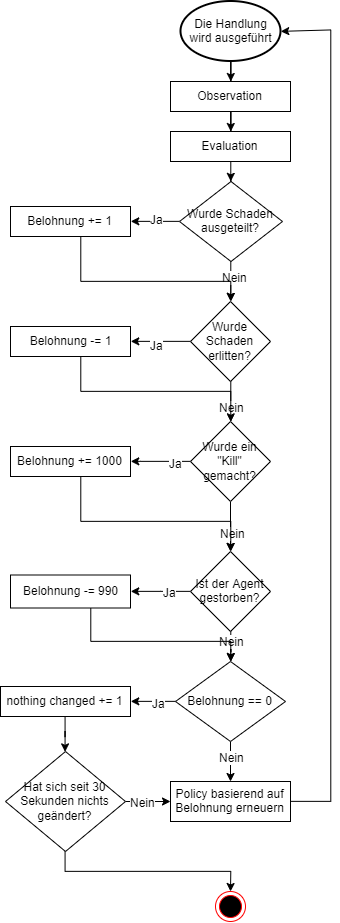
\includegraphics[scale=0.73]{pics/ai/Fluss.png}
  \caption{Ablauf des Lernens}
  \label{fig:maai:fluss}
\end{figure}


\begin{lstlisting}[language=Python,firstnumber=138]
    def observe(self):
        # get computer vision
        self.scribble_fight.observe()
        return self.scribble_fight.obs
        # return None

    def evaluate(self):
        reward = 0
        dmgDealt = self.scribble_fight.dmgDealt
        knockback = self.scribble_fight.knockback
        kills = self.scribble_fight.kills
        deaths = self.scribble_fight.deaths

        # evaluate reward
        # if reward is calculated then update previous_x varibales
        #   since they will be used for future comparison and reward calculation
        if dmgDealt > self.previous_damage_dealt:
            reward += 1
        if knockback > self.previous_knockback:
            reward -= 1
        if kills > self.previous_kills:
            reward += 1000
        if deaths > self.previous_deaths:
            # the reason why less reward is given when dying is because
            # I want the ai to be a killer machine
            reward -= 990
            self.scribble_fight.just_died = True

        self.previous_damage_dealt = dmgDealt
        self.previous_knockback = knockback
        self.previous_kills = kills
        self.previous_deaths = deaths

        if reward == 0:
            self.nothingChanged += 1
        else:
            self.nothingChanged = 0

        return reward

    def is_done(self):
        # returns if game won or nothing changed or agent died
        return self.scribble_fight.just_died or self.just_won or self.nothingChanged == self.min_game_length

\end{lstlisting}

In der Funktion ``reset'' werden die Variablen der Klasse ``Game'' zurückgesetzt.

``info'' alle gesammelten Informationen über den Spieler zurück. Diese Funktion wird allerdings nicht verwendet und wurde nur zur Vollständigkeit implementiert.

``view'' ist eine Methode, welche OpenAI-Gym abverlangt. In dieser das Spiel für den Programmierer der Künstlichen Intelligenz visuell angezeigt. Da jedoch ``ScribbleFight'' ein Frontend besitzt ist die Implementierung dieser Funktion sinnbefreit.


\begin{lstlisting}[language=Python,firstnumber=182]
    def reset(self):
        # reset position and observation
        if not self.scribble_fight.just_died:
            self.scribble_fight.resetPlayer()
        # reset in-game varibales
        self.scribble_fight.update()
        # reset variables
        # they should always be 0 because a reset only accures after death or as initialisation
        self.previous_damage_dealt = self.scribble_fight.dmgDealt  # should always be 0
        self.previous_knockback = self.scribble_fight.knockback  # should always be 1
        self.previous_kills = self.scribble_fight.kills  # should always be 0
        self.previous_deaths = self.scribble_fight.deaths
        self.nothingChanged = 0
        self.angle = 0

    def info(self):
        # return all infos about player
        #   not really needed tho
        return self.scribble_fight.dmgDealt, self.scribble_fight.knockback, self.scribble_fight.kills, self.scribble_fight.deaths

    def view(self):
        pass

\end{lstlisting}

\subsection{Evaluation der ScribbleFight KI [H]}

Im Laufe der Arbeit war der Teil ``ScribbleFight KI'' stark mit Forschung verbunden. Dazu wurde das Programm,
mit welchem die Maschine hätte lernen sollen, 25 mal ausgeführt. Dabei wurden natürlich auch 25 Modelle erlernt.
Allerdings wurden nur in 8 Fällen länger als ein Tag trainiert, da zu Testzwecken das Training abgebrochen wurde.
Im folgenden werden die zwei Reinforcement Learning Algorithmen ``A2C'' und ``PPO'' verglichen und die besten Modelle
und deren Ergebnisse präsentiert. Wegen der Komplexität des Spiels und der limitierten Ressourcen, wie Zeit und Rechenleistung,
war schnell klar, dass das erlernte Modell nicht die gesetzten Ziele (Kapitel ``Die ScribbleFight-KI'' \ref{maai:scribblefightki}) erreichen wird.

Zum Lernen trainierten zwei Künstliche Intelligenzen in Form von ``Competitive Self-Play''. Dies bedeutet,
dass mehrere Instanzen der KI dasselbe Modell erlernen und auf dieses schreiben. Eine trainierte dabei basierend auf dem
A2C Algorithmus und die andere basierend auf dem PPO Algorithmus. In jeder Instanz trainieren zwei Agenten,
wodurch insgesamt vier Spieler an einem ScribbleFight Spiel beteiligt waren.

Die mit OpenAI-Gym und Stable Baselines3 erlernten Modelle können via einem ``TensorBoard'' visualisiert und analysiert werden. \cite{tensorboard:cite}

Die Graphen, welche aus den erlernten Modellen entsprungen sind und diverse Informationen über die Leistung und Kompetenz beinhalten,
zeigen, dass \textit{der \underline{PPO Algorithmus} besser geeignet ist als der A2C Algorithmus.}

\subsubsection{A2C [H]}
% Die Quellen zu den nachfolgenden drei Absätzen sind [1][2][...].
A2C ist einer der zwei Algorithmen, mit welchem die ScribbleFight Künstliche Intelligenz trainiert wurde.
A2C steht für ``Advantage Actor Critic''. Dabei ist dies ein ``Reinforcement Learning'' Algorithmus, welcher
zwei Arten von verstärktem Lernen miteinander kombiniert. Einerseits das ``Policy-Based Reinforcement Learning'', in welchem
der Agent direkt ein Verhalten erlernt, was bedeutet dass dieser lernt eine Eingabe direkt auf die bestmögliche Ausgabe umzuwandeln.
Andererseits das ``Value-Based Reinforcement Learning''. Hier erlernt das Modell Handlungen so auszuwählen, dass
diese der Vorhersage der Eingabe gleicht. \cite{atwoc}

Wie schon in der Evaluation erwähnt zeigen die Graphen, welche aus den Modellen entsprungen sind, dass der A2C Algorithmus nicht geeignet ist. Beispielsweise ist in folgender Grafik erkennbar, dass die Entropie, also Zufälligkeit, mit welcher die Künstliche Intelligenz
entscheidungen trifft zwar anfänglich stark abfällt, jedoch später wieder steigt.

Wegen eines Fehlers im Spiel ``ScribbleFight'', welcher die KI stoppte, wurde ``nur'' für 22.000 Schritte trainiert.
Da jedoch zu dieser Zeit schon ersichtlich war, dass dieses Modell für den Anwendungsfall nicht geeignet ist wird das Ergebnis trotzdem präsentiert.

\begin{figure}[H]
  \centering
  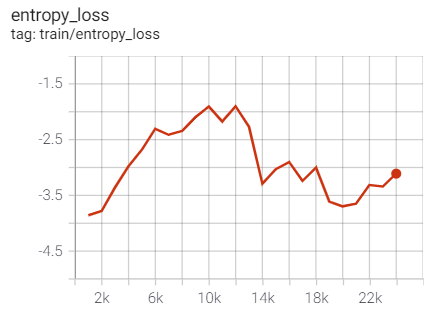
\includegraphics[scale=0.7]{pics/Tensorboard/A2C/entropy_loss.png}
  \caption{Entropieverlust}
  \label{fig:a2c:entropyloss}
\end{figure}


Das Modell, welches mit dem A2C Algorithmus trainiert, hat im Intervall von 0 bis 22.000 Schritten
konstant eine Lernrate von 0.0007. Diese wird von der ``Stable Baselines3''-Bibliothek als Standardwert
festgelegt.
Die folgende Funktion stellt die Lernrate der ``ScribbleFight'' Künstlichen Intelligenz dar.

\begin{figure}[H]
  \centering
  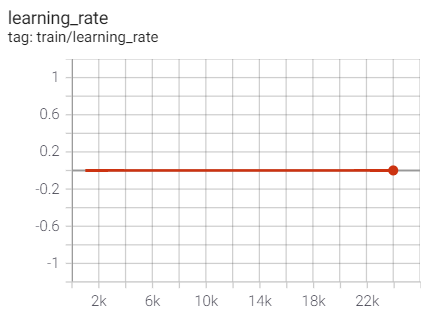
\includegraphics[scale=0.7]{pics/Tensorboard/A2C/learning_rate.png}
  \caption{Lernrate}
  \label{fig:a2c:learningrate}
\end{figure}

Auch im Falle des Wertverlusts ist kein klarer Trend erkennbar.
Dieser sollte steigen, so lange der Agent lernt. Wenn dieser Abfällt, oder gleichbleibend ist,
so spricht das dafür, dass die Künstliche Intelligenz ausgelernt hat und die Belohnung über die Zeit
nahezu gleich bleibend ist.

\begin{figure}[H]
  \centering
  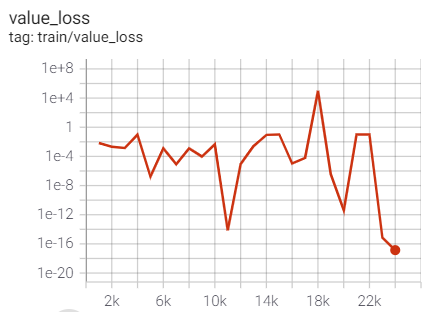
\includegraphics[scale=0.7]{pics/Tensorboard/A2C/value_loss_new.png}
  \caption{Wertverlust}
  \label{fig:a2c:valueLoss}
\end{figure}

Aus diesen Graphen ist es klar ersichtlich, dass der A2C Algorithmus für den Anwendungsfall nicht geeignet ist.


\subsubsection{PPO [H]}\label{maai:ppo:head}
Die Quelle zu folgendem Unterkapitel ist ein Blog auf der Website ``towardsdatascience.com'' mit dem Titel ``Proximal Policy Optimization Tutorial (Part 1/2: Actor-Critic Method)'' von ``Chintan Trivedi''. \cite{ppo:cite}

Der zweite Algorithmus, mit welchem die Künstliche Intelligenz trainiert wurde, heißt ``PPO''.
PPO ist eine Abkürzung und steht für ``Proximal Policy Optimization''. Dieses mathematische Modell
wurde von OpenAI im Jahr 2017 veröffentlicht. Es basiert darauf, dass eine kleine Menge an Erfahrung gesammelt wird, indem der Spieler mit seiner Umwelt interagiert.
Durch diese gesammelten Erfahrungen wird die Art und Weise zur Entscheidungsfindung angepasst; das heißt, dass die ``policy'' aktualisiert wird.
Nachdem die ``policy'' erneuert wurde, werden die gesammelten Erfahrungen verworfen und der Agent muss sich neu in der Umwelt orientieren, hat aber bereits mehr Basiswissen.
Dieser Ansatz wird auch ``on-policy learning'' genannt.

Der PPO-Algorithmus kümmert sich nun darum, dass die neue Vorgehensweise nicht zusehr von der alten abweicht.
Somit passiert weniger Varianz im Training der Künstlichen Intelligenz, wodurch einerseits ein schnelles Fortschreiten
beim Lernen verhindert wird, andererseits wird dabei sichergestellt, dass nichts ``falsches''
erlernt wird und somit nicht von einem gewünschtem Ziel abweicht.

% Quelle Diesmal wirklich zitat: https://towardsdatascience.com/proximal-policy-optimization-tutorial-part-1-actor-critic-method-d53f9afffbf6

Dass dieser Algorithmus besser funktioniert hat um die ScribbleFight KI zu trainieren wird durch folgenden
Graphen klar erkennbar.

Nach 900.000 Schritten passierte auch hier im Spiel ein Fehler, wordurch das Lernen abgebrochen ist.
Allerdings ließen sich dieses Ergebnisse im laufe der 25 Trainings, wobei die Hälfte mit dem PPO Algorithmus durchgeführt wurden,
jedes Mal replizieren.

Die Funktion des Entropieverlusts zeigt, dass die Aktionen, welche die KI durchführt, immer weniger zufällig
wurden.

\begin{figure}[H]
  \centering
  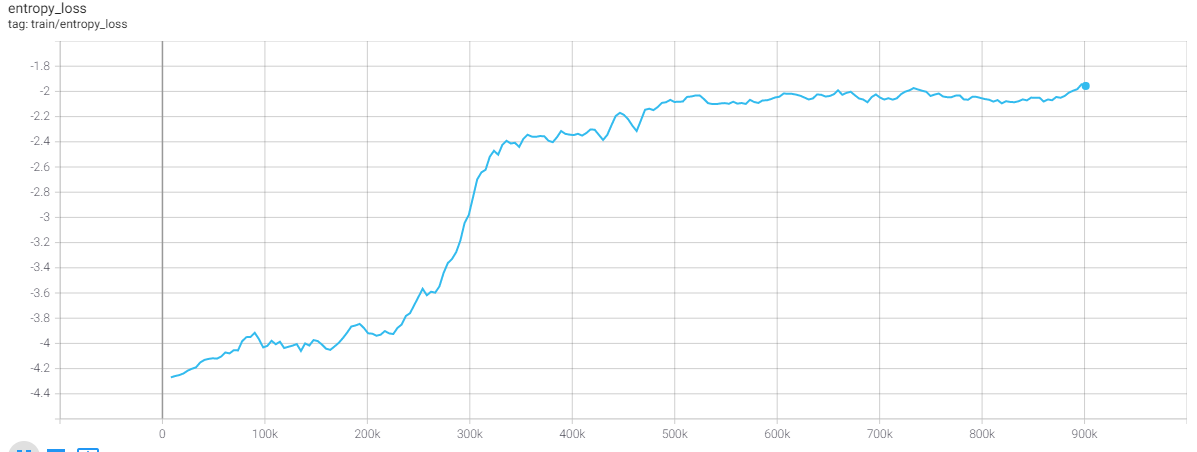
\includegraphics[scale=0.6]{pics/Tensorboard/PPO/entropy_loss.png}
  \caption{Entropieverlust}
  \label{fig:ppo:entropyloss}
\end{figure}

In der folgenden Grafik wird die Änderung der ``Policy-Loss''-Funktion beschrieben.
Diese zeigt, wie stark sich das Erlernte ändert und beschreibt somit den Prozess der Entscheidungsfindung.
Dadurch, dass die Funktion einen Verlust darstellt, sollte dieser in einem erfolgreichen Training fallen.
Die Werte sind während des Trainings stark geschwankt, was jedoch normal ist,
da durch den PPO Algorithmus die Policy Funktion in jeder Episode neu erlernt wird.
Die Aufgabe des mathematische Modells ist es, dass sich nur in Summe das Erlernte (``policy'') nicht zu stark in eine Richtung tendiert, wie am Anfang dieses Unterkapitels (\ref{maai:ppo:head}) erklärt ist.
Im Allgemeinen sollten die Werte der ``Policy-Loss''-Funktion kleiner als 1,0 sein.

\begin{figure}[H]
  \centering
  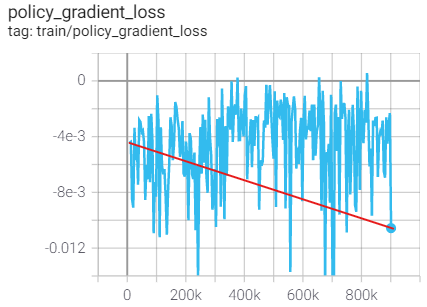
\includegraphics[scale=0.7]{pics/Tensorboard/PPO/policy_loss_new.png}
  \caption{Policy Graident Loss}
  \label{fig:ppo:pgl}
\end{figure}

Wie der ``Stable Baselines3''-Dokumentation %Site: \url{https://stable-baselines3.readthedocs.io/en/master/modules/ppo.html}
zu entnehmen ist, ist die Lernrate bei dem PPO Algorithmus eine Konstante.
Diese hat den Wert \(3*e^{-4}\).

\begin{figure}[H]
  \centering
  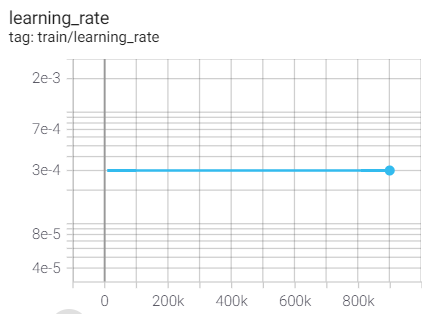
\includegraphics[scale=0.7]{pics/Tensorboard/PPO/learning_rate_new.png}
  \caption{Lernrate}
  \label{fig:ppo:learningrate}
\end{figure}

Obwohl das Modell, welches mit dem PPO-Algorithmus erlernt wurde,
bessere Ergebnisse erzielt hat, als jenes, welches mit dem A2C-Algorithmus trainiert wurde,
hat auch dieses viele Schwächen. So ist es nicht möglich, dass eine Vorhersage, welche
auf dem Erlernten basieren soll, einem menschlichen Spieler gleicht.


%Quelle: Tensorboard Dokumentation: https://www.tensorflow.org/tensorboard/get_started
% https://medium.com/aureliantactics/understanding-ppo-plots-in-tensorboard-cbc3199b9ba2

% TODO -
% Grafen beschreiben
% Quellen
% Ziel der KI beschreiben beim Difensio


% Siehe tolle Daten in Tab. \ref{tab:impl:data}.

% \begin{table}
%     \centering
%     \begin{tabular}{|lcc|}
%         \hline
%                   & \textbf{Regular Customers} & \textbf{Random Customers} \\ \hline
%         Age       & 20-40                      & \textgreater{}60          \\ \hline
%         Education & university                 & high school               \\ \hline
%     \end{tabular}
%     \caption{Ein paar tabellarische Daten}
%     \label{tab:impl:data}
% \end{table}

% \begin{figure}
%     \centering
%     
\includegraphics[scale=0.5]{pics/knuthi.jpg}
%     \caption{Don Knuth -- CS Allfather}
%     \label{fig:impl:knuth}
% \end{figure}

% Siehe und staune in Abb. \ref{fig:impl:knuth}.
% \lipsum[6-9]
% Dann betrachte den Code in Listing \ref{lst:impl:foo}.

% \begin{lstlisting}[language=Python,caption=Some code,label=lst:impl:foo]
% # Program to find the sum of all numbers stored in a list (the not-Pythonic-way)

% # List of numbers
% numbers = [6, 5, 3, 8, 4, 2, 5, 4, 11]

% # variable to store the sum
% sum = 0

% # iterate over the list
% for val in numbers:
%     sum = sum+val

% print("The sum is", sum)
% \end{lstlisting}